%%%%%%%%%%%%%%%%%%%%%%%%%%%%%%%%%%%%%%%%%%%%%%%
%%% Template for lab reports used at STIMA
%%%%%%%%%%%%%%%%%%%%%%%%%%%%%%%%%%%%%%%%%%%%%%%

%%%%%%%%%%%%%%%%%%%%%%%%%%%%%% Sets the document class for the document
% Openany is added to remove the book style of starting every new chapter on an odd page (not needed for reports)
\documentclass[12pt, english, openany]{book}
\usepackage[english]{babel}
\addto\captionsenglish{
  \renewcommand{\figurename}{Figure}
  \renewcommand{\tablename}{Table}
}
%%%%%%%%%%%%%%%%%%%%%%%%%%%%%% Loading packages that alter the style
\usepackage[]{graphicx}
\usepackage[]{color}
\usepackage{alltt}
\usepackage[T1]{fontenc}
\usepackage[utf8]{inputenc}
\setcounter{secnumdepth}{4}
\setcounter{tocdepth}{3}
\setlength{\parskip}{\smallskipamount}
\setlength{\parindent}{0pt}
\usepackage{titlesec}
\usepackage{listings}
\usepackage{amsmath}
\usepackage{xcolor}
% \usepackage{layouts}
\usepackage{eurosym}
\usepackage{siunitx}
%\usepackage[authoryear]{natbib}
\usepackage{placeins}
\usepackage{float}
\usepackage{csquotes}
\usepackage{tabularx} % add this in your preamble
\usepackage{subcaption}
\usepackage{tikz}
\definecolor{codegreen}{rgb}{0,0.6,0}
\definecolor{codegray}{rgb}{0.5,0.5,0.5}
\definecolor{codepurple}{rgb}{0.58,0,0.82}
\definecolor{backcolour}{rgb}{0.95,0.95,0.92}

\lstdefinestyle{mystyle}{
    backgroundcolor=\color{backcolour},   
    commentstyle=\color{codegreen},
    keywordstyle=\color{magenta},
    numberstyle=\tiny\color{codegray},
    stringstyle=\color{codepurple},
    basicstyle=\ttfamily\footnotesize,
    breakatwhitespace=false,         
    breaklines=true,                 
    captionpos=b,                    
    keepspaces=true,                 
    numbers=left,                    
    numbersep=5pt,                  
    showspaces=false,                
    showstringspaces=false,
    showtabs=false,                  
    tabsize=2
}

\lstset{style=mystyle}

% Package used for citations
% Adding both languages

\usepackage[
backend=biber,
style=numeric,
sorting=ynt
]{biblatex}
\addbibresource{bibliography.bib}


% Set page margins
\usepackage[top=100pt,bottom=100pt,left=68pt,right=66pt]{geometry}

% Package used for placeholder text
\usepackage{lipsum}

% Prevents LaTeX from filling out a page to the bottom
\raggedbottom



% All page numbers positioned at the bottom of the page
\usepackage{fancyhdr}
\fancyhf{} % clear all header and footers
\fancyfoot[C]{\thepage}
\renewcommand{\headrulewidth}{0pt} % remove the header rule
\pagestyle{fancy}

% Changes the style of chapter headings
\usepackage{titlesec}
\titleformat{\chapter}
   {\normalfont\LARGE\bfseries}{\thechapter.}{1em}{}
% Change distance between chapter header and text
\titlespacing{\chapter}{0pt}{0pt}{2\baselineskip}

% Adds table captions above the table per default
\usepackage{float}
\floatstyle{plaintop}
\restylefloat{table}

% Adds space between caption and table
\usepackage[tableposition=top]{caption}

% Adds hyperlinks to references and ToC
\usepackage{hyperref}
\usepackage{xurl}
\hypersetup{hidelinks,linkcolor = black} % Changes the link color to black and hides the hideous red border that usually is created

% If multiple images are to be added, a folder (path) with all the images can be added here 
\graphicspath{ {Figures/} }

%=== Farben definieren ========================================================
\definecolor{THRed}{RGB}{207,24,32}
\definecolor{THOrange}{RGB}{236,101,37}
\definecolor{THPurple}{RGB}{175,54,140}

% Separates the first part of the report/thesis in Roman numerals
\frontmatter

\usepackage[acronym]{glossaries}
\makeglossaries

\newacronym{mqtt}{MQTT}{Message Queuing Telemetry Transport}
\newacronym{nbiot}{NB-IoT}{Narrowband Internet of Things}
\newacronym{ltem}{LTE-M}{Long Term Evolution for Machines}
\newacronym{lwm2m}{LWM2M}{Lightweight Machine to Machine}
\newacronym{gnss}{GNSS}{Global Navigation Satellite System}
\newacronym{wifi}{WiFi}{Wireless Fidelity}
\newacronym{lte}{LTE}{Long Term Evolution}
\newacronym{lora}{LoRa}{Long Range}
\newacronym{lpwan}{LPWAN}{Low Power Wide Area Network}
\newacronym{tcp}{TCP}{Transmission Controll Protocoll}
\newacronym{udp}{UDP}{User Datagram Protocol}
\newacronym{coap}{CoAP}{Constrained Application Protocol}
\newacronym{gps}{GPS}{Global Positioning System}
\newacronym{gsm}{GSM}{Global System for Mobile Communications}
\newacronym{sigfox}{Sigfox}{Sigfox Network}
\newacronym{m2m}{M2M}{Machine to Machine}
\newacronym{iot}{IoT}{Internet of Things}
\newacronym{wlan}{WLAN}{Wireless Local Area Network}
\newacronym{soc}{SoC}{System on a Chip}
\newacronym{ble}{BLE}{Bluetooth Low Energy}
\newacronym{nfc}{NFC}{Near Field Communication}
\newacronym{rtos}{RTOS}{Real-Time Operating System}
\newacronym{sdk}{SDK}{Software Development Kit}
\newacronym{uart}{UART}{Universal Asynchronous Receiver-Transmitter}
\newacronym{supl}{SUPL}{Secure User Plane Location}
\newacronym{agnss}{AGNSS}{Assisted GNSS}
\newacronym{ttff}{TTFF}{Time to First Fix}
\newacronym{dtls}{DTLS}{Datagram Transport Layer Security}
\newacronym{tls}{TLS}{Transport Layer Security}
\newacronym{rsrp}{RSRP}{Reference Signal Received Power}
\newacronym{rsrq}{RSRQ}{Reference Signal Received Quality}
\newacronym{snr}{SNR}{Signal-to-Noise Ratio}
\newacronym{earfcn}{EARFCN}{E-UTRA Absolute Radio Frequency Channel Number}
\newacronym{apn}{APN}{Access Point Name}
\newacronym{tac}{TAC}{Tracking Area Code}
\newacronym{mcc}{MCC}{Mobile Country Code}
\newacronym{mnc}{MNC}{Mobile Network Code}
\newacronym{tau}{TAU}{Tracking Area Update}
\newacronym{ce}{CE}{Coverage Enhancement}
\newacronym{edrx}{eDRX}{Extended Discontinuous Reception}
\newacronym{vcom}{VCOM}{Virtual COM Port}
\newacronym{dl}{DL}{Downlink}
\newacronym{qpsk}{QPSK}{Quadrature Phase Shift Keying}
\newacronym{bpsk}{BPSK}{Binary Phase Shift Keying}
\newacronym{ofdma}{OFDMA}{Orthogonal Frequency Division Multiple Access}
\newacronym{scfdma}{SC-FDMA}{Single Carrier Frequency Division Multiple Access}
\newacronym{aes}{AES}{Advanced Encryption Standard}
\newacronym{mmtc}{mMTC}{Massive Machine-Type Communication}
\newacronym{psm}{PSM}{Power Saving Mode}
\newacronym{3gpp}{3GPP}{3rd Generation Partnership Project}
\newacronym{qam}{QAM}{Quadrature Amplitude Modulation}
\newacronym{ofdm}{OFDM}{Orthogonal Frequency Division Multiplexing}
\newacronym{papr}{PAPR}{Peak-to-Average Power Ratio}
\newacronym{fec}{FEC}{Forward Error Correction}
\newacronym{aka}{AKA}{Authentication and Key Agreement}
\newacronym{prb}{PRB}{Physical Resource Block}
\newacronym{harq}{HARQ}{Hybrid Automatic Repeat reQuest}
\newacronym{volte}{VoLTE}{Voice over LTE}
\newacronym{fota}{FOTA}{Firmware Over-The-Air}
\newacronym{snow}{SNOW}{SNOW 3G}
\newacronym{qos}{QoS}{Quality of Service}
\newacronym{psk}{PSK}{Pre-Shared Key}
\newacronym{rrc}{RRC}{Radio Resource Control}
\newacronym{ip}{IP}{Internet Protocol}
\newacronym{pcap}{PCAP}{Packet Capture}
\newacronym{nas}{NAS}{Non-Access Stratum}
\newacronym{api}{API}{Application Programming Interface}
\newacronym{kde}{KDE}{Kernel Density Estimation}
\newacronym{http}{HTTP}{Hypertext Transfer Protocol}
%%%%%%%%%%%%%%%%%%%%%%%%%%%%%% Starts the document
\begin{document}

%%% Selects the language to be used for the first couple of pages
\selectlanguage{english}

\begin{titlepage}
    %
    \sffamily% Umschalten auf serifenlose Schrift
    %
    \begin{center}
        
\begin{tikzpicture}
            \fill[THRed] (0, 0) rectangle (\textwidth/3, 3pt);
            \fill[THOrange] (\textwidth/3, 0) rectangle (2*\textwidth/3, 3pt);
            \fill[THPurple] (2*\textwidth/3, 0) rectangle (\textwidth, 3pt);
        \end{tikzpicture}
    \end{center}
    %
    \vfill
    %
    \begin{huge}
        Performance Evaluation of Data Collection for Outdoor Plant Experiments Based on NB-IoT and LTE-M\\[10mm]
    \end{huge}
    %
    Masterarbeit zur Erlangung des akademischen Grades\newline
    \emph{Master of Science}\newline
    im Studiengang Communication Systems and Networks\newline
    an der Fakultät für Informations-, Medien- und Elektrotechnik\newline
    der Technischen Hochschule Köln
    %
    \vfill
    %
    \begin{tabular}{@{}ll}
        vorgelegt von:     & Kai Lübeck                    \\
        Matrikel-Nr.:      & 11127675                      \\
        Adresse:           & Zülpicher Straße 231          \\
                           & 50937 Köln                    \\
                           & kai.luebeck@smail.th-koeln.de \\[5mm]
        eingereicht bei:   & Prof. Dr. Uwe Dettmar         \\
        Zweitgutachter*in: & Prof. Dr. Harald Elders-Boll
    \end{tabular}
    %
    \\[10mm]
    %
    Köln, 14.08.2025%
    %
    \rmfamily% Umschalten auf Standard-Schrift mit Serifen
    %
\end{titlepage}

% Adds a table of contents
\tableofcontents{}

\mainmatter

\chapter{Introduction} \label{chap:introduction}
\section{Motivation} \label{sec:motivation}

This project was motivated by the increasing need to collect reliable, high-resolution environmental data for plant experiments performed under outdoor conditions. Accurate monitoring of climate parameters is essential to understanding how plants respond to environmental changes, especially in the context of climate change and ecological research. This thesis is based on a collaboration between the Digital Communication Department at TH Köln and the Biology Department at Universität zu Köln. The collaboration focuses on improving methods for recreating real-world climate conditions in controlled environments.

The project's primary objective is to provide a framework for the collection of a wide range of climate parameters in outdoor settings. The goal of this project is to replicate these outdoor conditions within controlled indoor environments, such as climate chambers. This study will provide a scientific basis for analyzing the influence of climate change and various biological approaches on plant growth under realistic conditions.

In previous research, sensor systems for plant experiments were operated in closed indoor environments where robust internet infrastructure, such as \gls{wifi} or Ethernet, was available. However, as research continues to expand into outdoor applications, the lack of internet connectivity becomes a significant challenge for data acquisition and transmission. The development of technologies such as \gls{nbiot} and \gls{lte} has led to the promising solution of reliable and energy-efficient communication in remote and distributed sensor networks.

While prior studies have established a solid base of knowledge regarding the performance characteristics of \gls{lpwan} technology, a review of the existing literature reveals significant gaps in the evaluation of these technologies in outdoor settings. Prior studies have addressed specific aspects, including protocol efficiency, energy consumption analysis, and rural coverage planning. However, these studies lack a systemic analysis that integrates the performance of communication technology and the behavior of protocols under real-world outdoor conditions. Additionally, the concurrent evaluation of radio frequency parameters, protocol-specific metrics, and practical performance characteristics across multiple geographic locations has not been extensively explored in the existing research.

By testing \gls{nbiot} and \gls{lte} technologies in combination with \gls{mqtt} and \gls{lwm2m} protocols, this project aims to enable continuous collection of diverse sensor data, supporting more advanced analyses of plant-environment interactions. The research evaluates the performance characteristics of these protocol-technology combinations to determine optimal configurations for outdoor deployments. This work is expected to contribute to the scientific understanding of how climate variables influence plant growth while providing practical guidance for deploying reliable sensor networks in challenging outdoor environments using \gls{iot} communication protocols.

\section{Related Work} \label{sec:related_work}

This section reviews related studies investigating \gls{lpwan} technology and \gls{iot} protocol performance characteristics, providing context for the findings presented in this thesis.

\subsection{Protocol Performance in Cellular IoT Networks}

A study by Parmigiani and Dettmar evaluated \gls{lwm2m} and \gls{mqtt} performance over \gls{nbiot} and \gls{lte} networks, focusing on energy consumption and traffic efficiency \parencite{related_work_comparison}. The authors performed measurements using Raspberry Pi hardware with Quectel BG96 modems across European cellular networks in Slovakia and Italy. The study focuses on three scenarios: initial connection setup, single client-to-server messages, and steady-state updates under different security levels (no-security, \gls{psk}, certificates).

\textbf{Key Findings:} \gls{lwm2m} demonstrated superior efficiency during initial connection establishment, transferring 82\% and 61\% fewer bytes than \gls{mqtt} over \gls{lte} and \gls{nbiot} respectively. \gls{mqtt} outperformed \gls{lwm2m} for large payload transmissions, consuming 20\% less energy for single message transfers. For small payloads below MTU threshold, \gls{lwm2m} showed 44\% lower energy consumption. During steady-state operations, the effect of the chosen protocol became irrelevant due to the effects of the \gls{rrc} inactivity timer.

\subsection{Energy Consumption Analysis}

A energy consumption study by Vomhoff et al. investigated power characteristics of \gls{nbiot} and \gls{ltem} using Arduino MKR NB 1500 platforms with high-precision Tinkerforge measurement equipment \parencite{related_work_energy_consumption}. The research created a cost-efficient testbed achieving 1mW energy monitoring resolution and evaluated network attachment procedures and data transmission with \gls{http} and \gls{mqtt} protocols.

\textbf{Key Findings:} Network attachment consumed significantly more energy for \gls{nbiot} compared to \gls{ltem}, while \gls{nbiot} demonstrated superior idle efficiency. Devices maintaining long-term connections benefited from \gls{nbiot}, whereas applications requiring frequent reconnections achieved lower consumption with \gls{ltem}. \gls{mqtt} had higher connection overhead than \gls{http} but provided more efficient data transmission for smaller payloads.

\subsection{Coverage and Capacity Analysis}

A rural deployment study by Lauridsen et al. investigated \gls{lte} and \gls{nbiot} performance across 800 km² of Danish territory using commercially deployed base station configurations and calibrated propagation models \parencite{related_work_coverage_capacity}. The simulation-based approach incorporated 71 sectors with realistic antenna patterns, transmit power configurations, and digital elevation maps, calibrated against drive test measurements.

\textbf{Key Findings:} \gls{lte} achieved 99.9\% outdoor coverage while \gls{nbiot} provided superior deep indoor performance with 164 dB Maximum Coupling Loss versus \gls{lte}'s 156 dB MCL. Under challenging indoor conditions, \gls{lte} supported 80,000 devices per sector versus 5,000 for \gls{nbiot} with full security protocols. \gls{nbiot} devices consumed 2-6 times more power than \gls{lte} primarily due to \gls{rrc} delay overheads, though battery life estimates exceeded 5 years.

\subsection{Similarities and Differences}

All three studies share the same objective of empirically evaluating \gls{nbiot} and \gls{lte} performance characteristics, using real-world measurement approaches rather than theoretical analysis. The studies consistently identify energy efficiency trade-offs between the technologies, with \gls{nbiot} demonstrating coverage advantages at the cost of higher connection overhead.

Key differences include hardware platforms (Raspberry Pi, Arduino, simulation), geographic focus (European multi-location, single testbed, rural Denmark), and evaluation scope (protocol comparison, energy analysis, coverage planning). The measurement approaches vary from direct hardware measurements to calibrated simulations, providing diverse perspectives on technology performance.

\subsection{Research Gap and Contribution}

The reviewed literature establishes foundational understanding of LPWAN performance trade-offs but reveals gaps in outdoor deployment evaluation. While existing studies focus on specific aspects (protocol efficiency, energy consumption, rural coverage), none provide integrated analysis of radio frequency parameters, protocol behavior, and practical performance metrics under real-world outdoor conditions. The current thesis addresses this gap by performing systematic outdoor measurements that simultaneously analyze cellular technology performance and protocol interaction dependencies, providing practical guidance for outdoor environmental monitoring deployments.


\section{Objectives} \label{sec:objectives}

The present thesis is an evaluation of the performance of two cellular technologies, \gls{nbiot} and \gls{lte}, in the context of outdoor plant monitoring. The study focuses on the suitability of these technologies when used with two popular IoT communication protocols:  \gls{mqtt} and \gls{lwm2m}. The objective of this study is to determine efficient, reliable, and context-appropriate combinations of protocol and technology for transmitting data in constrained outdoor environments.

This study addresses critical gaps identified in the existing literature regarding the comparative performance of \gls{mqtt} and \gls{lwm2m} under real-world conditions, especially over narrowband cellular communication links. Although prior studies have shown that \gls{lwm2m} offers enhanced efficiency during the establishment of connections and that \gls{mqtt} performs more effectively for transmitting large payloads, these studies have been restricted to specific deployment scenarios or have concentrated on individual performance aspects, such as energy consumption or the analysis of rural coverage. The performance boundaries under which \gls{mqtt} could outperform CoAP-based \gls{lwm2m} despite its theoretical inefficiencies, namely, overhead and connection-oriented nature, have not been systematically evaluated across outdoor deployment conditions. Such conditions include radio frequency parameters, protocol behavior, and practical performance metrics.

Furthermore, the efficacy of protocol implementation is dependent on the characteristics of the underlying cellular technology. However, no study has yet provided an integrated analysis of all four protocol-technology combinations under identical environmental conditions. Those combinations are \gls{nbiot}/\gls{mqtt}, \gls{nbiot}/\gls{lwm2m}, \gls{lte}/\gls{mqtt} and \gls{lte}/\gls{lwm2m}. A review of the existing literature reveals a consistent identification of trade-offs between technologies in terms of energy efficiency. However, an evaluation of the dependencies between protocols and technologies is lacking. Such an evaluation is critical for informed deployment decisions in outdoor monitoring scenarios.

A key component of the project was the development of a robust, automated measurement setup which includes hardware as well as software, that addresses several limitations observed in previous studies. Those limitations are the fact that most of the exisiting research if focusing on a single metric or performance indicator, while this study aims to include a huge variety of metrics. The system's design was based on the principle of reproducibility, which aimed to ensure consistent testing across different hardware configurations, communication protocols, and network environments. A primary emphasis was placed on the aggregation and structuring of collected data to support cross-parameter analysis. The resulting dataset includes a wide range of parameters, ranging from signal quality and connection metrics for example snr, rsrp, rsrq to protocol-specific metrics such as timing or latency.
The collected data should also be a resource for future research, enabling further interpretation and analysis that goes beyond the scope of this thesis. Upon completion of the project, the dataset will be open-sourced to support open scientific research.\footnote{\url{https://github.com/MrPink1996/Performance-Evaluation-of-Data-Collection-for-Outdoor-Plant-Experiments-Based-on-NB-IoT-and-LTE-M}}

To achieve the research objective and address the identified research gaps, the following measurable outcomes are targeted:

\begin{itemize}
    \item Perform a quantitative evaluation of key network performance indicators, including data throughput, end-to-end latency, connection setup time, stability, and coverage, under changing environmental and locational conditions across multiple geographic measurement points.
    \item Perform simultaneous comparison of \gls{mqtt} and \gls{lwm2m} protocol behavior on both \gls{nbiot} and \gls{ltem} networks to establish protocol-technology interaction dependencies.
    \item Identify deployment-specific trade-offs, such as protocol overhead, energy efficiency, and communication reliability, in outdoor experimental setups through integrated analysis of radio frequency parameters and protocol-specific metrics.
    \item Determine optimal protocol-technology combinations for specific use cases within agricultural and environmental \gls{iot} applications through empirical research that addresses gaps in existing literature.
\end{itemize}

\section{Structure of the Thesis} \label{sec:structure}
The following chapters are organized to provide a detailed overview of the thesis.\\
\hyperref[chap:theoretical_background]{Chapter~\ref*{chap:theoretical_background}} introduces the theoretical background on \gls{nbiot}, \gls{ltem}, \gls{mqtt}, and \gls{lwm2m}.\\
\hyperref[chap:implementation]{Chapter~\ref*{chap:implementation}} describes the implementation, including hardware and software components, the measurement setup, and the challenges faced during the project.\\
\hyperref[chap:measurements]{Chapter~\ref*{chap:measurements}} presents the measurement results and describes the data analysis methods.\\
\hyperref[chap:discussion]{Chapter~\ref*{chap:discussion}} discusses the interpretation of results, compares \gls{nbiot} and \gls{ltem} as well as \gls{mqtt} and \gls{lwm2m}, and addresses the limitations of the study.\\
\hyperref[chap:conclusion]{Chapter~\ref*{chap:conclusion}} summarizes the findings and offers recommendations for future work.\\
Finally, \hyperref[chap:outlook]{Chapter~\ref*{chap:outlook}} provides an outlook on potential future developments in data collection for outdoor plant experiments.

\chapter{Theoretical Background} \label{chap:theoretical_background}
\section{NB-IoT} \label{sec:nbiot}


\gls{nbiot}, classified as LTE Category NB1 (Cat-NB1), is a cellular communication technology standardized by the \gls{3gpp} as part of the Release~13 specifications \parencite{NBIOT_SYSTEM}. It is specifically designed to support massive Machine-Type Communication (\gls{mmtc}) applications within the \gls{iot} ecosystem. \gls{nbiot} addresses critical requirements such as extended coverage, low power consumption, massive device connectivity, and optimized network resource utilization, making it suitable for scenarios such as smart metering, environmental monitoring, and asset tracking.

\subsection{Frequency Usage and Deployment Modes}

\gls{nbiot} operates in licensed spectrum within existing cellular frequency bands and can be deployed in three distinct modes \parencite{NBIOT_SYSTEM}:

\begin{itemize}
    \item \textbf{In-band deployment:} Utilizes resource blocks within an existing \gls{lte} carrier's bandwidth, allowing \gls{nbiot} to coexist with \gls{lte} users.
    \item \textbf{Guard-band deployment:} Fills up unused resource blocks in the guard bands of \gls{lte} carriers to avoid interference and improve spectral efficiency.
    \item \textbf{Standalone deployment:} Operates independently within reused \gls{gsm} spectrum (e.g., a 200\,kHz \gls{gsm} channel), making use of legacy infrastructure and providing deployment flexibility in rural or remote areas.
\end{itemize}

\gls{nbiot} uses a narrow carrier bandwidth of \SI{180}{kHz}, equivalent to a single \gls{lte} \gls{prb}. This design choice ensures cost-efficiency in transceiver hardware and improves indoor penetration by concentrating energy over a narrowband.

\subsection{Physical Layer and Modulation Schemes}

The physical layer of \gls{nbiot} is based on \gls{lte} technology, with simplifications for cost and coverage optimization \parencite{NBIOT_PHYSICAL_LAYER}. It supports different modulation and access schemes for uplink and downlink:

\begin{itemize}
    \item \textbf{Downlink:} \gls{nbiot} employs \gls{ofdma} with a subcarrier spacing of \SI{15}{kHz}, matching \gls{lte}. \gls{ofdma} divides the spectrum into orthogonal subcarriers, allowing multiple users to transmit simultaneously without mutual interference. The modulation scheme used in the downlink is typically \gls{qpsk}, ensuring a balance between spectral efficiency and robustness.

    \item \textbf{Uplink:} Two modes are supported: single-tone and multi-tone transmissions. Uplink access uses \gls{scfdma}, which, unlike \gls{ofdma}, transmits data in a single carrier with a lower \gls{papr}, ideal for energy-constrained \gls{iot} devices. Depending on configuration:
          \begin{itemize}
              \item \textbf{Single-tone:} Uses one subcarrier (\SI{3.75}{kHz} or \SI{15}{kHz}) with \gls{bpsk} or \gls{qpsk} modulation.
              \item \textbf{Multi-tone:} Uses up to 12 subcarriers, each spaced at \SI{15}{kHz}, occupying the full \SI{180}{kHz} bandwidth, with \gls{qpsk} modulation.
          \end{itemize}
\end{itemize}

These physical layer characteristics are designed to enhance coverage and minimize energy consumption, even in conditions with poor signal strength \parencite{NBIOT_PHYSICAL_LAYER}.

\subsection{Channel Coding and Error Correction}

\gls{nbiot} uses robust error correction and coding techniques derived from \gls{lte}, which have been adapted for low data rates and enhanced coverage \parencite{NBIOT_PHYSICAL_LAYER}.

\begin{itemize}
    \item \textbf{Downlink:} Employs Turbo codes, which are powerful \gls{fec} schemes known for near-Shannon-limit performance.
    \item \textbf{Uplink:} Uses convolutional codes, which are less complex than Turbo codes, making them suitable for energy-efficient uplink transmissions.
\end{itemize}

Furthermore, repetition coding is a fundamental technique in the field of \gls{nbiot}, where messages are transmitted multiple times to improve reliability in low \gls{snr} environments. This repetition has been shown to improve coverage by up to \SI{20}{dB} in comparison with standard \gls{lte} \parencite{NBIOT_SYSTEM}.

\subsection{Bandwidth, Throughput, and Latency}

Due to its narrow bandwidth of \SI{180}{kHz}, \gls{nbiot} offers modest data throughput but is sufficient for most \gls{iot} use cases \parencite{NBIOT_SYSTEM}:

\begin{itemize}
    \item \textbf{Downlink:} Peak data rate up to \SI{127}{kbps}.
    \item \textbf{Uplink:} Peak rate up to \SI{159}{kbps} using 12-tone multi-tone transmission. In single-tone mode, uplink rates are significantly lower, typically around \SI{66}{kbps}.
\end{itemize}

Latency in \gls{nbiot} is optimized for small, infrequent data transmissions. Depending on network conditions, repetition, and power-saving configurations, latency ranges from \SI{1.6}{s} to over \SI{10}{s}.

\subsection{Security Aspects}

The security architecture of \gls{nbiot} is derived from \gls{lte}, thereby ensuring robust protection for user and signaling data \parencite{NBIOT_WIKI}.

\begin{itemize}
    \item \textbf{Mutual authentication:} Between the device and the network using standardized \gls{3gpp} \gls{aka} protocols.
    \item \textbf{Encryption:} Based on secure algorithms like \gls{snow} and \gls{aes}, protecting data confidentiality.
    \item \textbf{Integrity protection:} Ensures signaling messages are not altered in transmissions.
    \item \textbf{Dynamic key management:} Cryptographic keys are generated and refreshed periodically during secure sessions.
\end{itemize}

The mechanisms, when considered together, ensure secure end-to-end communication suitable for critical \gls{iot} applications.

\subsection{Power Consumption and Energy Efficiency}

The design of \gls{nbiot} is focused on energy-constrained IOT devices \parencite{NBIOT_POWER}. The primary mechanisms that contribute to extending battery life beyond 10 years are as follows:

\begin{itemize}
    \item \textbf{\gls{psm}:} The device enters a deep sleep state while remaining registered to the network. No downlink reception occurs, reducing power draw to microampere levels.
    \item \textbf{\gls{edrx}:} The device periodically wakes up to check for messages. Idle cycles are extended up to several minutes, dramatically lowering average power consumption.
\end{itemize}

These features are critical for devices deployed in remote areas where frequent maintenance is impractical \parencite{NBIOT_POWER}.

\subsection{Network Parameter Evaluation}

\gls{nbiot} performance can be analyzed using standard communication metrics \parencite{NBIOT_SYSTEM}:

\begin{itemize}
    \item \textbf{Spectral Efficiency:} Although \gls{nbiot} uses narrow bandwidth, its modulation and coding schemes ensure spectral efficiency around 0.2-1.4\,bit/s/Hz depending on link conditions.
    \item \textbf{Coverage Enhancement:} Link budget improvements of up to \SI{20}{dB} allow connectivity in basements, rural, and underground locations.
    \item \textbf{Massive Connectivity:} More than 50,000 devices per cell should be supported.
    \item \textbf{Reliability:} Enhanced by \gls{harq}, convolutional coding, and repetition techniques.
    \item \textbf{Latency-Throughput Tradeoff:} Although not suitable for real-time applications, it demonstrates optimal performance in energy-efficient, delay-tolerant communication.
\end{itemize}

\subsection{Summary}

It is widely acknowledged that \gls{nbiot} plays a fundamental role in ensuring the effective operation of large-scale \gls{iot} networks \parencite{NBIOT_SYSTEM}. The device's narrowband operation, simplified physical layer, and optimized power consumption contribute to secure, long-range, and low-cost connectivity. Despite its constrained throughput and real-time capabilities, the device demonstrates notable strengths in scenarios that require extended battery life, extensive coverage, and secure low-bandwidth data exchange.

\section{LTE-M} \label{sec:ltem}

\gls{ltem}, specifically \gls{lte} Category M1 (Cat-M1), is a \gls{lpwan} technology that has been standardized by the \gls{3gpp} in Release~13 \parencite{LTE_SYSTEM}. It is designed to support \gls{iot} applications requiring higher data rates, reduced latency, and mobility support compared to \gls{nbiot}. Positioned between legacy \gls{lte} and \gls{nbiot}, \gls{ltem} offers a balanced trade-off between throughput and power efficiency for use cases such as wearables, asset tracking, and \gls{volte}-enabled sensors.

\subsection{Frequency Usage and Deployment Modes}

\gls{ltem} operates within licensed \gls{lte} spectrum and supports \parencite{LTE_SYSTEM}:

\begin{itemize}
    \item \textbf{In-band deployment:} \gls{lte} is integrated into the same \gls{lte} carrier bandwidth as traditional \gls{lte} traffic, taking advantage of dynamic resource allocation across the shared spectrum.
\end{itemize}

Unlike \gls{nbiot}, \gls{ltem} does not support guard-band or standalone deployment modes. It uses a bandwidth of \SI{1.4}{MHz}, equivalent to six \gls{lte} \gls{prb}, enabling higher data rates and improved spectral efficiency.

\subsection{Physical Layer and Modulation Schemes}

The physical layer of \gls{ltem} is largely derived from \gls{lte}, with specific optimizations for the purpose of reducing device complexity and enhancing power efficiency \parencite{LTE_SYSTEM}.

\begin{itemize}
    \item \textbf{Downlink:} Uses Orthogonal Frequency Division Multiplexing (\gls{ofdm}) with a subcarrier spacing of \SI{15}{kHz}, identical to \gls{lte}. Supported modulation schemes include \gls{qpsk} and 16-\gls{qam}, enabling a good balance between spectral efficiency and robustness.

    \item \textbf{Uplink:} Uses \gls{scfdma} with \SI{15}{kHz} subcarrier spacing. It supports both \gls{qpsk} and 16-\gls{qam}, allowing scalable uplink data rates based on channel conditions and power requirements.
\end{itemize}

In contrast to the \gls{nbiot}, the \gls{ltem} offers support for mobility and higher-order modulation, making it well-suited for devices that require real-time data exchange and roaming capabilities.

\subsection{Channel Coding and Error Correction}

\gls{ltem} reuses \gls{lte}'s robust error correction schemes \parencite{LTE_SYSTEM}:

\begin{itemize}
    \item \textbf{Downlink:} Turbo coding provides powerful \gls{fec}, ensuring data integrity in poor channel conditions.
    \item \textbf{Uplink:} Control channels often use convolutional codes for lower computational complexity, while data channels continue to use Turbo codes.
\end{itemize}

\gls{harq} is also implemented, combining \gls{fec} with retransmission for improved reliability.

\subsection{Bandwidth, Throughput, and Latency}

With its \SI{1.4}{MHz} bandwidth, \gls{ltem} offers significantly higher throughput and lower latency than \gls{nbiot} \parencite{LTE_SYSTEM}:

\begin{itemize}
    \item \textbf{Downlink:} Peak throughput of up to \SI{1}{Mbps}, sufficient for voice, messaging, and \gls{fota} updates.
    \item \textbf{Uplink:} Data rates up to \SI{375}{kbps}, depending on modulation and resource allocation.
    \item \textbf{Latency:} Typically between \SI{10}{ms} and \SI{15}{ms}, which supports delay-sensitive applications such as alarms or voice.
\end{itemize}

The selected performance metrics are well-suited for use cases which require moderate, bidirectional data flows.

\subsection{Mobility and Handover Support}

\gls{ltem} has been developed to support continuous cell reselection and handover, including idle and connected mode mobility, making it suitable for mobile \gls{iot} applications such as vehicle tracking, logistics, and mobile health monitoring \parencite{LTE_SYSTEM}. Additionally, it supports \gls{volte}, allowing for real-time voice communication over cellular \gls{iot} devices.

\subsection{Security Aspects}

\gls{ltem} maintains \gls{lte}'s full security architecture \parencite{LTEM_WIKI}:

\begin{itemize}
    \item \textbf{Mutual authentication:} Ensures secure identity verification via the standardized \gls{3gpp} \gls{aka} protocol.
    \item \textbf{Encryption and integrity:} Both user and signaling data are protected with \gls{aes} and \gls{snow} algorithms.
    \item \textbf{Key management:} Session keys are dynamically generated and periodically refreshed to ensure confidentiality.
\end{itemize}

This robust security framework supports trusted communication in critical and sensitive \gls{iot} applications.

\subsection{Power Consumption and Energy Efficiency}

While offering higher link throughput, the system still focuses on energy-efficient operation through the following mechanisms \parencite{LTEM_POWER}:

\begin{itemize}
    \item \textbf{\gls{psm}:} Allows the device to enter a deep-sleep state while retaining network context, minimizing energy consumption between transmissions.
    \item \textbf{\gls{edrx}:} Reduces power usage by decreasing the frequency of downlink listening periods, adjustable based on application needs.
\end{itemize}

These features support battery lifetimes of up to 10 years, depending on the data transmission profile \parencite{LTEM_POWER}.

\subsection{Network Parameter Evaluation}

Key performance indicators for \gls{ltem} include \parencite{LTE_SYSTEM}:

\begin{itemize}
    \item \textbf{Spectral Efficiency:} Higher than \gls{nbiot} due to wider bandwidth and support for 16-\gls{qam}, typically around 1-3\,bit/s/Hz depending on link conditions.
    \item \textbf{Coverage Enhancement:} Provides up to \SI{15}{dB} gain over legacy \gls{lte}, enabling reliable connections in deep indoor and remote environments.
    \item \textbf{Latency-Throughput Tradeoff:} Offers improved latency and throughput, but with slightly higher energy cost compared to \gls{nbiot}.
\end{itemize}

\subsection{Summary}

The \gls{ltem} standard is a technological advancement that increases \gls{lte}'s capabilities to the Internet of Things (IoT) domain, thereby enabling applications that require mobility, moderate data rates, and low latency \parencite{LTE_SYSTEM}. The device's compatibility with existing infrastructure originates from its support for in-band and guard-band deployment in combination with standard \gls{lte} modulation and coding schemes. While not as energy-optimized as \gls{nbiot}, its wider range of features makes it an ideal solution for a wide range of smart connected devices.

\section{MQTT} \label{sec:mqtt}

The \gls{mqtt} protocol is a lightweight, publish-subscribe network protocol designed for efficient message transport between devices in distributed systems \parencite{MQTT_WIKI}. It is optimized for resource-constrained environments and communication over low-bandwidth, high-latency, or unreliable networks, making it suitable, especially for \gls{iot} applications and \gls{m2m} communication \parencite{naik2017choice}.

\subsection{Architectural Model}

\gls{mqtt} is based on a broker-client architecture, which differs fundamentally from traditional client-server models \parencite{naik2017choice}. Its core components include:

\begin{itemize}
    \item \textbf{Broker:} A central entity that receives all messages, filters them according to their topics, and forwards them to subscribed clients.
    \item \textbf{Clients:} Devices or applications that publish data to topics or subscribe to topics to receive data.
\end{itemize}

Communication occurs over \textit{topics}, which are hierarchical UTF-8 strings. Clients publish messages to a topic, and subscribers receive those messages asynchronously. This decoupling made scalable and flexible communication patterns possible.

\subsection{Transport Layer and Connection Establishment}

\gls{mqtt} uses \gls{tcp} as its transport layer protocol \parencite{naik2017choice}. Key aspects include:

\begin{itemize}
    \item \textbf{Three-way handshake:} Required to establish a \gls{tcp} connection before \gls{mqtt} communication.
    \item \textbf{Connection state maintenance:} \gls{tcp} maintains permanent connections, allowing continuous sessions essential for \gls{iot} use cases.
\end{itemize}

Frequent connection disruptions (e.g., in wireless networks) require repeated handshakes, increasing latency and resource consumption.

\subsection{Messaging and Quality of Service}

\gls{mqtt} communication involves several control packets:

\begin{itemize}
    \item \textbf{CONNECT, PUBLISH, SUBSCRIBE, DISCONNECT}
\end{itemize}

It supports three QoS levels \parencite{MQTT_WIKI}:

\begin{enumerate}
    \item \textbf{QoS 0 (At most once):} Unreliable but low overhead.
    \item \textbf{QoS 1 (At least once):} Reliable with possible duplication.
    \item \textbf{QoS 2 (Exactly once):} Most reliable, highest overhead.
\end{enumerate}

These allow flexibility between reliability, latency, and resource use.

\subsection{Performance Considerations in Connection Stability}

Unstable connections lead to increased overhead from repeated handshakes and session reinitialization, reducing throughput and increasing energy use. Optimizing connection persistence is critical in such scenarios \parencite{naik2017choice}.

\subsection{Visualization of Connection Establishment}

Figures \ref{fig:MQTT_CONN} and \ref{fig:MQTT_QOS} illustrating client-broker interaction including \gls{tcp} handshake, \gls{mqtt} session setup, and \gls{qos}-based message flow.

\begin{figure}[htbp]
    \centering
    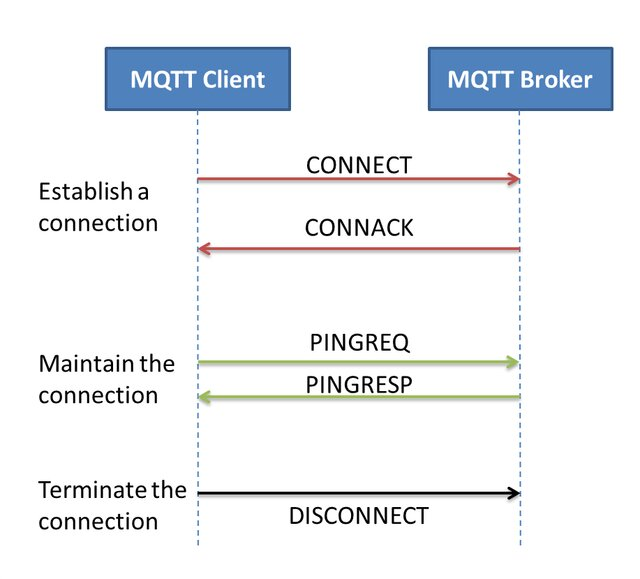
\includegraphics[width=1\textwidth]{MQTT_CONN.jpg}
    \caption{
        \textbf{MQTT Connection Establishment} \\
        The picture shows the typical phases of the client-broker connection in \gls{mqtt}. \parencite{MQTT}
    }
    \label{fig:MQTT_CONN}
\end{figure}

\begin{figure}[htbp]
    \centering
    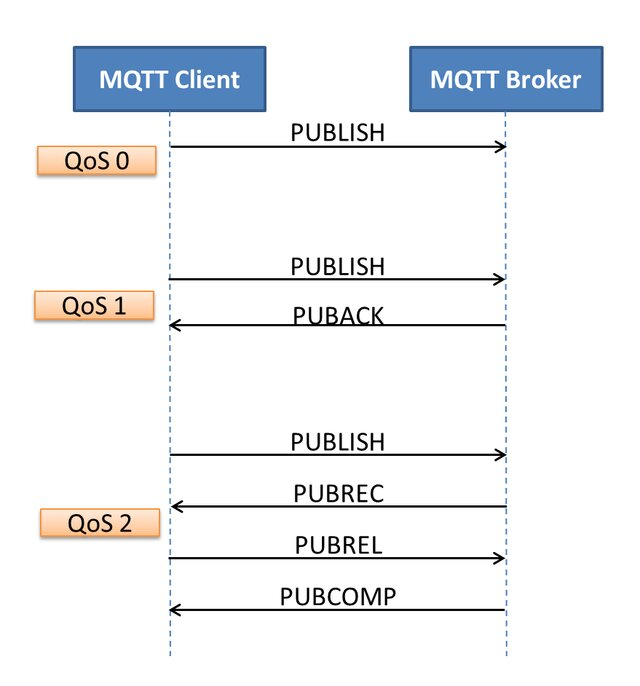
\includegraphics[width=1\textwidth]{MQTT_QOS.jpg}
    \caption{
        \textbf{MQTT Messaging} \\
        The picture shows the behavior when transmitting messages with different \gls{qos} parameters. \parencite{MQTT}
    }
    \label{fig:MQTT_QOS}
\end{figure}

\subsection{Security Features and Mechanisms}

While \gls{mqtt} is lightweight and lacks built-in security, typical implementations rely on \parencite{MQTT_WIKI}:

\begin{itemize}
    \item \textbf{\gls{tls} encryption}
    \item \textbf{Client authentication (username/password, certificates)}
    \item \textbf{Broker-side access control}
    \item \textbf{Message integrity/replay protection via \gls{tls}}
\end{itemize}

Security depends on proper configuration of these additional mechanisms.

\subsection{Summary}

\gls{mqtt} enables lightweight, publish-subscribe messaging, which is well-suited for \gls{iot} applications \parencite{naik2017choice}. It is not equipped with built-in security features, but it can be secured through the use of \gls{tls} and broker-based controls. This approach provides scalable and secure communication within constrained environments.

%-----------------------------------------------------

\section{LWM2M} \label{sec:lwm2m}

The \gls{lwm2m} protocol is a standardized protocol developed by the Open Mobile Alliance for the efficient management of resource-constrained \gls{iot} devices \parencite{oma_lwm2m_2017}. This system supports remote configuration, telemetry, and lifecycle management \parencite{LWM2M_WIKI}.

\subsection{Architectural Model}

LwM2M follows a \textit{client-server architecture}, focusing on remote device management \parencite{oma_lwm2m_2017}. Core elements include:

\begin{itemize}
    \item \textbf{LwM2M Client:} Usually an embedded device or sensor that exposes resources.
    \item \textbf{LwM2M Server:} Manages clients by reading/writing values and issuing commands.
\end{itemize}

The model is based on hierarchical \textit{objects}, \textit{instances}, and \textit{resources}, enabling standardized device interaction.

\subsection{Transport Layer and Connection Establishment}

\gls{lwm2m} uses the \gls{coap} over \gls{udp} \parencite{oma_lwm2m_2017}:

\begin{itemize}
    \item \textbf{\gls{udp} transport:} Reduces overhead and supports faster communication compared to \gls{tcp}.
    \item \textbf{Reliability mechanisms:} \gls{coap} provides confirmable messages, retransmissions, and deduplication to ensure reliable communication.
\end{itemize}

This enables efficient, low-latency communication suitable for battery-powered devices.

\subsection{Messaging and QOS}

\gls{lwm2m} messaging uses \gls{coap}'s RESTful methods (GET, POST, PUT, DELETE) and includes \parencite{oma_lwm2m_2017}:

\begin{itemize}
    \item \textbf{Read/write operations}
    \item \textbf{Execute commands}
    \item \textbf{Bootstrap procedures}
    \item \textbf{Observation of resources}
\end{itemize}

Quality and reliability are handled via \gls{coap}'s confirmable/non-confirmable messages. While not using \gls{qos} levels like \gls{mqtt}, it achieves similar guarantees through message acknowledgments and retransmissions.

\subsection{Performance Considerations in Connection Stability}

Operating over \gls{udp} allows for low overhead but requires robust retransmission logic. The lightweight reliability mechanisms of \gls{coap} serve to reduce the impact of interrupted connectivity, thereby enabling \gls{lwm2m} to operate over unreliable links while preserving energy efficiency \parencite{oma_lwm2m_2017}.

\subsection{Visualization of Connection Phases}

Analogous to \gls{mqtt}, \gls{lwm2m} involves a multi-step process:

\begin{itemize}
    \item \gls{udp} transmission initiation
    \item \gls{dtls} handshake (if security enabled)
    \item \gls{coap}-based messaging and observation
    \item Optional bootstrap and resource management
\end{itemize}

\subsection{Security Features and Mechanisms}

\gls{lwm2m} provides strong built-in security \parencite{oma_lwm2m_2017}:

\begin{itemize}
    \item \textbf{\gls{dtls} encryption} over \gls{udp}
    \item \textbf{Authentication:} Pre-shared keys, raw public keys, or certificates
    \item \textbf{Fine-grained access control} on resources
    \item \textbf{Replay protection} via \gls{dtls} features
\end{itemize}

These security features are fundamental to the protocol and are essential for protecting managed devices from unauthorized access or control.

\subsection{Summary}

\gls{lwm2m} is a comprehensive protocol for managing constrained IoT devices \parencite{LWM2M_WIKI}. The \gls{coap} messaging over \gls{udp}, hierarchical resource modeling, and robust security via \gls{dtls} enable scalable and secure device management in distributed \gls{iot} environments \parencite{oma_lwm2m_2017}.

\section{Comparison of NB-IoT and LTE-M} \label{sec:comparison_nbiot_ltem}


\begin{table}[htbp]
    \centering
    \caption{Comparison of Key Features between LTE-M and NB-IoT}
    \label{tab:ltem_vs_nbiot}
    \begin{tabularx}{\textwidth}{|l|X|X|}
        \hline
        \textbf{Feature}         & \textbf{LTE-M}                         & \textbf{NB-IoT }                                            \\ \hline
        3GPP Category            & Cat-M1                                 & Cat-NB1                                                     \\ \hline
        Carrier Bandwidth        & \SI{1.4}{MHz} (6 PRBs)                 & \SI{180}{kHz} (1 PRB)                                       \\ \hline
        Deployment Modes         & In-band only                           & In-band, Guard-band, Standalone (re-farmed GSM)             \\ \hline
        Modulation Schemes       & QPSK, 16-QAM (DL/UL)                   & BPSK, QPSK (mostly)                                         \\ \hline
        Peak Downlink Throughput & Up to \SI{1}{Mbps}                     & Up to \SI{127}{kbps}                                        \\ \hline
        Peak Uplink Throughput   & Up to \SI{375}{kbps}                   & Up to \SI{159}{kbps} (12-tone), \SI{66}{kbps} (single-tone) \\ \hline
        Latency                  & Typically 10–15 ms                     & Typically \SI{1.6}{s} to \SI{10}{s}                         \\ \hline
        Mobility Support         & Full LTE mobility and handover support & Limited mobility, no handovers                              \\ \hline
        Coverage Enhancement     & Approx. 15 dB over LTE                 & Up to 20 dB over LTE                                        \\ \hline
        Power Saving Features    & PSM, eDRX                              & PSM, eDRX                                                   \\ \hline
        Security                 & LTE-grade (AKA, encryption, integrity) & LTE-grade (AKA, encryption, integrity)                      \\ \hline
        Typical Applications     & Asset tracking, wearables, VoLTE       & Smart metering, environmental monitoring                    \\ \hline
        Device Complexity        & Moderate                               & Very low                                                    \\ \hline
    \end{tabularx}
\end{table}

\FloatBarrier



\section{Comparison of MQTT and LwM2M} \label{sec:comparison_mqtt_lwm2m}
\begin{table}[htbp]
    \centering
    \caption{Comparison of Key Features between LwM2M and MQTT}
    \label{tab:lwm2m_vs_mqtt}
    \begin{tabularx}{\textwidth}{|l|X|X|}
        \hline
        \textbf{Feature}                    & \textbf{LwM2M}                                                & \textbf{MQTT}                                                    \\ \hline
        Protocol Type                       & Device management and telemetry                               & Lightweight messaging protocol (telemetry)                       \\ \hline
        Transport Layer                     & UDP (via CoAP)                                                & TCP                                                              \\ \hline
        Communication Model                 & Client-Server (RESTful)                                       & Broker-based Publish/Subscribe                                   \\ \hline
        Data Model                          & Hierarchical: Object / Instance / Resource                    & Flat, topic-based string hierarchy                               \\ \hline
        Message Encoding                    & Compact binary (Efficient XML Interchange or CBOR)            & Text or binary payloads, no strict structure                     \\ \hline
        Reliability Mechanism               & CoAP confirmable messages, retransmission, deduplication      & QoS levels 0 (at most once), 1 (at least once), 2 (exactly once) \\ \hline
        Security                            & Built-in DTLS (PSK, RPK, X.509); integrated replay protection & Relies on TLS and broker-side access control                     \\ \hline
        Device Management                   & Full: provisioning, firmware update, resource monitoring      & Not natively supported; possible via custom payloads             \\ \hline
        Suitability for Constrained Devices & High (optimized for low-power, low-memory devices)            & Moderate (requires persistent TCP connection)                    \\ \hline
        Connection Overhead                 & Low (UDP, stateless, no keep-alive)                           & Moderate (TCP handshake and keep-alive required)                 \\ \hline
        Session Persistence                 & Stateless by design; can reconnect without session context    & Stateful; relies on persistent TCP session                       \\ \hline
        Use Cases                           & Device lifecycle management, telemetry, firmware updates      & Sensor telemetry, alerts, asynchronous event notifications       \\ \hline
        Standardization Body                & OMA SpecWorks                                                 & OASIS                                                            \\ \hline
    \end{tabularx}
\end{table}

\FloatBarrier

\chapter{Implementation} \label{chap:implementation}
\section{Hardware Overview} \label{sec:hardware_overview}



The implementation and testing of this project was carried out using the nRF9160 Development Kit from Nordic Semiconductor. The core of the kit is the nrf9160 \gls{soc}, which integrates an energy-efficient Arm Cortex-M33 application processor and a dedicated cellular modem supporting both \gls{nbiot} (Cat-NB1) and \gls{ltem} (Cat-M1) technologies. The nRF9160 System in Package (SiP) is specifically designed to support Long-Term Evolution (LTE) Cat-M1 and Cat-NB1, providing full LPWAN connectivity capabilities for IoT applications.

The nRF9160 \gls{soc} integrates multiple peripheral interfaces for sensor integration and includes an integrated \gls{gps} module, which enables precise geolocation functionality. This feature is advantageous for mobile or spatially distributed \gls{iot} deployments. Furthermore, the development board includes a distinct nRF52840 \gls{soc} that provides support for \gls{ble} and \gls{nfc}, though these wireless interfaces are not used in this project.

The nRF9160 Development Kit is well-suited for prototyping and evaluating \gls{iot} applications in constrained environments due to its low-power operation, wide-area connectivity, and flexible peripheral support. This performance-focused study identified the nRF9160 Development Kit as an optimal selection. As illustrated in Figure \ref{fig:NRF9160DK}, a general overview of the hardware is provided.

For the purpose of this study, two identical nRF9160 Development Kits were used in parallel: one configured to run an \gls{lwm2m}-based implementation, and the other dedicated to \gls{mqtt} communication combined with \gls{gnss}-based location tracking. This enabled the simultaneous evaluation of both protocol stacks under comparable field conditions.


\begin{figure}[htbp]
    \centering
    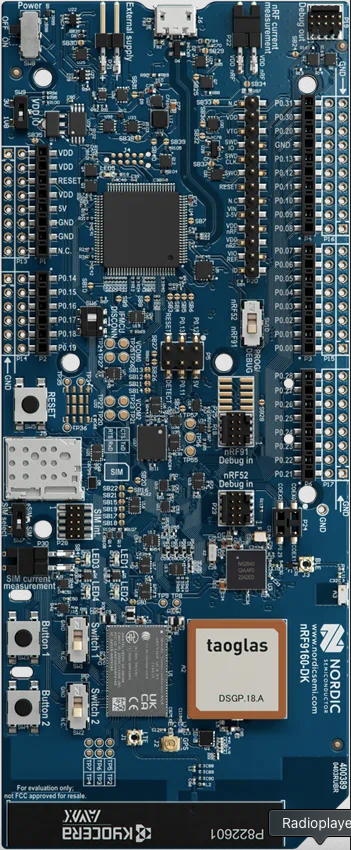
\includegraphics[scale=0.6]{nrf9160DK.png}
    \caption{
        \textbf{nRF9160 Development Kit} \\
        Nordic Semiconductor nRF9160 Development Kit showing the main circuit board with integrated cellular and GPS antennas, USB connector, and development interface pins.
    }
    \vspace{0.5em}
    \textcolor{gray}{\footnotesize \textit{Source: \url{https://www.nordicsemi.com/Products/Development-hardware/nRF9160-DK}}}
    \label{fig:NRF9160DK}
\end{figure}




\section{Software Overview} \label{sec:software_overview}

The software environment used in this project was designed to align with the hardware capabilities of the NRF9160 and to support robust, low-power communication protocols suitable for \gls{iot} deployments. This chapter presents an overview of the operating system, development tools, protocol stacks, backend infrastructure, and data analysis frameworks used during the implementation and testing phases.

\subsection{Operating System and SDK}

The firmware for both experimental devices was based on the Zephyr \gls{rtos} version 2.9.1. Zephyr is a lightweight, scalable, and modular \gls{rtos} designed for resource-constrained embedded systems. It offers support for Nordic Semiconductor hardware platforms. The primary motivation for its selection was its close integration with Nordic's development environment, along with its wide community and industrial support.

The project was developed using the nRF Connect \gls{sdk} (v2.9.1), which is the official \gls{sdk} from Nordic Semiconductor built on top of Zephyr. The \gls{sdk} offers a range of essential components, including device drivers, board support packages, protocol libraries, and example applications. The basis for this project was two Zephyr sample applications:

\begin{itemize}
    \item \texttt{lwm2m\_client}: used for the \gls{lwm2m} implementation and extended to support sensor simulation and performance logging.
    \item \texttt{mqtt\_simple}: used as a foundation for \gls{mqtt} testing, including custom \gls{gnss} integration and performance metrics collection.
\end{itemize}

\subsection{Development Environment}

The development of the entire software was implemented through the use of Visual Studio Code on a macOS platform. Nordic's toolchain and dependencies were managed using the west meta-tool. The firmware was installed on the nRF9160 boards via USB, and debugging was managed using \gls{uart} logging mechanisms.

\subsection{GNSS and AGNSS Integration}

For \gls{gnss} positioning, the firmware included \gls{agnss} functionality, which used \gls{supl} data from Google's \gls{supl} server. This strategy leads to a reduction in time, which was found to be significant in low-power and cold-start scenarios, where it was critical to minimize the \gls{ttff}.

\subsection{Communication Infrastructure}

In this project, two separate \gls{iot} communication protocols were evaluated: The first is the \gls{mqtt} protocol, and the second is the \gls{lwm2m} protocol. The implementation of these systems was based on independent server infrastructures.

\begin{itemize}
    \item \textbf{LwM2M Server:} The public \textit{Eclipse Leshan} demo server was used to manage and observe the \gls{lwm2m} client device. Communication occurred over \gls{dtls} with \gls{psk} authentication for encrypted transport.
    \item \textbf{MQTT Broker:} A private \textit{Mosquitto} \gls{mqtt} broker (version 2.0.11) was hosted on a local Raspberry Pi running in a home server setup. Secure communication was ensured using \gls{tls} with certificate-based authentication.
\end{itemize}

\subsection{Data Storage and Backend Processing}

Collected measurement data from both devices was stored in a PostgreSQL 15.10 database running on the same Raspberry Pi server as the \gls{mqtt} broker. A custom Python (v3.12.9) application was developed to:
\begin{itemize}
    \item Receive and parse messages from \gls{mqtt}.
    \item Write telemetry and metadata to the PostgreSQL database.
    \item Aggregate, analyze, and visualize performance metrics across both technologies and protocols.
\end{itemize}

Python libraries such as \texttt{psycopg2}, \texttt{pandas}, and \texttt{matplotlib} were employed for data processing, visualization, and statistical comparison. The data aggregation from both boards is further detailed in Section~\ref{sec:measurement_setup}.

\subsection{Multi-Board Setup}

Two separate nRF9160 Development Kits were used in parallel for the duration of the experiments. One device was dedicated to running the \gls{lwm2m} client, while the other simultaneously executed the \gls{mqtt} client application with \gls{gnss} tracking enabled. This dual-board configuration enabled synchronized and unbiased performance comparisons between the two protocol stacks under identical environmental and network conditions.

\section{Measurement setup} \label{sec:measurement_setup}

To ensure extensive performance evaluation, both nRF9160 Development Kits were configured with \gls{uart}-based logging capabilities. It has been determined that each board is equipped with a \gls{vcom} interface via USB, which provides three virtual serial ports. These include:

\begin{itemize}
    \item \textbf{VCOM Port 0} was used for general application logging, including output from the main firmware (e.g., network statistics, \gls{gps} data, timing metrics).
    \item \textbf{VCOM Port 2} (the third port) was reserved for capturing raw modem traces, which consist of binary diagnostic data generated directly by the cellular modem.
\end{itemize}

The identification of each board was facilitated by its unique device ID, a feature that allowed the Python data acquisition scripts to dynamically assign the correct serial interfaces to the respective \gls{mqtt} and \gls{lwm2m} clients. Both development kits were connected to a macOS host system via a powered USB hub.


\subsection{Firmware Workflow and Test Procedure}

The firmware executed on each development kit was designed to emulate realistic application-layer traffic patterns while allowing precise control over network selection and data flow. The experiment was structured into three phases per device, executed in a controlled sequence to ensure comparable performance conditions.

\paragraph{MQTT and GNSS Board}

The board assigned to the \gls{mqtt} workload followed a three-step operation pattern:

\begin{enumerate}
    \item \textbf{GNSS Initialization and Fix Acquisition:}
          Upon boot, the firmware initiates a connection to the cellular network, choosing between \gls{ltem} and \gls{nbiot} based on the internal Zephyr network selection logic, which evaluates available signal quality and connection readiness. Once connected, the board requests \gls{supl} assistance data over the active link to accelerate \gls{ttff} for the onboard \gls{gnss} module. The system then awaits a valid position fix. After that, the cellular connection is gracefully released.

    \item \textbf{MQTT Uplink via LTE-M:}
          The firmware reconnects to the cellular network, this time explicitly selecting the \gls{ltem} access technology. A fixed-size payload of 128 bytes is transmitted to a designated \gls{mqtt} broker using \gls{mqtt} version 3.1.1 with \gls{qos} level 0, which provides "at most once" delivery semantics. After transmission, the device disconnects from the network.

    \item \textbf{MQTT Uplink via NB-IoT:}
          The same procedure is repeated, but the device connects via \gls{nbiot} instead of \gls{ltem}. The same 128-byte payload is transmitted to the \gls{mqtt} broker using \gls{mqtt} version 3.1.1 with \gls{qos} 0. Following this, the firmware stops execution.
\end{enumerate}

This operational structure allowed for a direct comparison between \gls{ltem} and \gls{nbiot} uplink performance within the same environmental and hardware constraints, with \gls{gnss} serving as an additional performance parameter for initial fix acquisition under assisted conditions.

\paragraph{LwM2M Board}

The second board, used for \gls{lwm2m} evaluation, executed a similar sequence, but with a distinct communication stack and use case:

\begin{enumerate}
    \item \textbf{LwM2M Session over LTE-M:}
          The board establishes a cellular connection explicitly over \gls{ltem} and connects to a remote \gls{lwm2m} server. Upon successful registration, a local Python script running on the host system triggers a series of sample data reads via the \gls{lwm2m} interface. Simultaneously, the script captures logs and modem traces. After a delay of 20 seconds to allow interaction and background communication, the board disconnects from the \gls{ltem} network.

    \item \textbf{LwM2M Session over NB-IoT:}
          The board reattaches to the network, this time using the \gls{nbiot} radio access technology, and repeats the process: establishing a connection with the \gls{lwm2m} server, enabling the Python script to perform the same read operations. After data collection, the firmware disconnects and stops execution.
\end{enumerate}

By executing \gls{lwm2m} communication on both \gls{ltem} and \gls{nbiot} sequentially within the same firmware cycle, the setup provides a direct comparison of end-to-end latency, registration time, and protocol responsiveness across both radio technologies.

\subsection{Data Collection and Logging Framework}

A custom Python 3.12 script was developed using the pyserial library to continuously monitor and log data from all active \gls{uart} ports. The script simultaneously managed the two boards, extracting and timestamping performance metrics in real-time. The following parameters were logged:

\begin{itemize}
    \item \textbf{Network Parameters:}
          \begin{itemize}
              \item Network Mode (\gls{ltem} or \gls{nbiot})
              \item \gls{apn}
              \item \gls{tac}
              \item \gls{mcc} and \gls{mnc}
              \item Frequency Band and \gls{earfcn}
              \item Cell ID and Physical Cell ID
              \item Transmission Power, Repetition Counts (Tx/Rx), \gls{ce} level
              \item \gls{edrx} cycle
              \item Signal quality metrics: \gls{rsrp}, \gls{rsrq}, \gls{snr}, and \gls{dl} Pathloss
              \item \gls{tau} configuration and triggers
              \item Link quality estimate and Energy Estimate
          \end{itemize}

    \item \textbf{Connection Performance:}
          \begin{itemize}
              \item Time required to attach to the cellular network
              \item Time to establish a connection to the respective application-layer protocol (\gls{mqtt} or \gls{lwm2m})
              \item Basic uplink throughput metrics based on fixed-size \gls{udp} payloads
          \end{itemize}

    \item \textbf{Geolocation Data:}
          \begin{itemize}
              \item \gls{gps} coordinates retrieved from the \gls{mqtt}-enabled device via \gls{gnss} logging
          \end{itemize}
\end{itemize}

The parsing of this information was executed in real-time, and the resultant data was stored in a PostgreSQL 15.10 database that was located on the same Raspberry Pi server that was being used to operate the \gls{mqtt} broker. This enabled efficient querying, post-processing, and data correlation across multiple experiments and geographic locations.

\subsection{Modem Trace Analysis}

To support the high-level logging, low-level modem traces were collected in parallel from both boards. The modem trace data, which was captured via the \gls{vcom} trace port, was converted from its binary format into industry-standard .pcapng files using Nordic's nrfutil trace tool. These files allow for detailed packet-level inspection using Wireshark or programmatic analysis with the pyshark library.

Despite not being stored directly in the database due to their size and complexity, the .pcapng traces were archived and subsequently analyzed during the evaluation phase. This analysis was used to validate observed performance anomalies, retransmissions, and protocol behavior under different network conditions.

\subsection{Parallelized Testing}

During the experimental phase, both boards were operated in parallel. The \gls{lwm2m} client was executed on one device, while the second board simultaneously ran the \gls{mqtt} client with \gls{gnss} functionality. This parallelized approach ensured synchronized measurement conditions across both protocols and cellular technologies, thus minimizing temporal and environmental biases in the collected performance data.

\section{Challenges} \label{sec:challenges}

A number of technical and methodological challenges were encountered during the implementation and evaluation phases of this project, particularly in the areas of low-level data acquisition, protocol trace analysis, and automation of the measurement framework.

\subsection{Modem Trace Extraction and Analysis}

A notable challenge was the extraction and interpretation of modem trace data from the nRF9160 development boards. These traces, which consist of raw binary logs generated by the cellular modem, are essential for undertaking a detailed analysis of protocol behavior and network-layer interactions. However, the process of converting these binary files into a human-readable format proved to be non-trivial.

At the beginning, the documentation provided minimal guidance on the interpretation and decoding of modem trace files. After a detailed investigation, the \texttt{nrfutil trace} utility was identified as the appropriate tool for converting the binary logs into the industry-standard .pcapng format, which can be analyzed using Wireshark. After conversion, the interpretation of the trace content required a significant investment of time and effort due to two factors. Firstly, there was a lack of detailed documentation, which made it difficult to understand the data. Secondly, the number of packets per session was extremely high, which further complicated the analysis. The process of identifying relevant protocol messages (e.g., attach requests, handovers, retransmissions) within extensive and frequently noisy traces proved to be a manual effort of significant duration.
\subsection{Throughput Measurement Implementation}

Another technical challenge encountered was the implementation of a basic throughput measurement over the raw cellular link using \gls{udp}. Link throughput was measured using a UDP-based uplink speed test, where the device transmitted a 512-byte payload to a remote server. The server calculated immediate throughput by measuring the time difference between packet arrivals using precise kernel timestamps, accounting for all protocol headers (\gls{udp}, \gls{ip}, Ethernet). This metric represents the effective uplink data rate achievable under current radio frequency conditions.

The measurement approach employed a two-packet timing method: the client first sends a 1-byte trigger message followed immediately by the 512-byte data payload. The server captures nanosecond-precision timestamps for both packets and calculates throughput based on the second packet's total size (554 bytes including headers) divided by the inter-packet arrival time. In consideration of the constrained nature of the embedded environment and the limitations of the underlying network stack, close attention was required to ensure optimal performance metrics, including packet sizing, buffering, and timing accuracy.

This approach was implemented to ensure the reliability and reproducibility of the experimental results, providing a standardized measurement of immediate uplink throughput rather than theoretical link capacity. This was crucial during the testing phase under \gls{nbiot} conditions, where constrained bandwidth and high latency can readily introduce distortions in performance metrics, requiring precise timing measurements to accurately capture the effective data transmission capabilities.
\subsection{Measurement Framework Stability and Automation}

The establishment of a reliable and reproducible measurement configuration was found to be a time-consuming process. The objective of the study was to collect a wide range of performance metrics (e.g., signal strength, connection time, \gls{gps} location, throughput) across two parallel devices in a consistent and synchronized manner. The successful integration of these components, which included UART logging, modem trace conversion, \gls{gps} data capture, protocol-level timing, and database storage, was essential for the achievement of this objective.

Ensuring that the setup was sufficiently robust to operate autonomously for extended periods and under varying network conditions presented additional challenges. To ensure the accuracy and reliability of the data, multiple iterations were necessary to refine the Python-based logging and aggregation scripts, address serial port conflicts, and manage edge cases such as dropped connections or incomplete logs.

\chapter{Measurements} \label{chap:measurements}


The measurements produced a total of 312 datasets, including 156 datasets for the MQTT protocol and 156 datasets for the \gls{lwm2m} protocol. Each dataset contains 27 parameters, which were obtained directly from the nRF9160 development board. Furthermore, for each dataset, there is a corresponding pcapng file that stores modem information, resulting in a total of 312 pcapng modem traces. The measurements were conducted in 156 different locations within the Cologne area, as illustrated in Figure \ref{fig:measurement_points_map}.


% Figure: Measurement Points Map
\begin{figure}[htbp]
    \centering
    \includegraphics[width=0.9\textwidth]{MeasurementPoints.png}
    \caption{\textbf{Data Collection Locations} \\ The figure shows the distribution of the 156 measurement locations. Each marker represents a single conducted measurement.}
    \label{fig:measurement_points_map}
\end{figure}


\subsection*{Protocol-Specific Metrics from PCAP Analysis}

The following parameters were extracted from modem trace files converted to \gls{pcap} format and analyzed using pyshark. These metrics provide insights into low-level protocol behavior and network interaction patterns.

\begin{itemize}
    \item \textbf{Retransmissions} \hfill [count] \\
          Number of packet retransmissions observed during a communication session. The calculation method varies by protocol:

          \textbf{MQTT (TCP-based):} Retransmissions are detected by analyzing \gls{tcp} sequence numbers and acknowledgment patterns on port 8883. The analysis tracks outgoing packets with their sequence numbers and matches them with incoming acknowledgments. Retransmissions are identified when duplicate sequence numbers appear or when acknowledgments arrive out of order, indicating that packets were lost and required retransmission by the \gls{tcp} protocol stack.

          \textbf{LWM2M (UDP-based):} Since \gls{udp} is connectionless, retransmissions must be detected at the application layer through \gls{coap} request-response pairing. The analysis automatically detects \gls{lwm2m} communication ports (typically 5683, 5684, 5000, 8000) and tracks outgoing \gls{coap} requests. Retransmissions are counted when requests are sent without corresponding responses within reasonable timeout periods, indicating that the \gls{coap} confirmable message mechanism triggered retransmission due to lost or delayed packets.

    \item \textbf{Latency} \hfill [s] \\
          End-to-end latency measured differently for each protocol based on their underlying transport mechanisms:

          \textbf{MQTT Latency Calculation:} Measured by analyzing \gls{tcp} acknowledgment timing for packets on port 8883. The analysis tracks the time difference between when a \gls{tcp} segment is transmitted and when its corresponding acknowledgment is received. This provides insight into the round-trip time for \gls{mqtt} communication, filtered to include only realistic latency values between 0-5 seconds to exclude measurement artifacts and packet reordering effects.

          \textbf{LWM2M Latency Calculation:} Based on \gls{coap} request-response timing patterns. The analysis measures the time between outgoing \gls{coap} requests to \gls{lwm2m} servers and their corresponding responses. This application-layer latency measurement captures the end-to-end responsiveness of the \gls{lwm2m} protocol, with filtering applied to include only response times between 0-10 seconds to account for the potentially higher latency characteristics of constrained networks.

    \item \textbf{Security Handshake Time} \hfill [s] \\
          Time required to complete the security establishment phase for encrypted connections:

          \textbf{MQTT TLS Handshake:} Detected through analysis of \gls{tcp} payload sizes and patterns on port 8883. The analysis identifies \gls{tls} handshake phases by examining payload characteristics: small initial packets (~20-50 bytes) indicate Client Hello messages, large subsequent packets (>100 bytes) suggest Server Hello and certificate exchange, followed by key exchange and finished messages. The handshake duration is measured from the first \gls{tls} packet to the completion of the certificate exchange phase.

          \textbf{TLS Handshake Phases Detected:}
          \begin{enumerate}
              \item Client Hello (small payload ~20-50 bytes)
              \item Server Hello + Certificate (large payload >100 bytes)
              \item Key Exchange (medium payload)
              \item Finished Messages (small payload)
          \end{enumerate}

          \textbf{LWM2M DTLS Handshake:} Employs similar heuristic approaches applied to \gls{udp} traffic on \gls{lwm2m} ports, though \gls{dtls} detection presents additional challenges due to \gls{udp}'s connectionless nature. The analysis identifies \gls{dtls} handshake patterns by examining packet sizes and timing patterns characteristic of \gls{dtls} certificate exchange and key establishment procedures.

    \item \textbf{RRC State Changes} \hfill [count] \\
          Number of Radio Resource Control state transitions observed during a communication session. These are extracted from AT command responses embedded in the \gls{pcap} trace data. The analysis monitors for specific AT command indicators that signal RRC state transitions, particularly focusing on connection establishment and release events.

          \textbf{CSCON Status Codes \parencite{CSCON_STATUS_CODES}:}
          \begin{itemize}
              \item \texttt{+CSCON: 0} = \gls{rrc} Idle (radio connection released)
              \item \texttt{+CSCON: 1} = \gls{rrc} Connected (radio connection active)
          \end{itemize}

          Frequent \gls{rrc} state changes impact energy consumption and connection stability, especially relevant for battery-powered outdoor sensors.

    \item \textbf{Network Registration Changes} \hfill [count] \\
          Number of network registration state changes occurring during a communication session. Extracted by monitoring \gls{nas} (Non-Access Stratum) signaling messages captured in the modem trace data. The analysis tracks changes in network registration status by parsing AT command responses that indicate registration state transitions.

          \textbf{CEREG Status Codes \parencite{CREG_STATUS_CODES}:}
          \begin{itemize}
              \item \texttt{+CEREG: 0} = Not registered, not searching
              \item \texttt{+CEREG: 1} = Registered, home network
              \item \texttt{+CEREG: 2} = Not registered, searching
              \item \texttt{+CEREG: 3} = Registration denied
              \item \texttt{+CEREG: 4} = Unknown
              \item \texttt{+CEREG: 5} = Registered, roaming
          \end{itemize}

          High values suggest network instability or mobility-related issues that could affect outdoor sensor reliability and indicate potential connectivity problems during deployment.
\end{itemize}

\subsection*{Data Processing and Filtering}

The \gls{pcap} analysis implements several filtering mechanisms to ensure data quality:

\textbf{Latency Filtering:}
\begin{itemize}
    \item \gls{mqtt} latencies outside 0-5000ms range are excluded
    \item \gls{lwm2m} response times outside 0-10000ms range are excluded
    \item Filters eliminate unrealistic values caused by packet reordering
\end{itemize}

\textbf{Signal Quality Filtering:}
\begin{itemize}
    \item AT command values of 255 are treated as invalid measurements
    \item Empty or malformed AT responses are ignored
    \item Only complete measurement sequences are included in analysis
\end{itemize}

\textbf{Session Boundary Detection:}
\begin{itemize}
    \item Sessions are automatically split based on \texttt{AT\%XSYSTEMMODE} commands
    \item Protocol-specific port detection enables accurate traffic classification
    \item Incomplete sessions without clear boundaries may result in partial analysis
\end{itemize}

These parameters form the basis for evaluating cellular link reliability, protocol responsiveness, and deployment-specific performance characteristics across communication technologies and protocol layers. The combination of modem \gls{api} data, custom timing measurements, and \gls{pcap} trace analysis provides comprehensive visibility into both radio-level and protocol-level performance characteristics essential for outdoor deployment planning.


\section{Data Processing and Analysis Methodology} \label{sec:data_processing_and_analysis_methodology}

The collected measurement data was processed and analyzed using Python 3.12. A custom analysis pipeline was developed to extract metrics, generate visualizations, and enable comparative evaluations across different communication technologies and application protocols.

\subsection*{Software Stack and Libraries}

The following Python libraries were used during the measurement collection and analysis:

\begin{itemize}
    \item \texttt{pyserial}: for serial communication with nRF9160 development kits and AT command interface
    \item \texttt{paho-mqtt}: for \gls{mqtt} client implementation and protocol testing
    \item \texttt{pyshark}: for \gls{pcap} file analysis and network packet inspection
    \item \texttt{scapy}: for packet capture and network traffic analysis
    \item \texttt{pandas}, \texttt{numpy}: for numerical operations, statistical analysis, and structured data processing
    \item \texttt{scipy.stats}: for statistical testing including Mann-Whitney U tests and Kruskal-Wallis analysis
    \item \texttt{matplotlib.pyplot}, \texttt{seaborn}: for static 2D visualizations, including boxplots and statistical plots
    \item \texttt{json}, \texttt{os}: for handling configuration files, data storage, and directory traversal
    \item \texttt{requests}: for HTTP-based communication and server interactions
    \item \texttt{threading}, \texttt{queue}: for concurrent measurement execution and data collection
\end{itemize}

All measurement logs were stored in structured formats (JSON and PCAPNG), parsed using specialized libraries, and analyzed in Jupyter Notebooks and standalone Python scripts for full performance evaluation.
\subsection*{Visualization and Statistical Methods}

The following visual and statistical techniques were used to present and explore the measurement data:

\begin{itemize}
    \item \textbf{Confidence Interval Plots:} These plots display the mean value of a metric along with its confidence interval, providing insight into the statistical reliability and variability of the measurements. For a given confidence level $\alpha$ (typically 95\%), the confidence interval for the population mean $\mu$ is calculated as \parencite{CONFIDENCE_INTERVAL}:

          \[
              CI = \bar{x} \pm t_{\alpha/2, n-1} \cdot \frac{s}{\sqrt{n}}
          \]

          where:
          \begin{itemize}
              \item $\bar{x}$ is the sample mean
              \item $t_{\alpha/2, n-1}$ is the critical value from the t-distribution with $n-1$ degrees of freedom
              \item $s$ is the sample standard deviation
              \item $n$ is the sample size
          \end{itemize}

          The confidence interval represents the range within which the true population mean is likely to fall with the specified confidence level. These plots are valuable for comparing performance metrics between different protocol-technology combinations while accounting for measurement uncertainty.

          \textbf{Statistical significance testing in confidence interval plots:} To determine whether observed differences between groups are statistically significant, hypothesis testing is performed beside the confidence interval visualization. The choice of statistical test depends on the number of groups being compared:

          \textbf{Mann-Whitney U Test:} A non-parametric statistical test used for comparing two independent groups (e.g., \gls{nbiot} vs. \gls{ltem}) \parencite{MANN_WHITNEY_U_TEST}. This test is suitable when data does not meet the assumptions of parametric tests (normality, equal variances). The Mann-Whitney U test checks whether one group tends to have larger values than the other by ranking all observations and comparing rank sums between groups.

          \textbf{Kruskal-Wallis Test:} A non-parametric statistical test used when comparing multiple independent groups (e.g., all four protocol-technology combinations: \gls{mqtt}+\gls{nbiot}, \gls{mqtt}+\gls{ltem}, \gls{lwm2m}+\gls{nbiot}, \gls{lwm2m}+\gls{ltem}) \parencite{KRUSKAL_WALLIS_TEST}. This test extends the Mann-Whitney U test to more than two groups and checks whether the median values differ significantly across groups. The test statistic H is calculated as:

          \[
              H = \frac{12}{N(N+1)} \sum_{i=1}^{k} \frac{R_i^2}{n_i} - 3(N+1)
          \]

          where:
          \begin{itemize}
              \item $k$ is the number of groups being compared
              \item $N$ is the total number of observations across all groups
              \item $n_i$ is the number of observations in group $i$
              \item $R_i$ is the sum of ranks for group $i$
          \end{itemize}

          \textbf{p-value interpretation:} The p-value represents the probability of observing the measured difference (or a more extreme difference) between groups, assuming the null hypothesis (no difference between groups) is true \parencite{P_INTERPRETATION}. Conventional interpretation levels are:
          \begin{itemize}
              \item $p < 0.001$: Highly significant (***) - very strong evidence against the null hypothesis
              \item $p < 0.01$: Significant (**) - strong evidence against the null hypothesis
              \item $p < 0.05$: Significant (*) - moderate evidence against the null hypothesis
              \item $p \geq 0.05$: Not significant (ns) - insufficient evidence to reject the null hypothesis
          \end{itemize}

          These statistical tests ensure objective determination of whether observed performance differences between groups are statistically meaningful rather than due to random variation. The Mann-Whitney U test is used for two-group comparisons (technology comparisons), while the Kruskal-Wallis test is used for multi-group comparisons (protocol-technology combination analysis).

    \item \textbf{Kernel Density Estimation (KDE):} A non-parametric statistical method used to estimate the probability density function of a continuous random variable from a finite dataset \parencite{KDE_FUNCTION}. Unlike histograms, \gls{kde} provides a smooth, continuous estimate of the underlying distribution. The \gls{kde} estimator is defined as:

          \[
              \hat{f}_h(x) = \frac{1}{nh} \sum_{i=1}^{n} K\left(\frac{x - x_i}{h}\right)
          \]

          where:
          \begin{itemize}
              \item $\hat{f}_h(x)$ is the estimated density at point $x$
              \item $n$ is the number of data points
              \item $h$ is the bandwidth (smoothing parameter)
              \item $K(\cdot)$ is the kernel function
              \item $x_i$ are the observed data points
          \end{itemize}

          In this thesis, a Gaussian kernel is employed for all \gls{kde} visualizations, where the kernel function becomes:
          \[
              K(u) = \frac{1}{\sqrt{2\pi}} e^{-\frac{u^2}{2}}
          \]

          The bandwidth $h$ controls the smoothness of the estimate: smaller values produce more detailed curves but may overfit to noise, while larger values create smoother curves but may result in a loss of important features. \gls{kde} plots provide detailed insight into the shape, modality, and skewness of data distributions, making them ideal for comparing performance characteristics between \gls{nbiot} and \gls{ltem} technologies or across different protocol-technology combinations.

    \item \textbf{Geolocation-based Measurement Point Visualization:} Simple geographic visualization of measurement locations generated using the \texttt{folium} Python library, which provides an interface to the Leaflet.js mapping library. These maps display the spatial distribution of measurement points across the geographic area where data collection was conducted. The maps utilize reliable tile layer sources:

          \begin{itemize}
              \item \textbf{OpenStreetMap}: The primary map data source, providing detailed street-level information and geographic features. OpenStreetMap is a collaborative, open-source mapping project that provides free geographic data worldwide.
              \item \textbf{CartoDB}: Additional tile layers (Positron) from CartoDB/CARTO, offering light grayscale styling for clear visualization of measurement points.
          \end{itemize}

          The visualization displays:
          \begin{itemize}
              \item \textbf{Measurement locations}: Individual data collection points displayed as red circular markers
              \item \textbf{Geographic context}: Street names and geographic features to provide spatial reference for the measurement campaign
              \item \textbf{Coverage area}: Visual representation of the geographic extent of the measurement study
          \end{itemize}

          This geographic visualization enables analysis of measurement distribution and provides context for understanding the environmental conditions under which the performance evaluations were conducted.
\end{itemize}

This analysis framework allowed the efficient processing of large measurement datasets and the generation of consistent, high-quality visual outputs for comparison between \gls{nbiot} and \gls{ltem}, as well as across all protocol-technology combinations.


\section{Measurement Results} \label{sec:measurement_results}

This section presents the empirical results obtained from the measurement campaign performed across multiple geographic locations. The analysis is structured into two complementary sections: the first analyzed performance characteristics and differences between the two cellular communication technologies (\gls{nbiot} and \gls{ltem}), while the second evaluates the behavior of application protocols (\gls{mqtt} and \gls{lwm2m}) across both communication technologies. Figure \ref{fig:measurement_points_map} illustrates the spatial distribution of measurement locations, providing geographic context for the data collection campaign.


\subsection{Communication Technology comparisons} \label{sec:results_by_communication_technology}

This subsection presents a systematic comparison of \gls{nbiot} and \gls{ltem} technologies across multiple radio frequency and performance parameters. The analysis includes signal quality metrics, power consumption characteristics, and connection performance indicators.

\subsubsection*{Transmit Power Analysis} \label{sec:tx_power_analysis}

Figure \ref{fig:tx_power} presents the transmit power distribution analysis using kernel density estimation and confidence interval visualization. The data reveals that \gls{ltem} exhibits a mean transmit power approximately 3 dBm higher than \gls{nbiot}, with largely overlapping distributions between the two technologies. Both technologies demonstrate similar variance characteristics in their power distributions. Statistical analysis using the Mann-Whitney U test yields a p-value of 0.0039, providing strong evidence for a statistically significant difference in transmit power requirements between the technologies.

% Figure: TX Power
\begin{figure}[htbp]
    \centering
    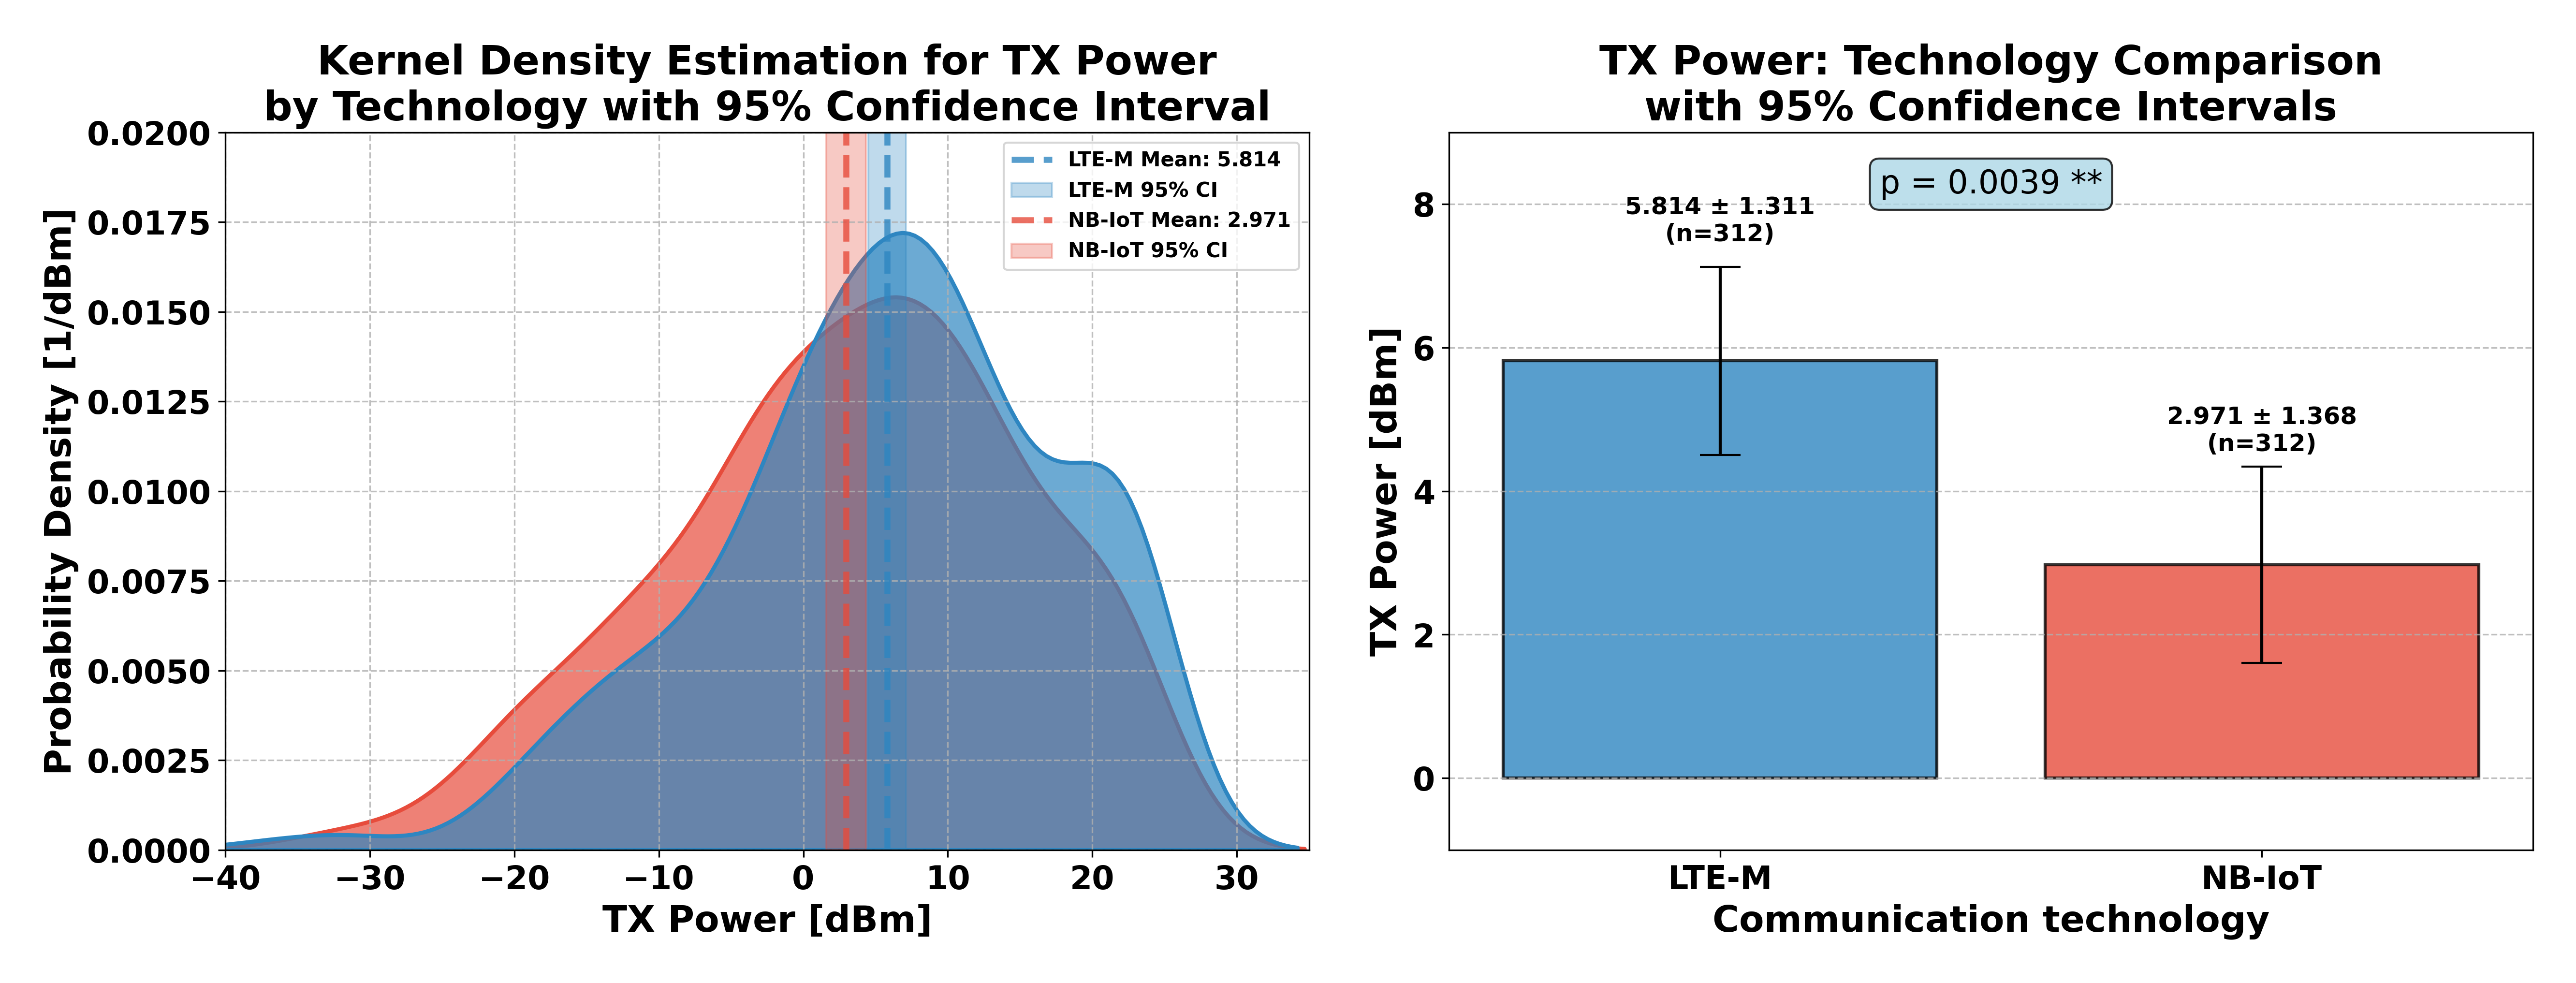
\includegraphics[width=1.0\textwidth]{tx_power_kde_ci.png}
    \caption{\textbf{TX Power Distribution} \\ The figure shows the transmit power distribution for \gls{nbiot} and \gls{ltem} technologies. Lower TX power indicates better energy efficiency and coverage conditions.}
    \label{fig:tx_power}
\end{figure}
\FloatBarrier

\subsubsection*{RSRP Analysis} \label{sec:rsrp_analysis}

The RSRP measurements, visualized in Figure \ref{fig:rsrp} through \gls{kde} and confidence interval plots, demonstrate that \gls{nbiot} achieves a mean \gls{rsrp} approximately 6 dBm higher than \gls{ltem}. Both technologies exhibit comparable variance in their \gls{rsrp} distributions. The statistical analysis using the Mann-Whitney U test returns a p-value of p < 0.001, indicating highly significant evidence that \gls{nbiot} consistently receives stronger reference signal power compared to \gls{ltem} under the measured conditions.

% Figure: RSRP
\begin{figure}[htbp]
    \centering
    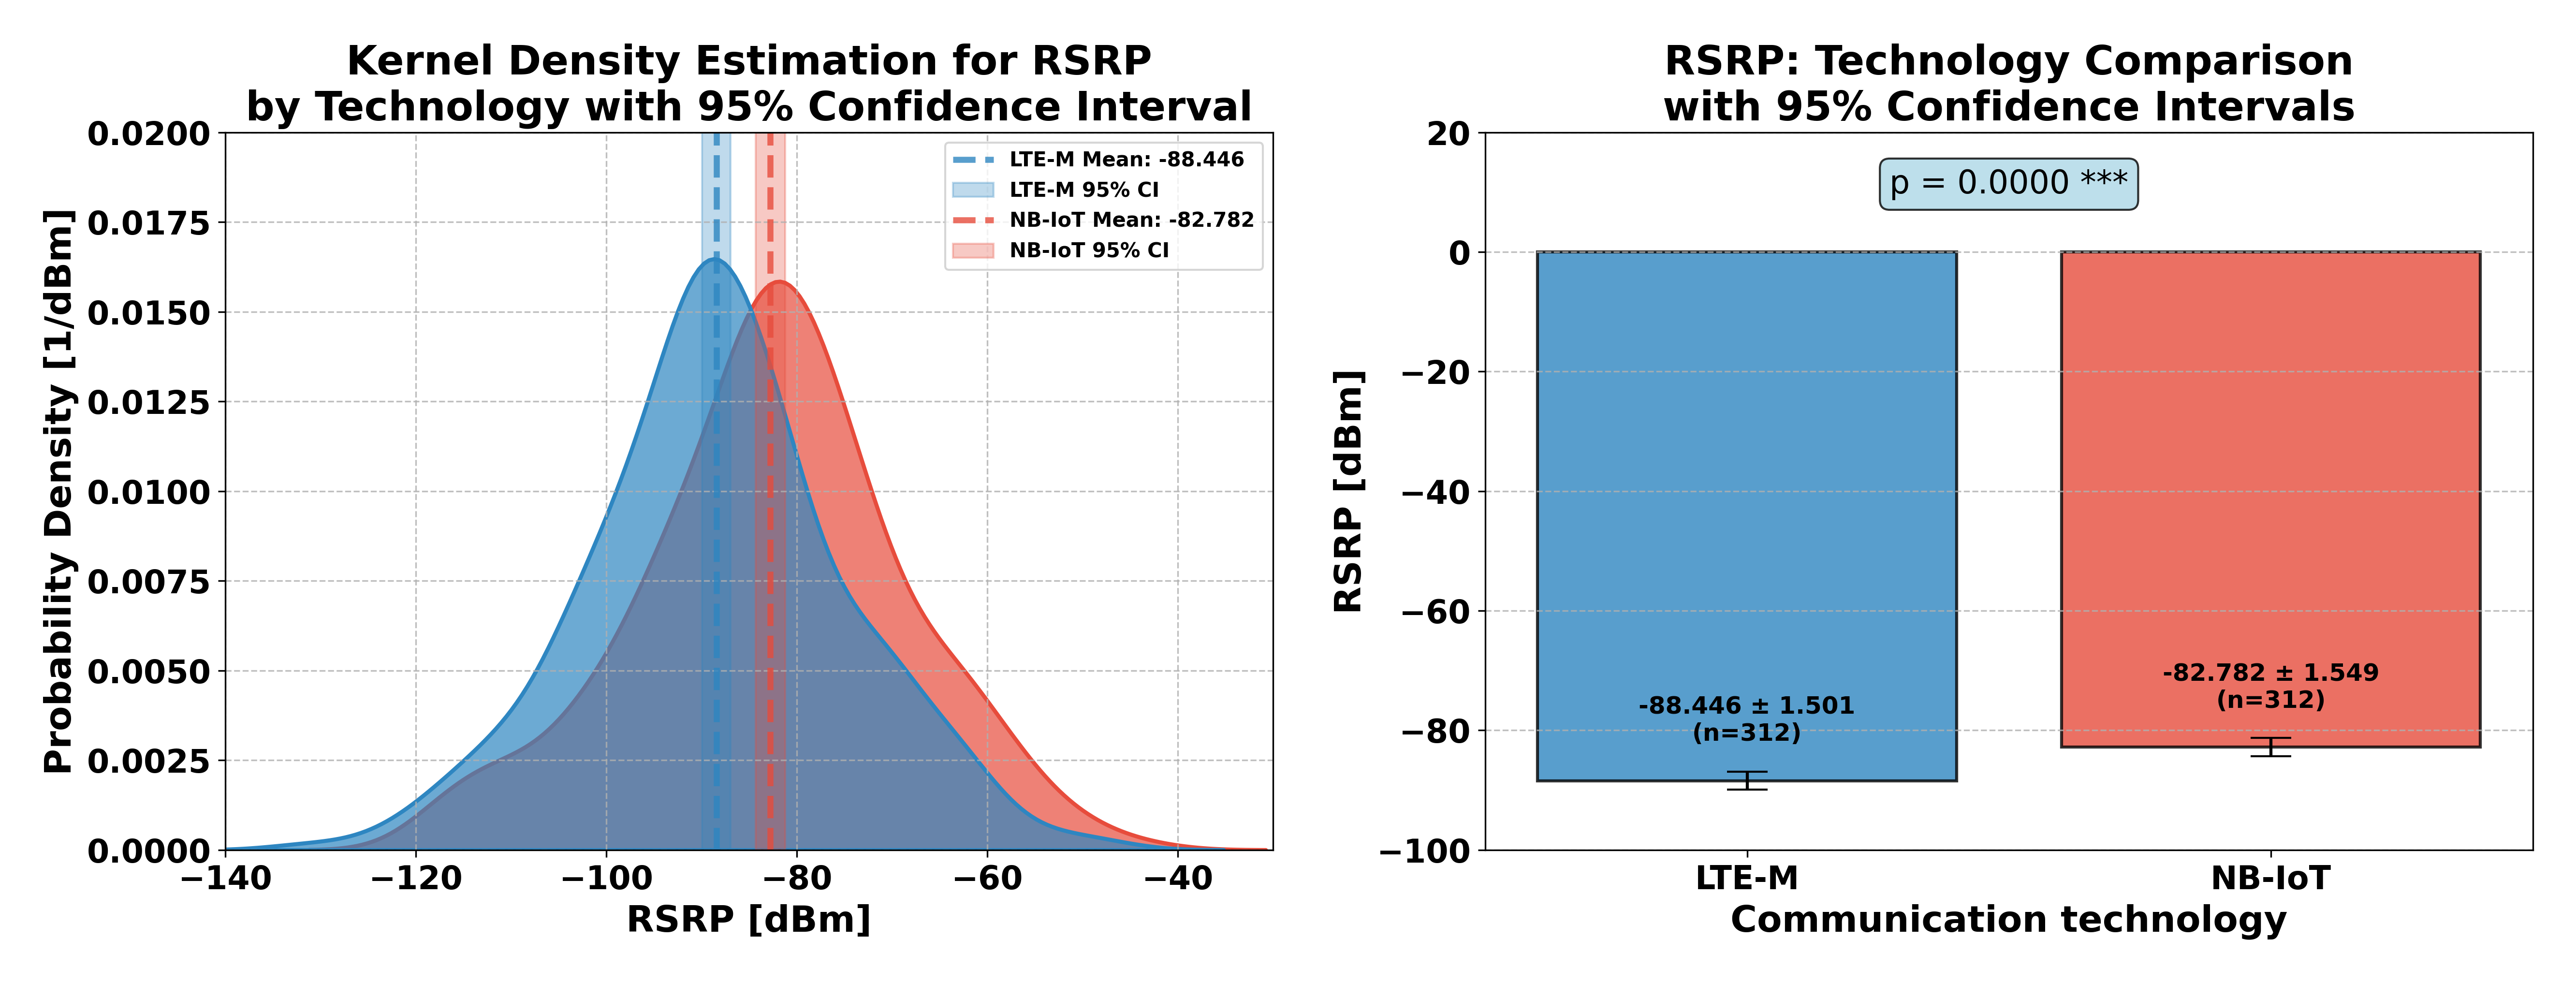
\includegraphics[width=1.0\textwidth]{rsrp_kde_ci.png}
    \caption{\textbf{RSRP Distribution} \\ The figure shows \gls{rsrp} values measured across different locations. Higher \gls{rsrp} values indicate better signal coverage and link quality.}
    \label{fig:rsrp}
\end{figure}
\FloatBarrier
\subsubsection*{RSRQ Analysis} \label{sec:rsrq_analysis}

Figure \ref{fig:rsrq} illustrates the RSRQ distribution comparison, showing that \gls{nbiot} maintains a mean \gls{rsrq} approximately 3.5 dB higher than \gls{ltem}. Notably, \gls{ltem} showed greater variance in \gls{rsrq} measurements compared to \gls{nbiot}, suggesting more variable signal quality conditions. The Mann-Whitney U test produces a p-value of p < 0.001, providing highly significant evidence that \gls{nbiot} delivers superior reference signal quality under the evaluated deployment scenarios.

% Figure: RSRQ
\begin{figure}[htbp]
    \centering
    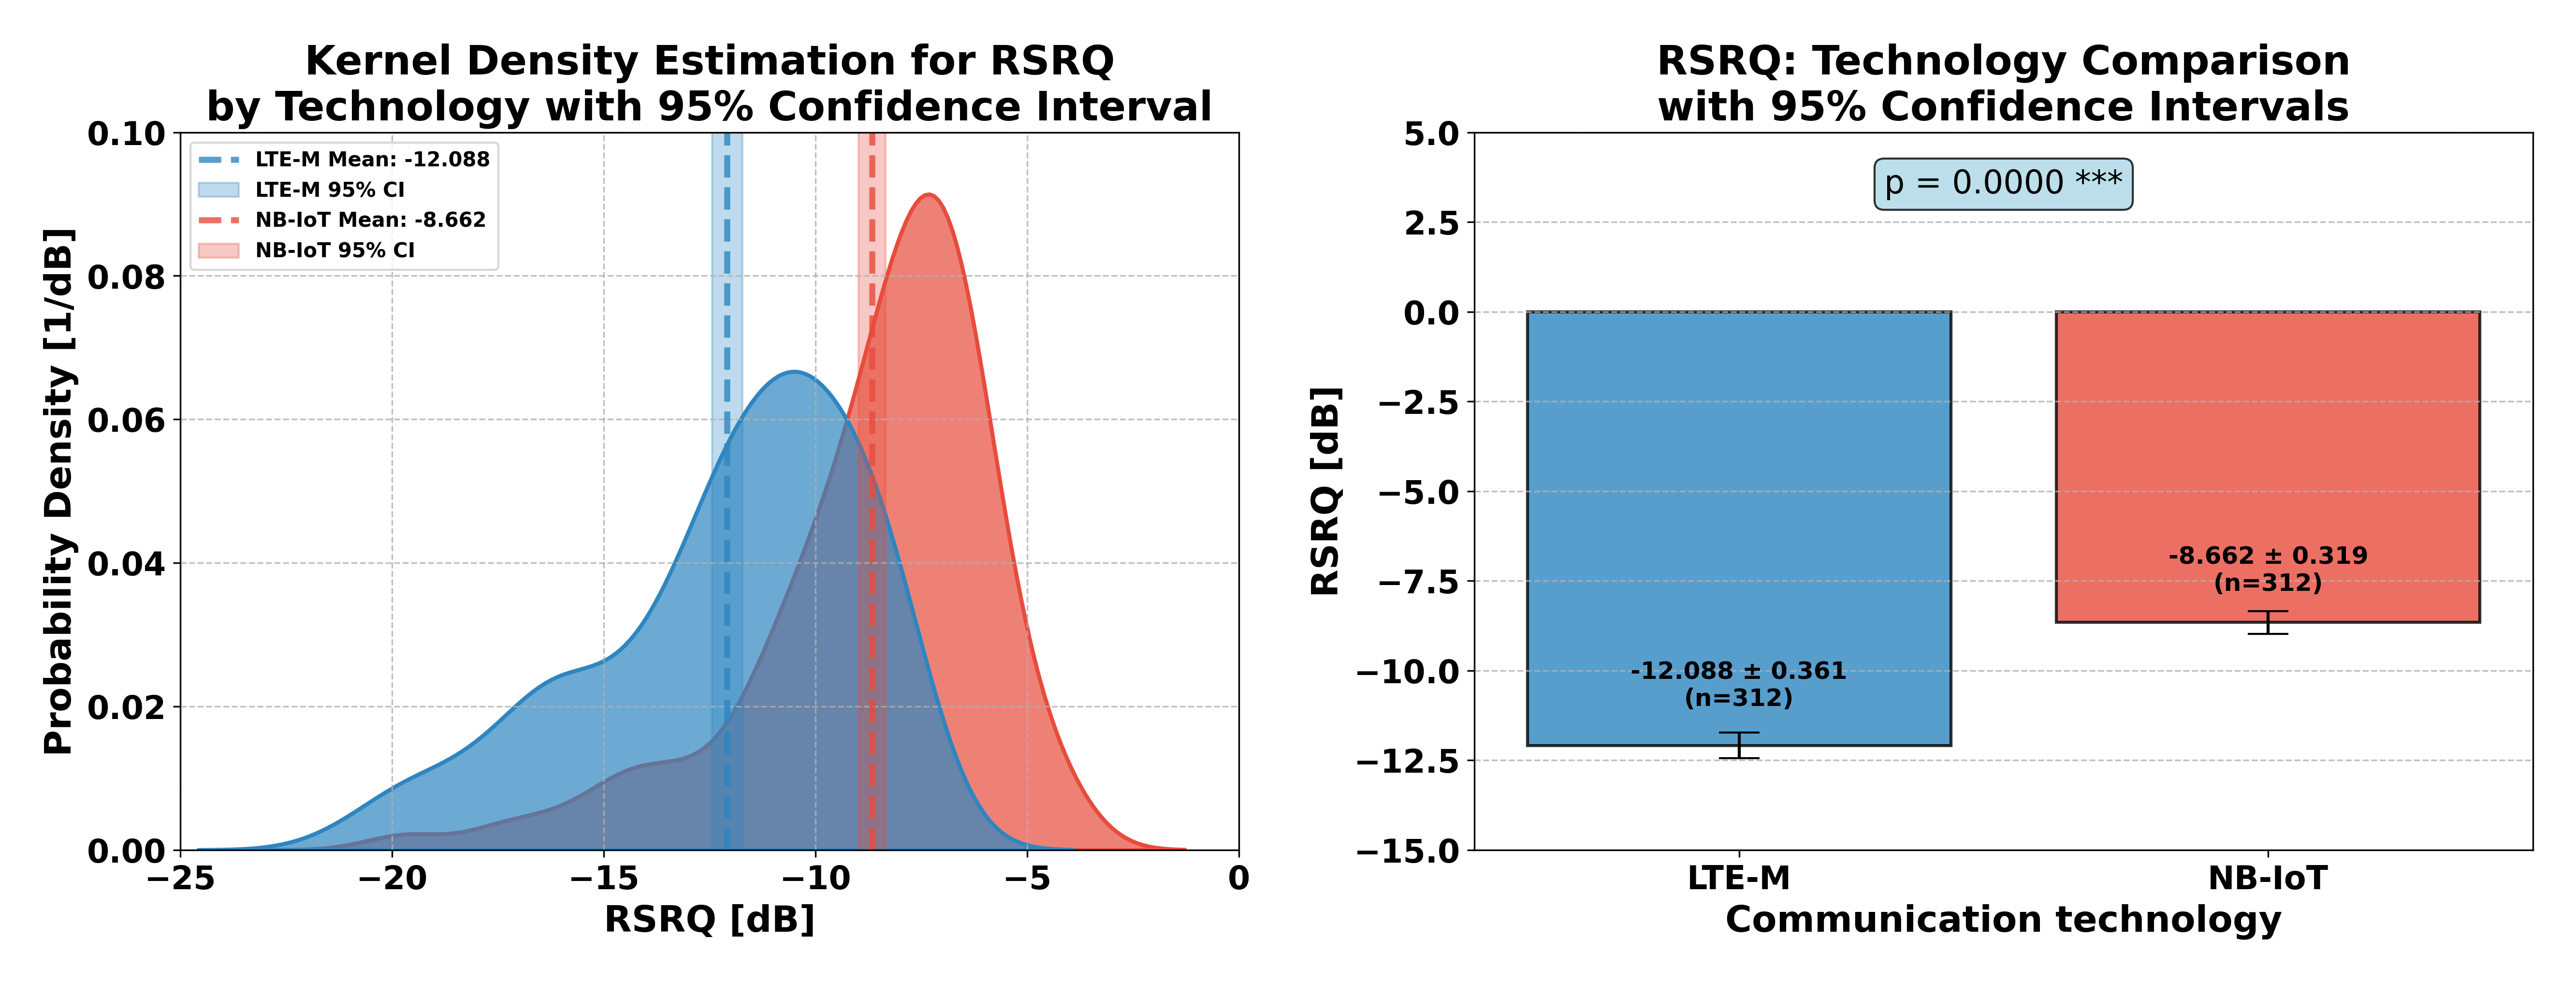
\includegraphics[width=1.0\textwidth]{rsrq_kde_ci.png}
    \caption{\textbf{RSRQ Distribution} \\ The figure shows \gls{rsrq} measurements comparing \gls{nbiot} and \gls{ltem} signal quality. \gls{rsrq} reflects the quality of the received reference signal.}
    \label{fig:rsrq}
\end{figure}
\FloatBarrier
\subsubsection*{SNR Analysis} \label{sec:snr_analysis}

The \gls{snr} distribution analysis, presented in Figure \ref{fig:snr}, reveals that \gls{nbiot} achieves a mean \gls{snr} approximately 3 dB higher than \gls{ltem}. \gls{nbiot} demonstrates greater variance in \gls{snr} measurements compared to \gls{ltem}. Statistical testing using the Mann-Whitney U test yields a p-value of p < 0.001, providing highly significant evidence of superior signal-to-noise performance for \gls{nbiot} technology across the measurement campaign.

% Figure: SNR
\begin{figure}[htbp]
    \centering
    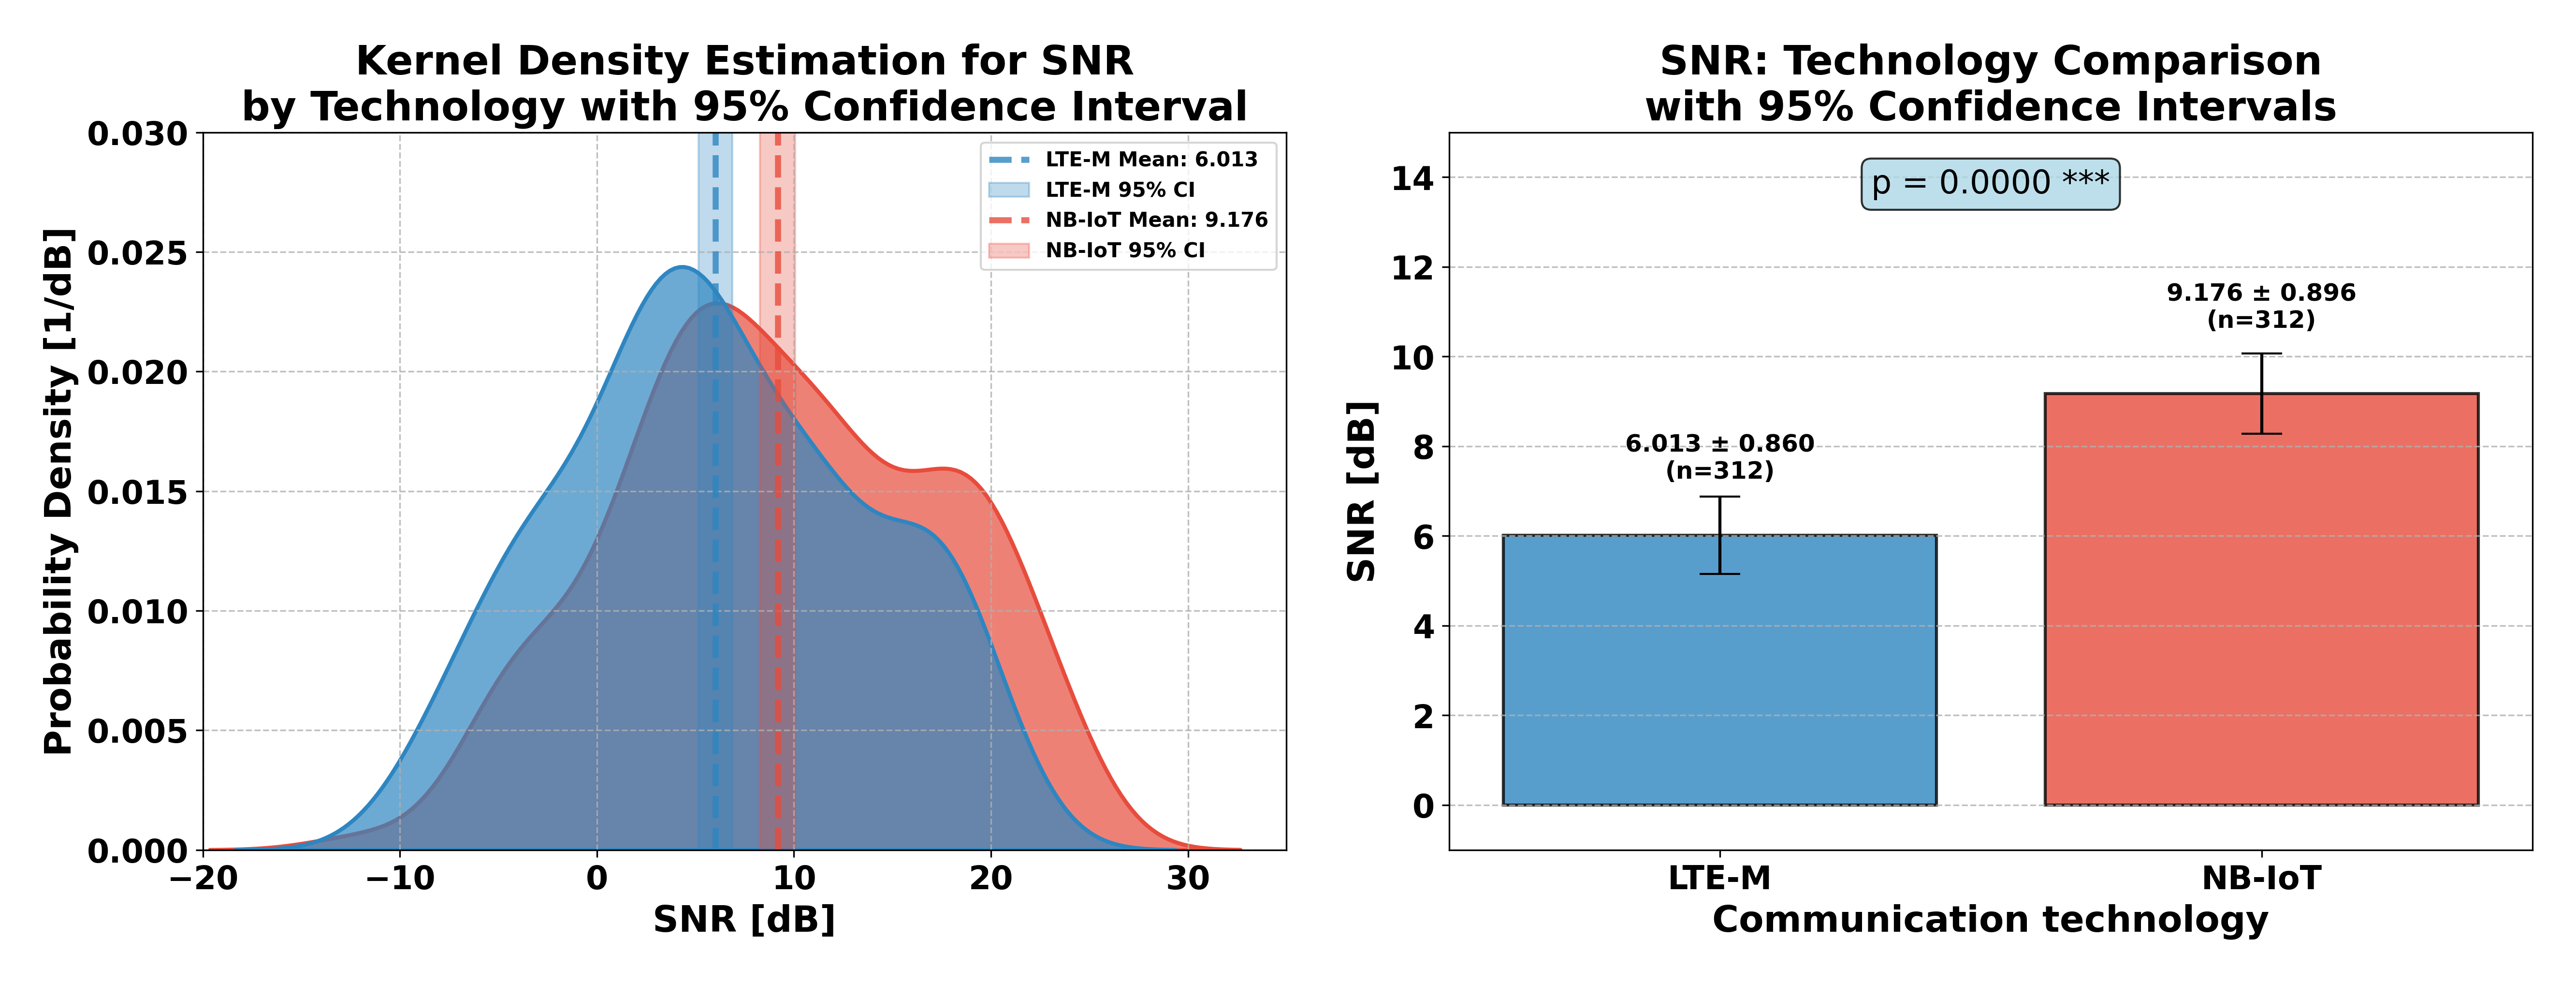
\includegraphics[width=1.0\textwidth]{snr_kde_ci.png}
    \caption{\textbf{SNR Distribution} \\ The figure shows \gls{snr} measurements for both technologies. Higher \gls{snr} values indicate better signal quality and more reliable communication.}
    \label{fig:snr}
\end{figure}
\FloatBarrier
\subsubsection*{Connection Time Analysis} \label{sec:connection_time_analysis}

Figure \ref{fig:connection_time_link} presents the cellular network connection establishment time analysis. The data shows that \gls{nbiot} requires approximately 6.3 seconds longer for network attachment compared to \gls{ltem}. \gls{ltem} demonstrates essential lower variance in connection times, indicating more consistent connection establishment behavior. Statistical analysis using the Mann-Whitney U test confirms highly significant differences (p < 0.001) between the technologies. The presence of outliers, particularly evident in \gls{nbiot} measurements, contributes to the observed higher variance in connection time distributions.

% Figure: Connection Time Link
\begin{figure}[htbp]
    \centering
    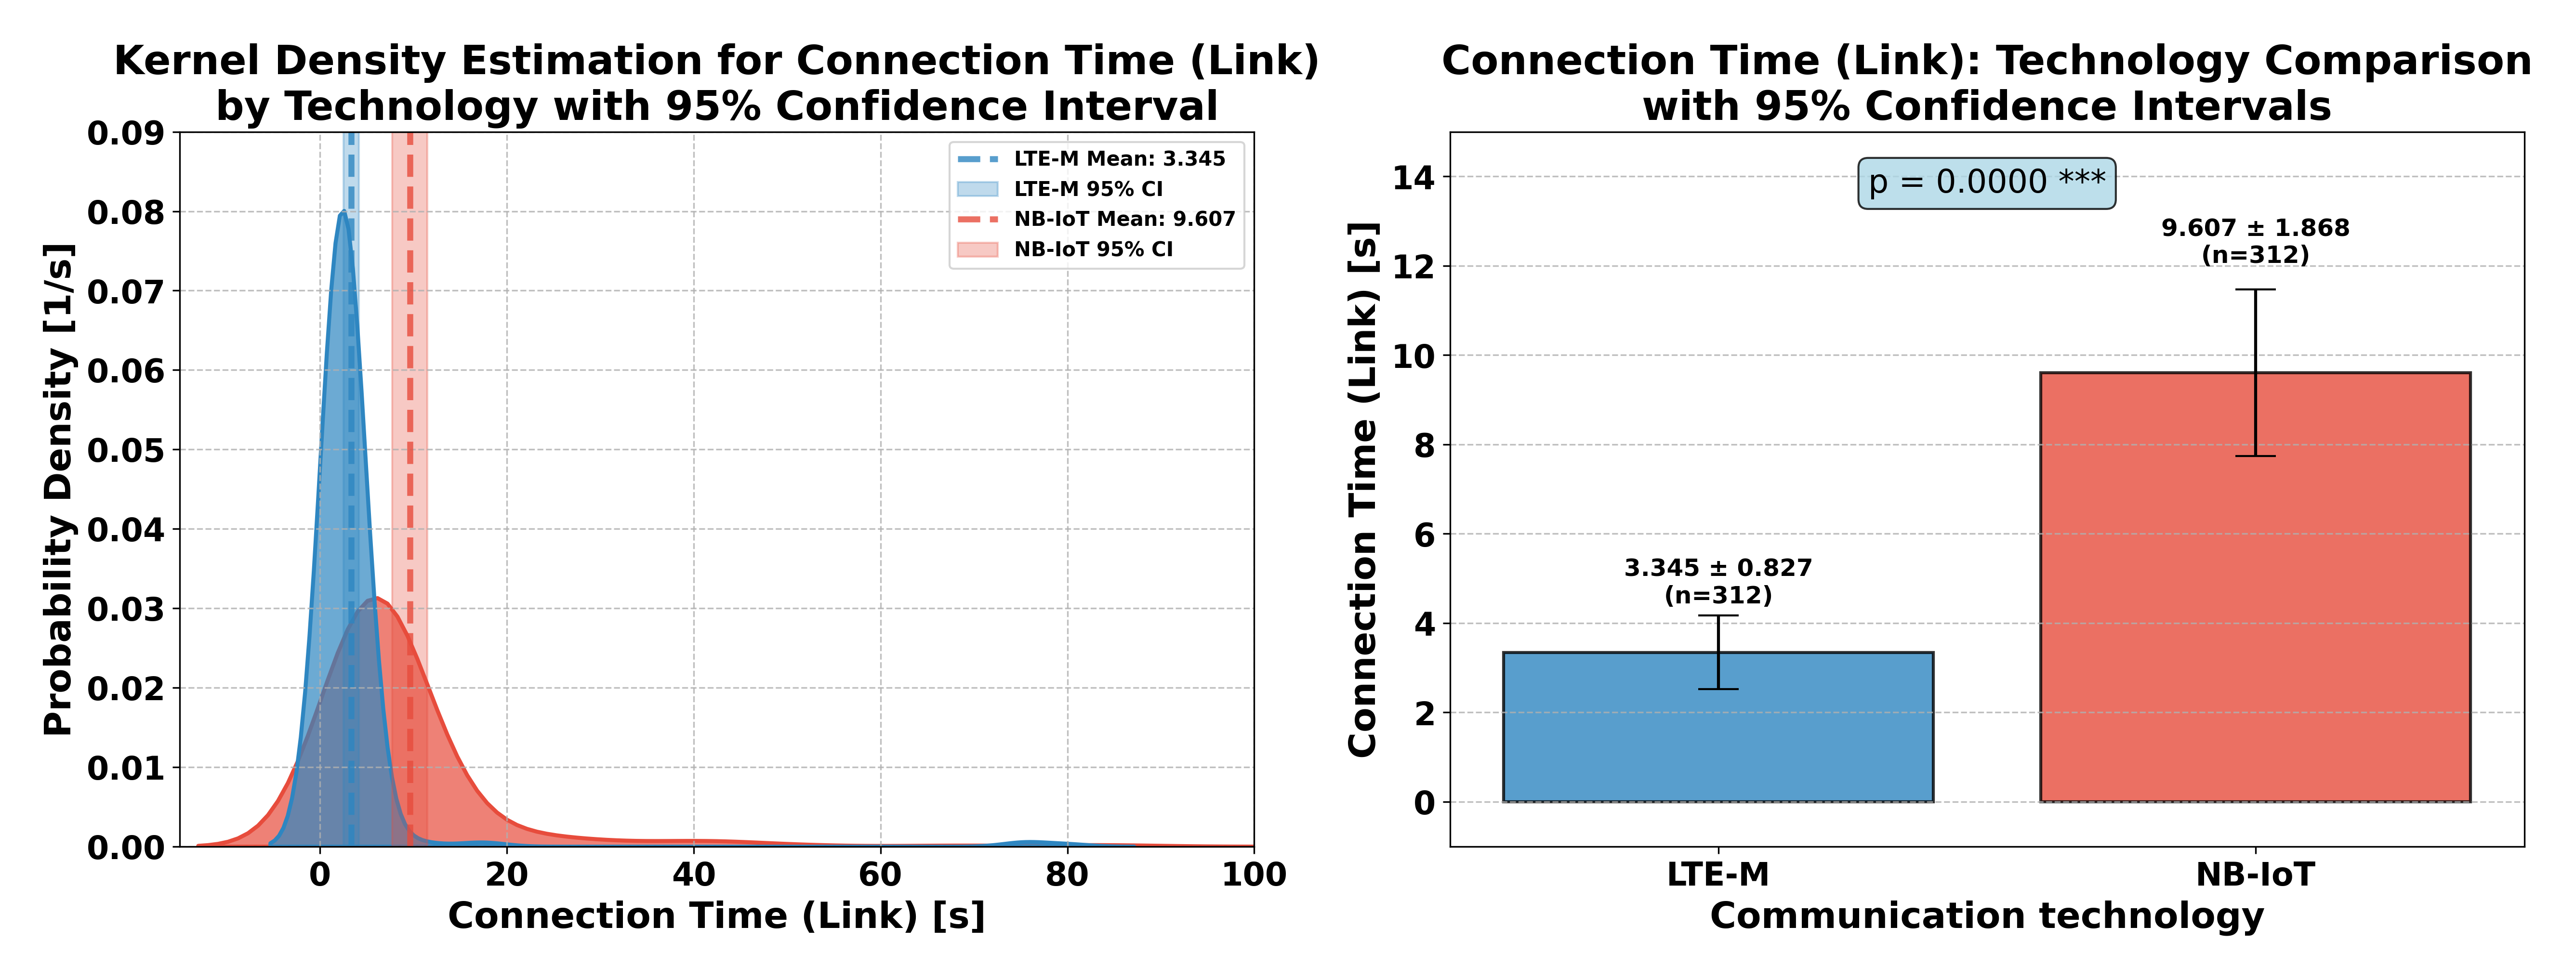
\includegraphics[width=1.0\textwidth]{connection_time_link_kde_ci.png}
    \caption{\textbf{Link Connection Time Distribution} \\ The figure shows the time required to establish cellular network connectivity. Lower connection times indicate faster network attachment and improved user experience.}
    \label{fig:connection_time_link}
\end{figure}
\FloatBarrier
\subsubsection*{Downlink Pathloss Characteristics} \label{sec:downlink_pathloss_analysis}

The downlink pathloss analysis, shown in Figure \ref{fig:downlink_pathloss}, shows minimal differences between technologies. \gls{nbiot} exhibits a mean pathloss 0.4 dB lower than \gls{ltem}, with both technologies demonstrating very similar variance characteristics. The Mann-Whitney U test produces a p-value of 0.608, indicating no statistically significant evidence of pathloss differences between \gls{nbiot} and \gls{ltem} under the measured conditions.

% Figure: Downlink Pathloss
\begin{figure}[htbp]
    \centering
    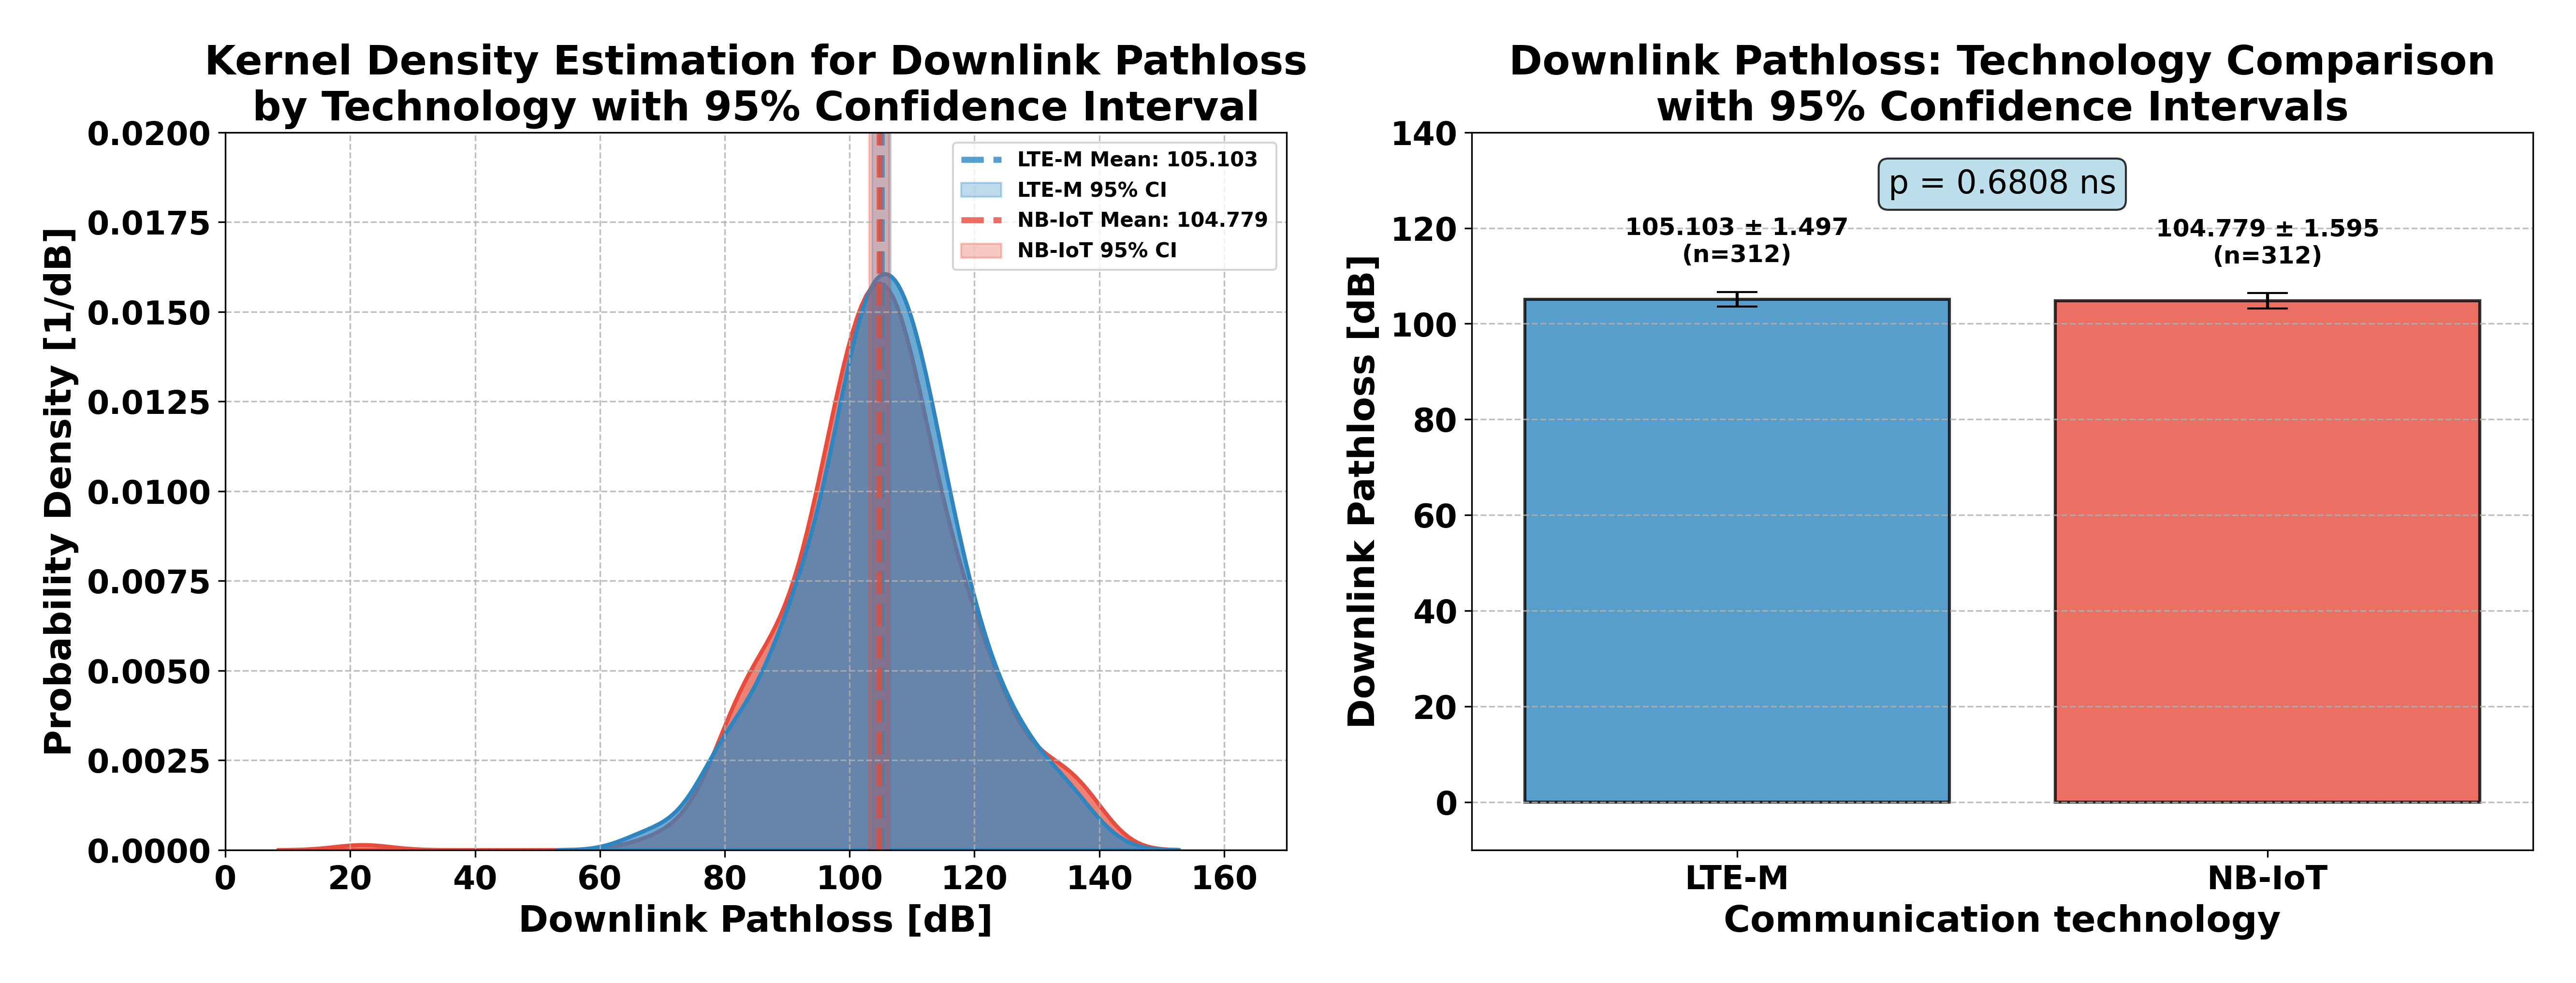
\includegraphics[width=1.0\textwidth]{downlink_pathloss_kde_ci.png}
    \caption{\textbf{Downlink Pathloss Distribution} \\ The figure shows signal attenuation in the downlink path for both \gls{nbiot} and \gls{ltem}. Lower pathloss values indicate better propagation conditions.}
    \label{fig:downlink_pathloss}
\end{figure}
\FloatBarrier
\subsubsection*{Energy Consumption Estimates} \label{sec:energy_consumption_analysis}

Figure \ref{fig:energy_estimate} presents the energy consumption estimate distributions, revealing that \gls{nbiot} shows a mean energy estimate 0.3 units higher than \gls{ltem}. Both technologies have similar variance characteristics. Statistical analysis using the Mann-Whitney U test yields a p-value of 0.0017, providing strong evidence of significant differences in relative energy consumption between the technologies. A notable characteristic observed in both distributions is the discrete pattern with three distinct peaks, reflecting the categorical nature of the energy estimate parameter, which is encoded as discrete integer values by the modem rather than continuous measurements. The observed distribution pattern indicates that both technologies predominantly operate within three specific energy consumption classes, likely corresponding to different coverage enhancement levels or network optimization states implemented by the cellular operator.

% Figure: Energy Estimate
\begin{figure}[htbp]
    \centering
    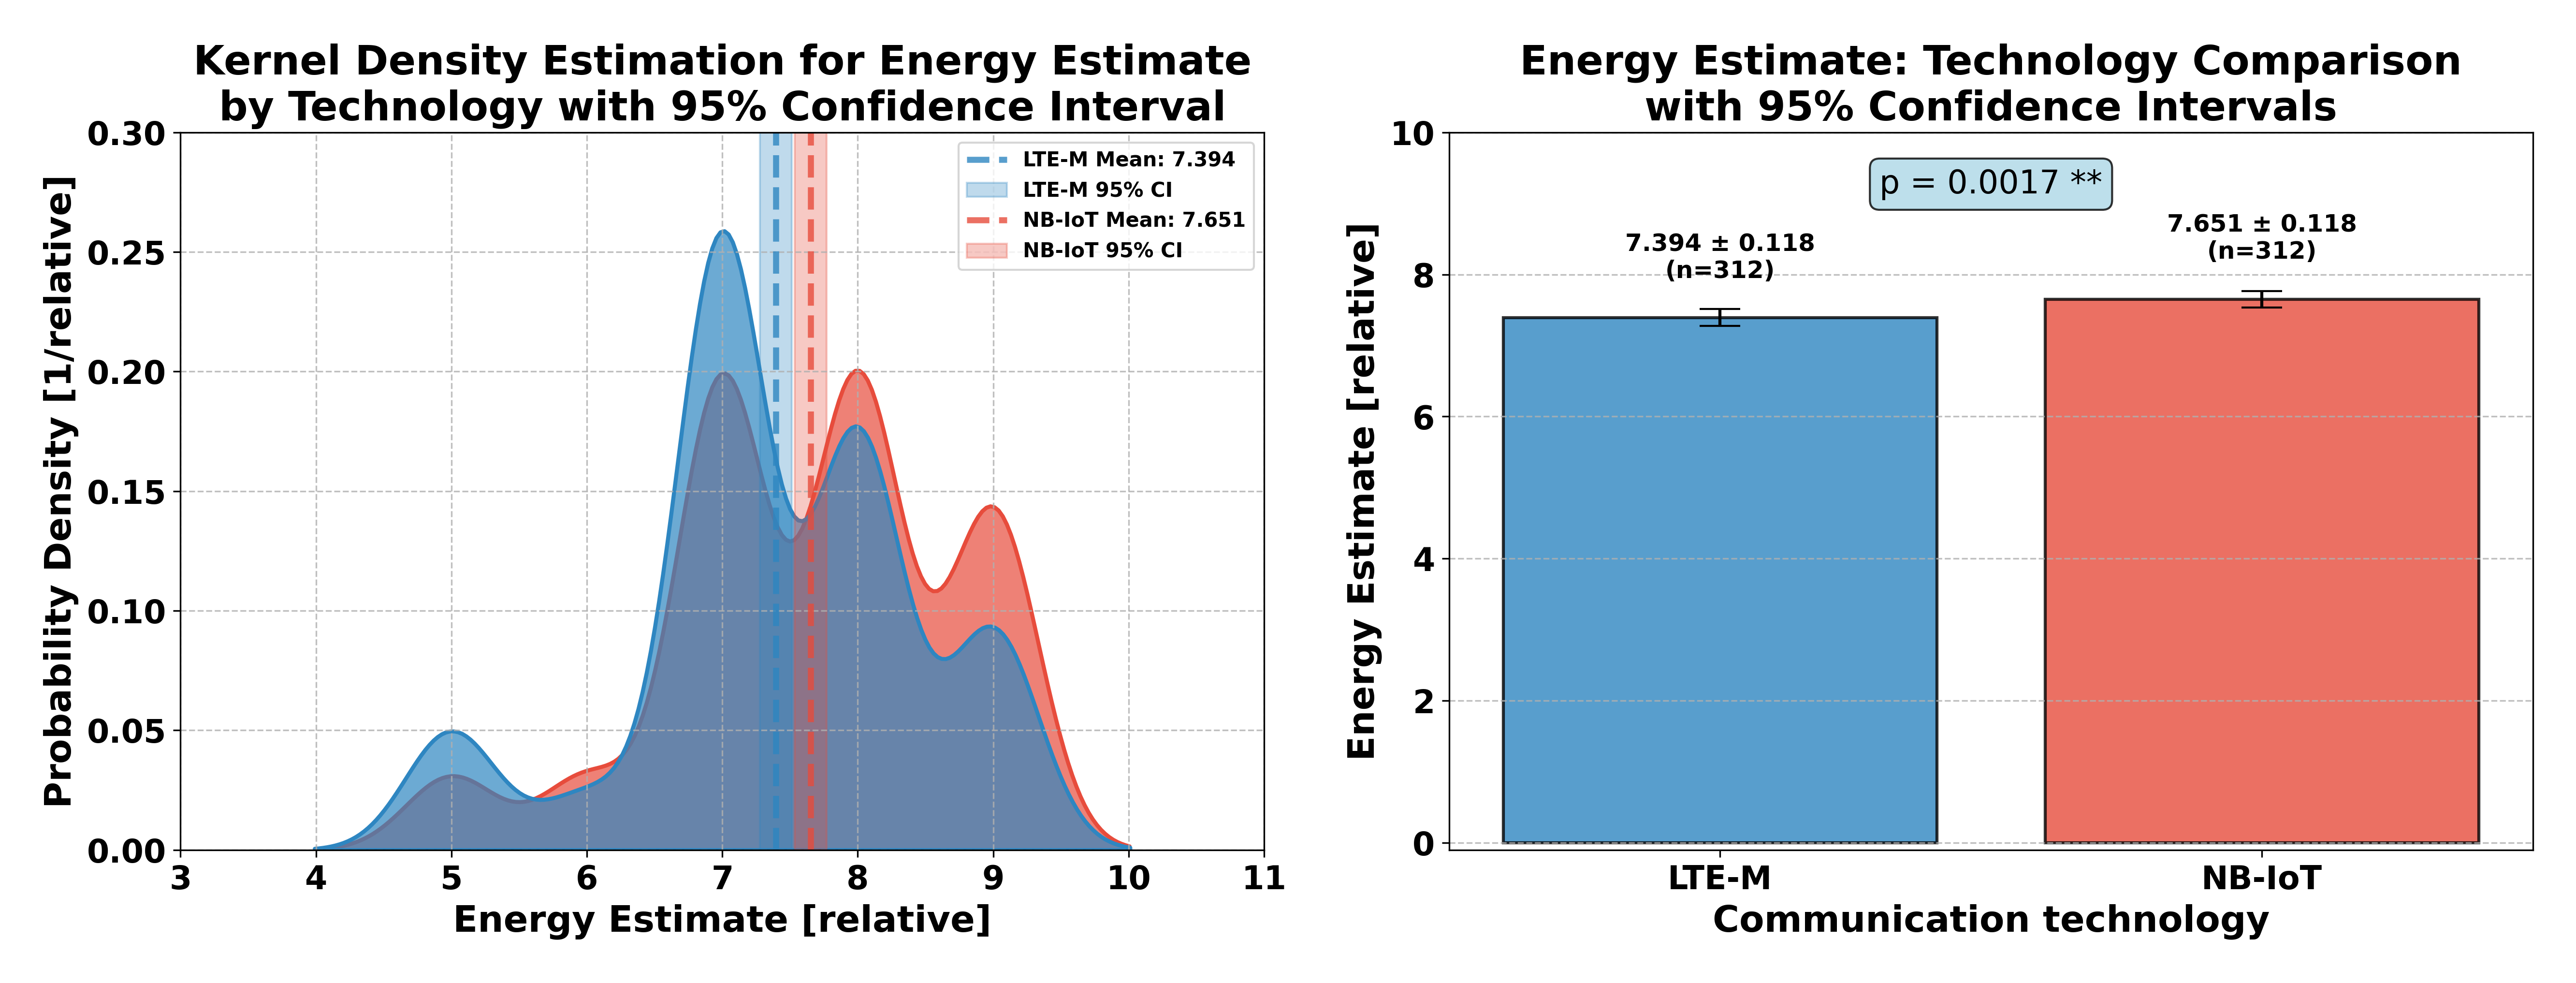
\includegraphics[width=1.0\textwidth]{energy_estimate_kde_ci.png}
    \caption{\textbf{Energy Estimate Distribution} \\ The figure shows relative energy consumption estimates for data transmission. Lower values indicate more energy-efficient communication.}
    \label{fig:energy_estimate}
\end{figure}
\FloatBarrier
\subsubsection*{Receive Repetitions Analysis}\label{sec:receive_repetitions_analysis}

The receive repetitions analysis, shown in Figure \ref{fig:rx_repetitions}, indicates that \gls{nbiot} requires 0.3 counts fewer receive repetitions than \gls{ltem} on average. \gls{ltem} demonstrates higher variance in repetition requirements compared to \gls{nbiot}. The Mann-Whitney U test produces a p-value of 0.25, indicating insufficient evidence to conclude significant differences in receive repetition requirements between the technologies.

% Figure: RX Repetitions
\begin{figure}[htbp]
    \centering
    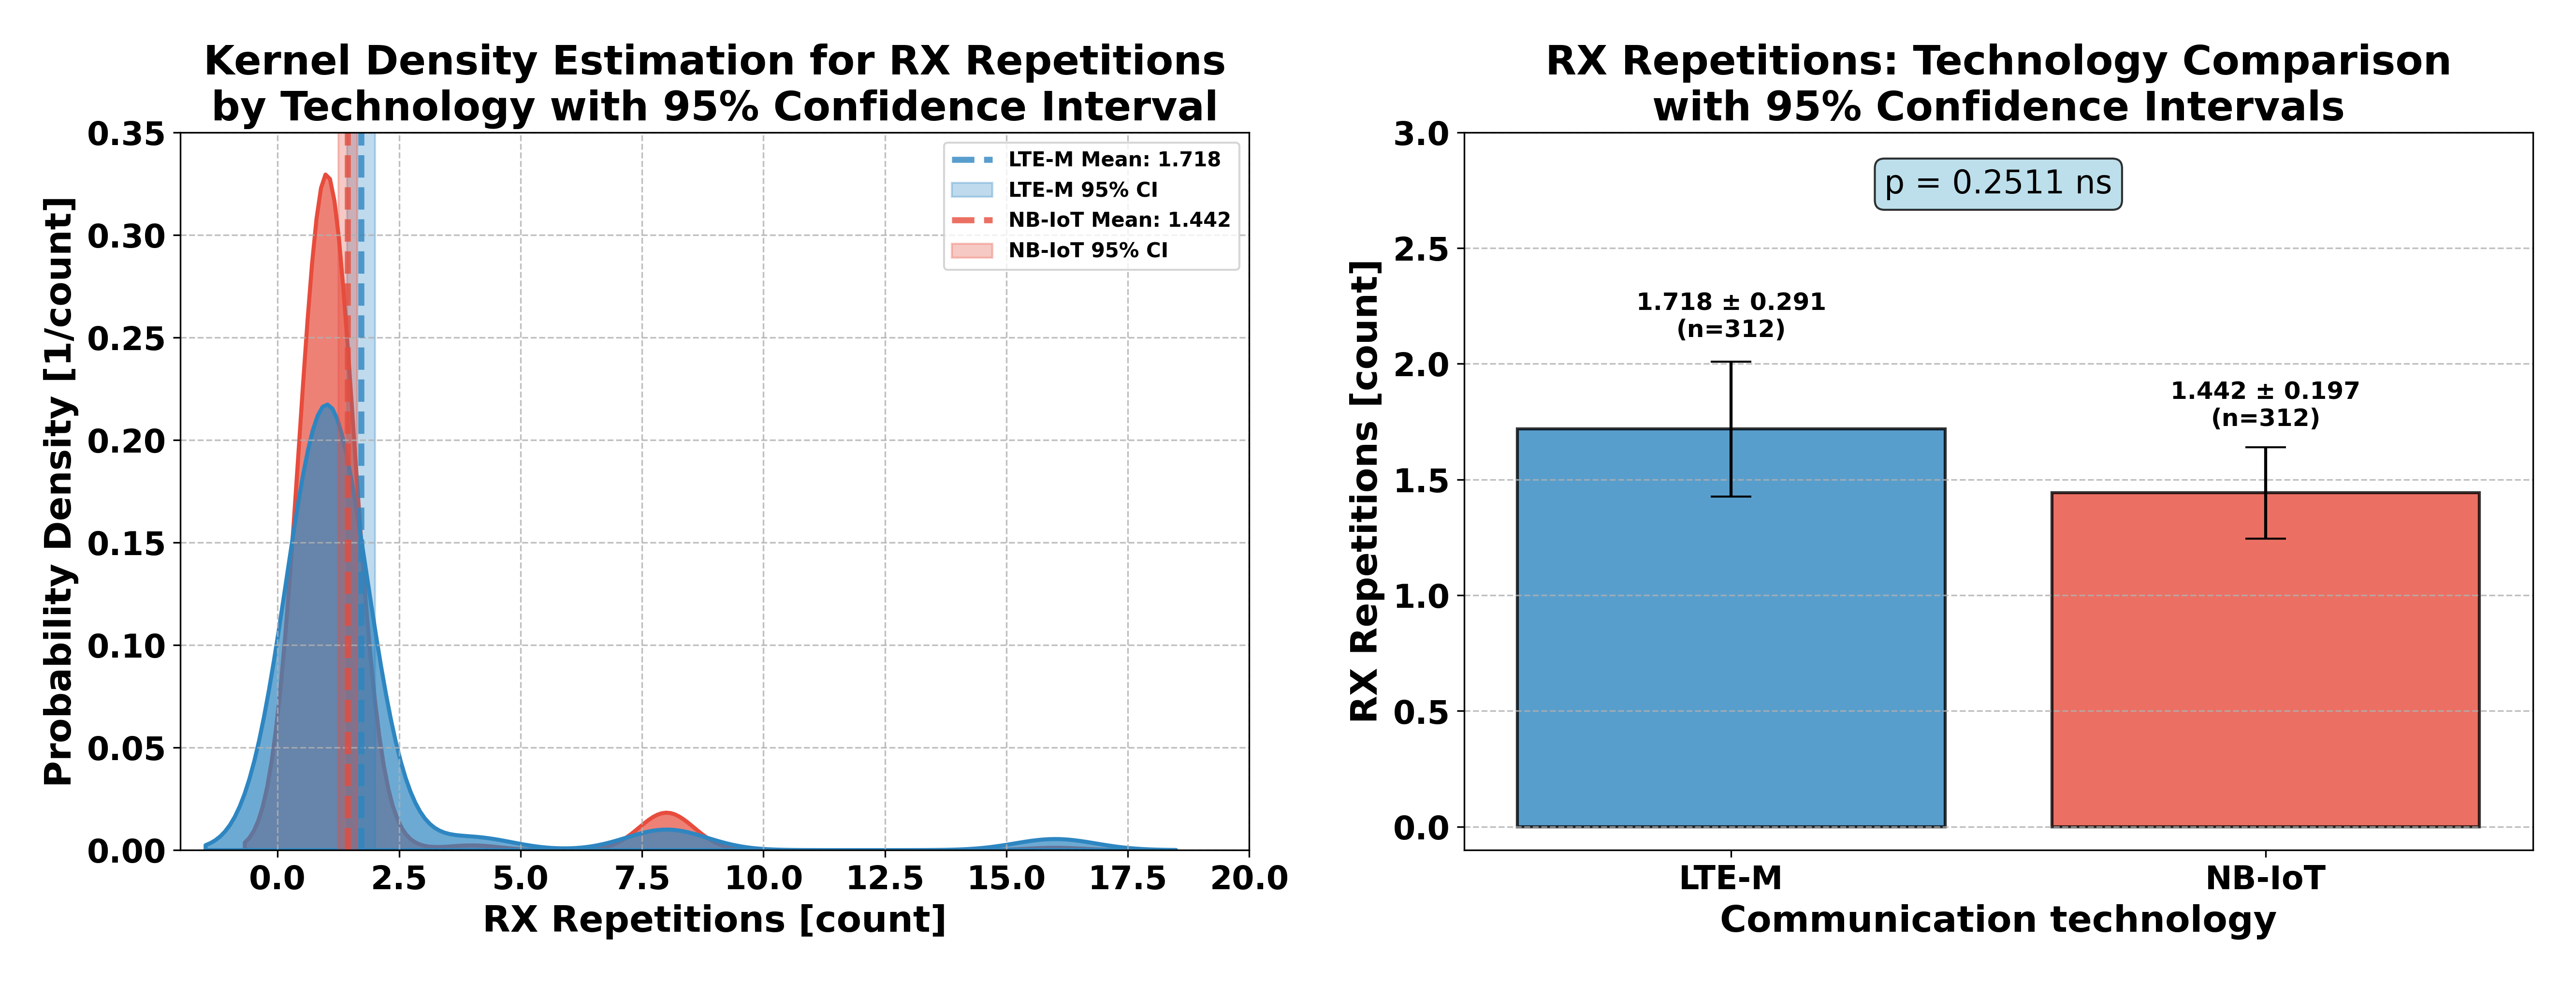
\includegraphics[width=1.0\textwidth]{rx_repetitions_kde_ci.png}
    \caption{\textbf{RX Repetitions Distribution} \\ The figure shows the number of receive repetitions required for reliable communication. Higher repetitions indicate poorer link conditions.}
    \label{fig:rx_repetitions}
\end{figure}
\FloatBarrier
\subsubsection*{Transmit Repetitions Analysis} \label{sec:transmit_repetitions_analysis}

Figure \ref{fig:tx_repetitions} presents the transmit repetitions comparison, showing that \gls{nbiot} requires approximately 0.6 counts more transmit repetitions than \gls{ltem} on average. \gls{nbiot} exhibits greater variance and the presence of outliers in transmission repetition requirements. Statistical analysis using the Mann-Whitney U test yields a p-value of p < 0.001, providing highly significant evidence that \gls{nbiot} requires more transmission repetitions for reliable uplink communication compared to \gls{ltem}.

% Figure: TX Repetitions
\begin{figure}[htbp]
    \centering
    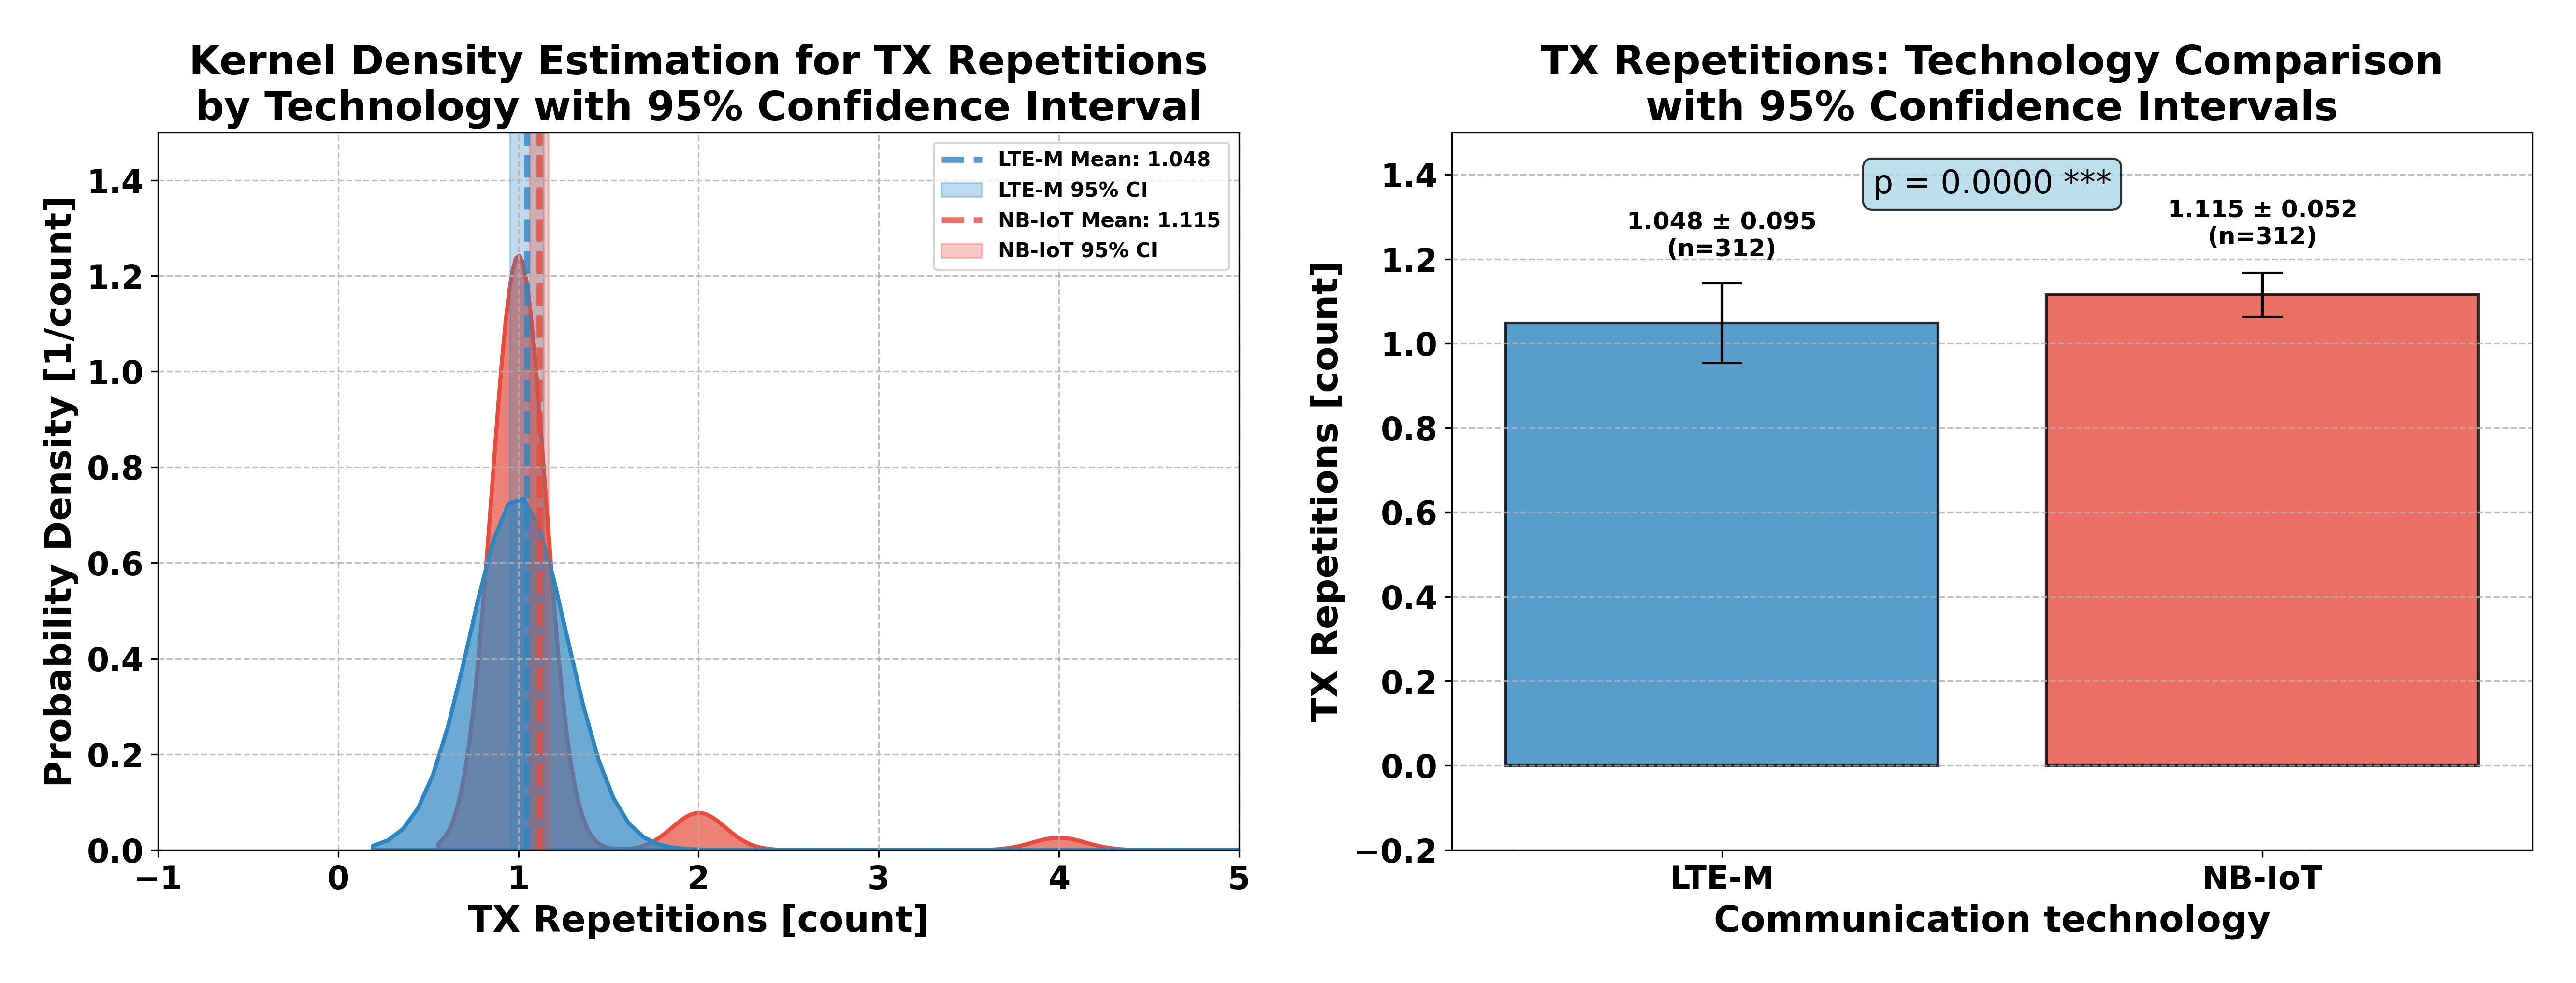
\includegraphics[width=1.0\textwidth]{tx_repetitions_kde_ci.png}
    \caption{\textbf{TX Repetitions Distribution} \\ The figure shows the number of transmission repetitions required for reliable uplink communication. Higher repetitions indicate coverage enhancement needs.}
    \label{fig:tx_repetitions}
\end{figure}
\FloatBarrier
\subsubsection*{Link Throughput Performance} \label{sec:link_throughput_analysis}

The uplink throughput analysis, presented in Figure \ref{fig:throughput_link}, reveals substantial differences between technologies. The measurement employed a UDP-based two-packet timing method where the device transmitted a 512-byte payload to a remote server, with throughput calculated based on precise kernel timestamps and total packet size including protocol headers (554 bytes total). \gls{nbiot} achieves approximately 215 kbps lower uplink throughput than \gls{ltem} on average. \gls{ltem} demonstrates significantly higher variance in uplink throughput measurements. Statistical testing using the Mann-Whitney U test confirms highly significant differences (p < 0.001) between the technologies. The uplink data shows \gls{nbiot} throughput consistently ranges between 0-100 kbps, while \gls{ltem} has a peak around 300 kbps with a broad uplink distribution spanning 100-380 kbps. These uplink throughput characteristics directly impact the data transmission capabilities for outdoor sensor deployments, where sensor data must be efficiently transmitted from field devices to remote monitoring systems.

% Figure: Throughput Link
\begin{figure}[htbp]
    \centering
    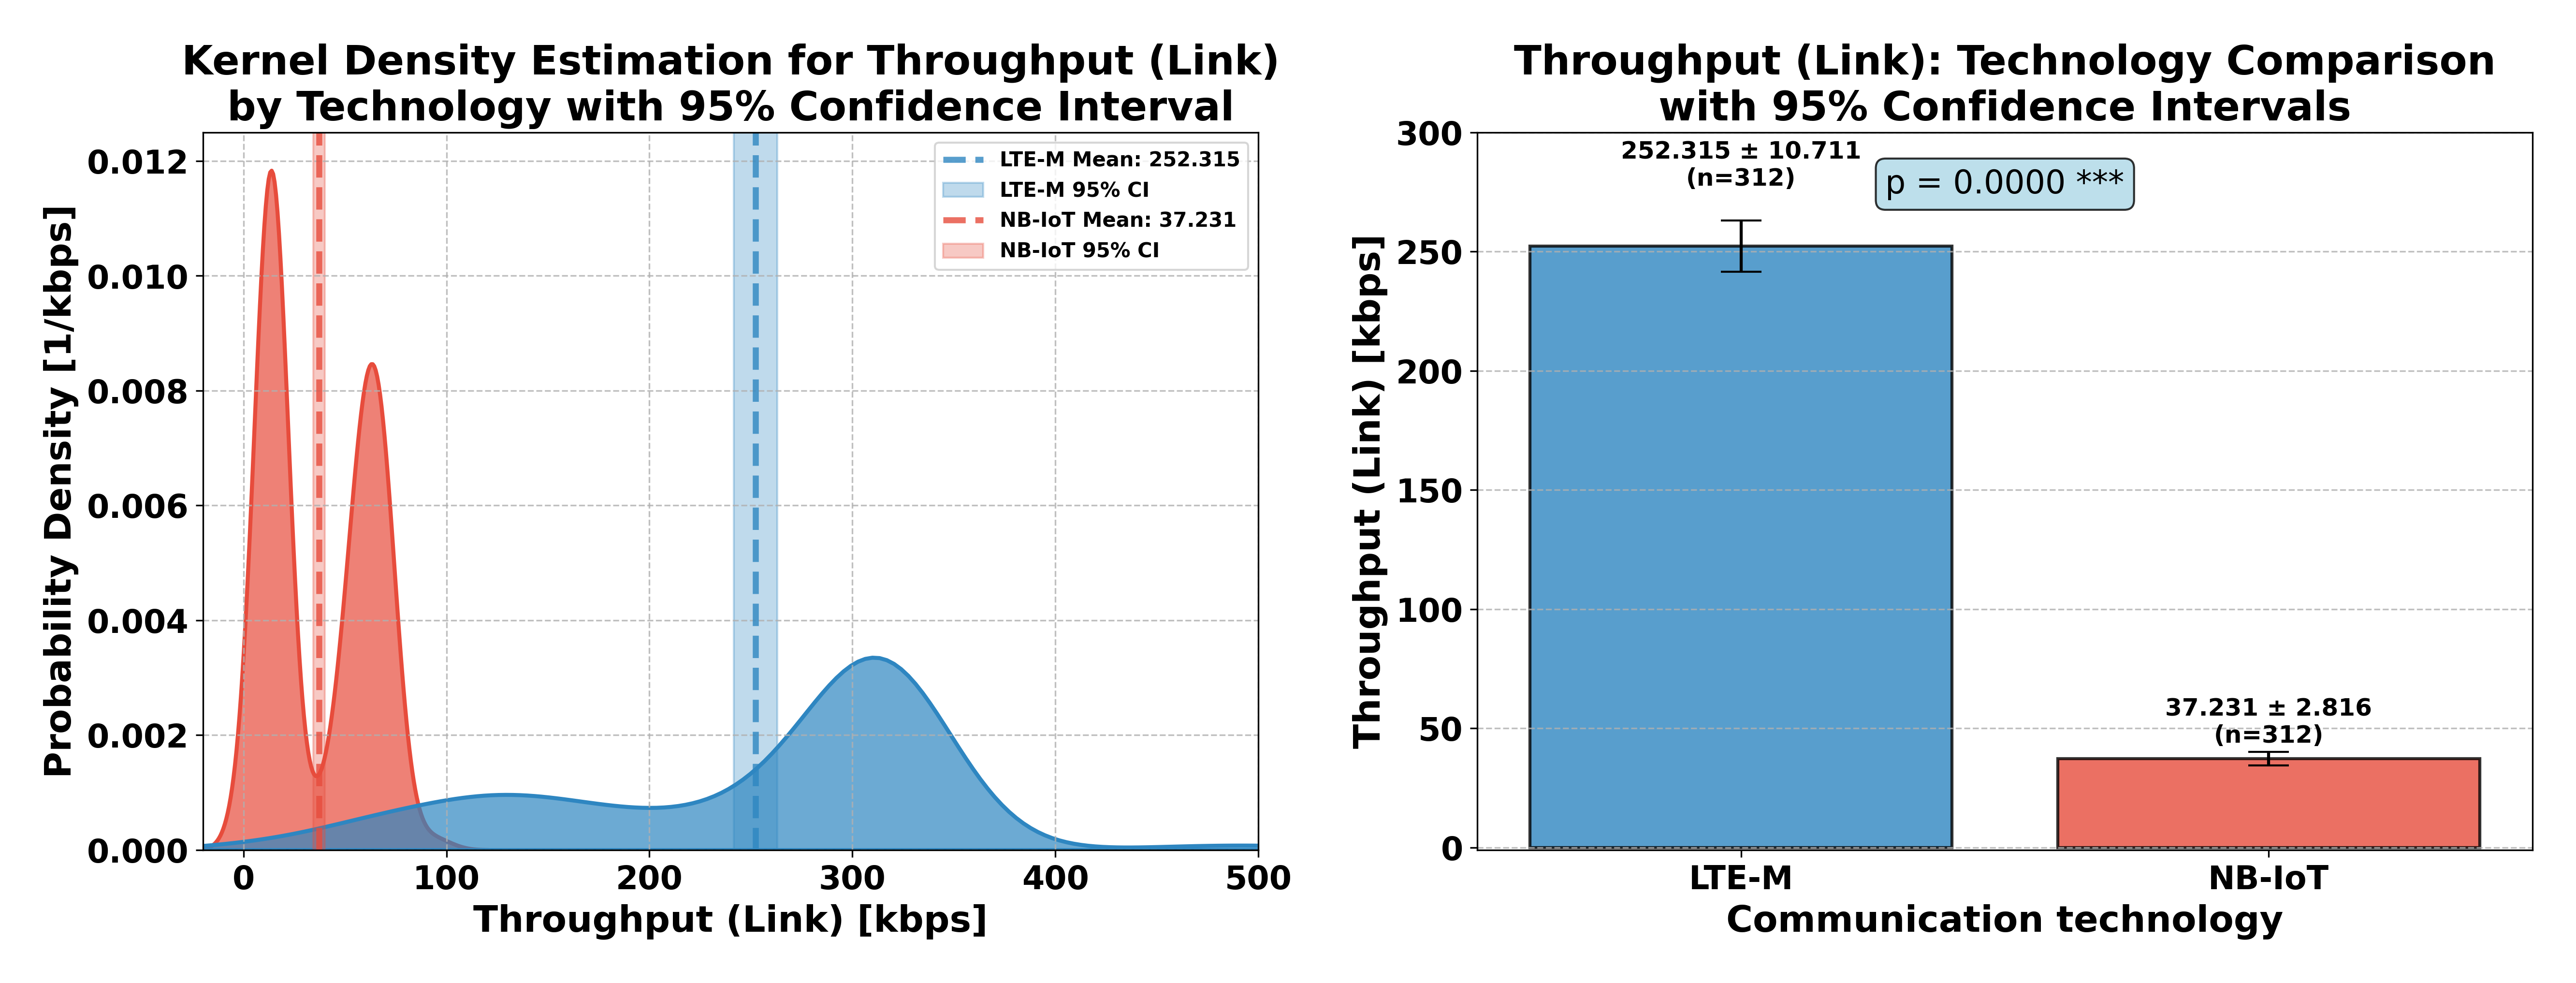
\includegraphics[width=1.0\textwidth]{throughput_link_kde_ci.png}
    \caption{\textbf{Link Throughput Distribution} \\ The figure shows achieved data throughput for \gls{nbiot} and \gls{ltem} connections. Higher throughput values indicate better data transmission performance.}
    \label{fig:throughput_link}
\end{figure}
\FloatBarrier
\subsubsection*{Uplink Frequency Analysis} \label{sec:uplink_frequency_analysis}

Figure \ref{fig:uplink_frequency} illustrates the uplink frequency distribution, showing that \gls{ltem} operates across two primary frequency bands: Band 20 (832-862 MHz) and Band 3 (1710-1785 MHz). \gls{nbiot} utilizes Band 8 (880-915 MHz) and Band 20 (832-862 MHz). \gls{nbiot} demonstrates lower variance in frequency utilization compared to \gls{ltem}, indicating more constrained frequency band deployment. Both technologies share Band 20 for uplink transmission, while \gls{ltem} additionally utilizes the higher frequency Band 3 and \gls{nbiot} uses Band 8.

% Figure: Uplink Frequency
\begin{figure}[htbp]
    \centering
    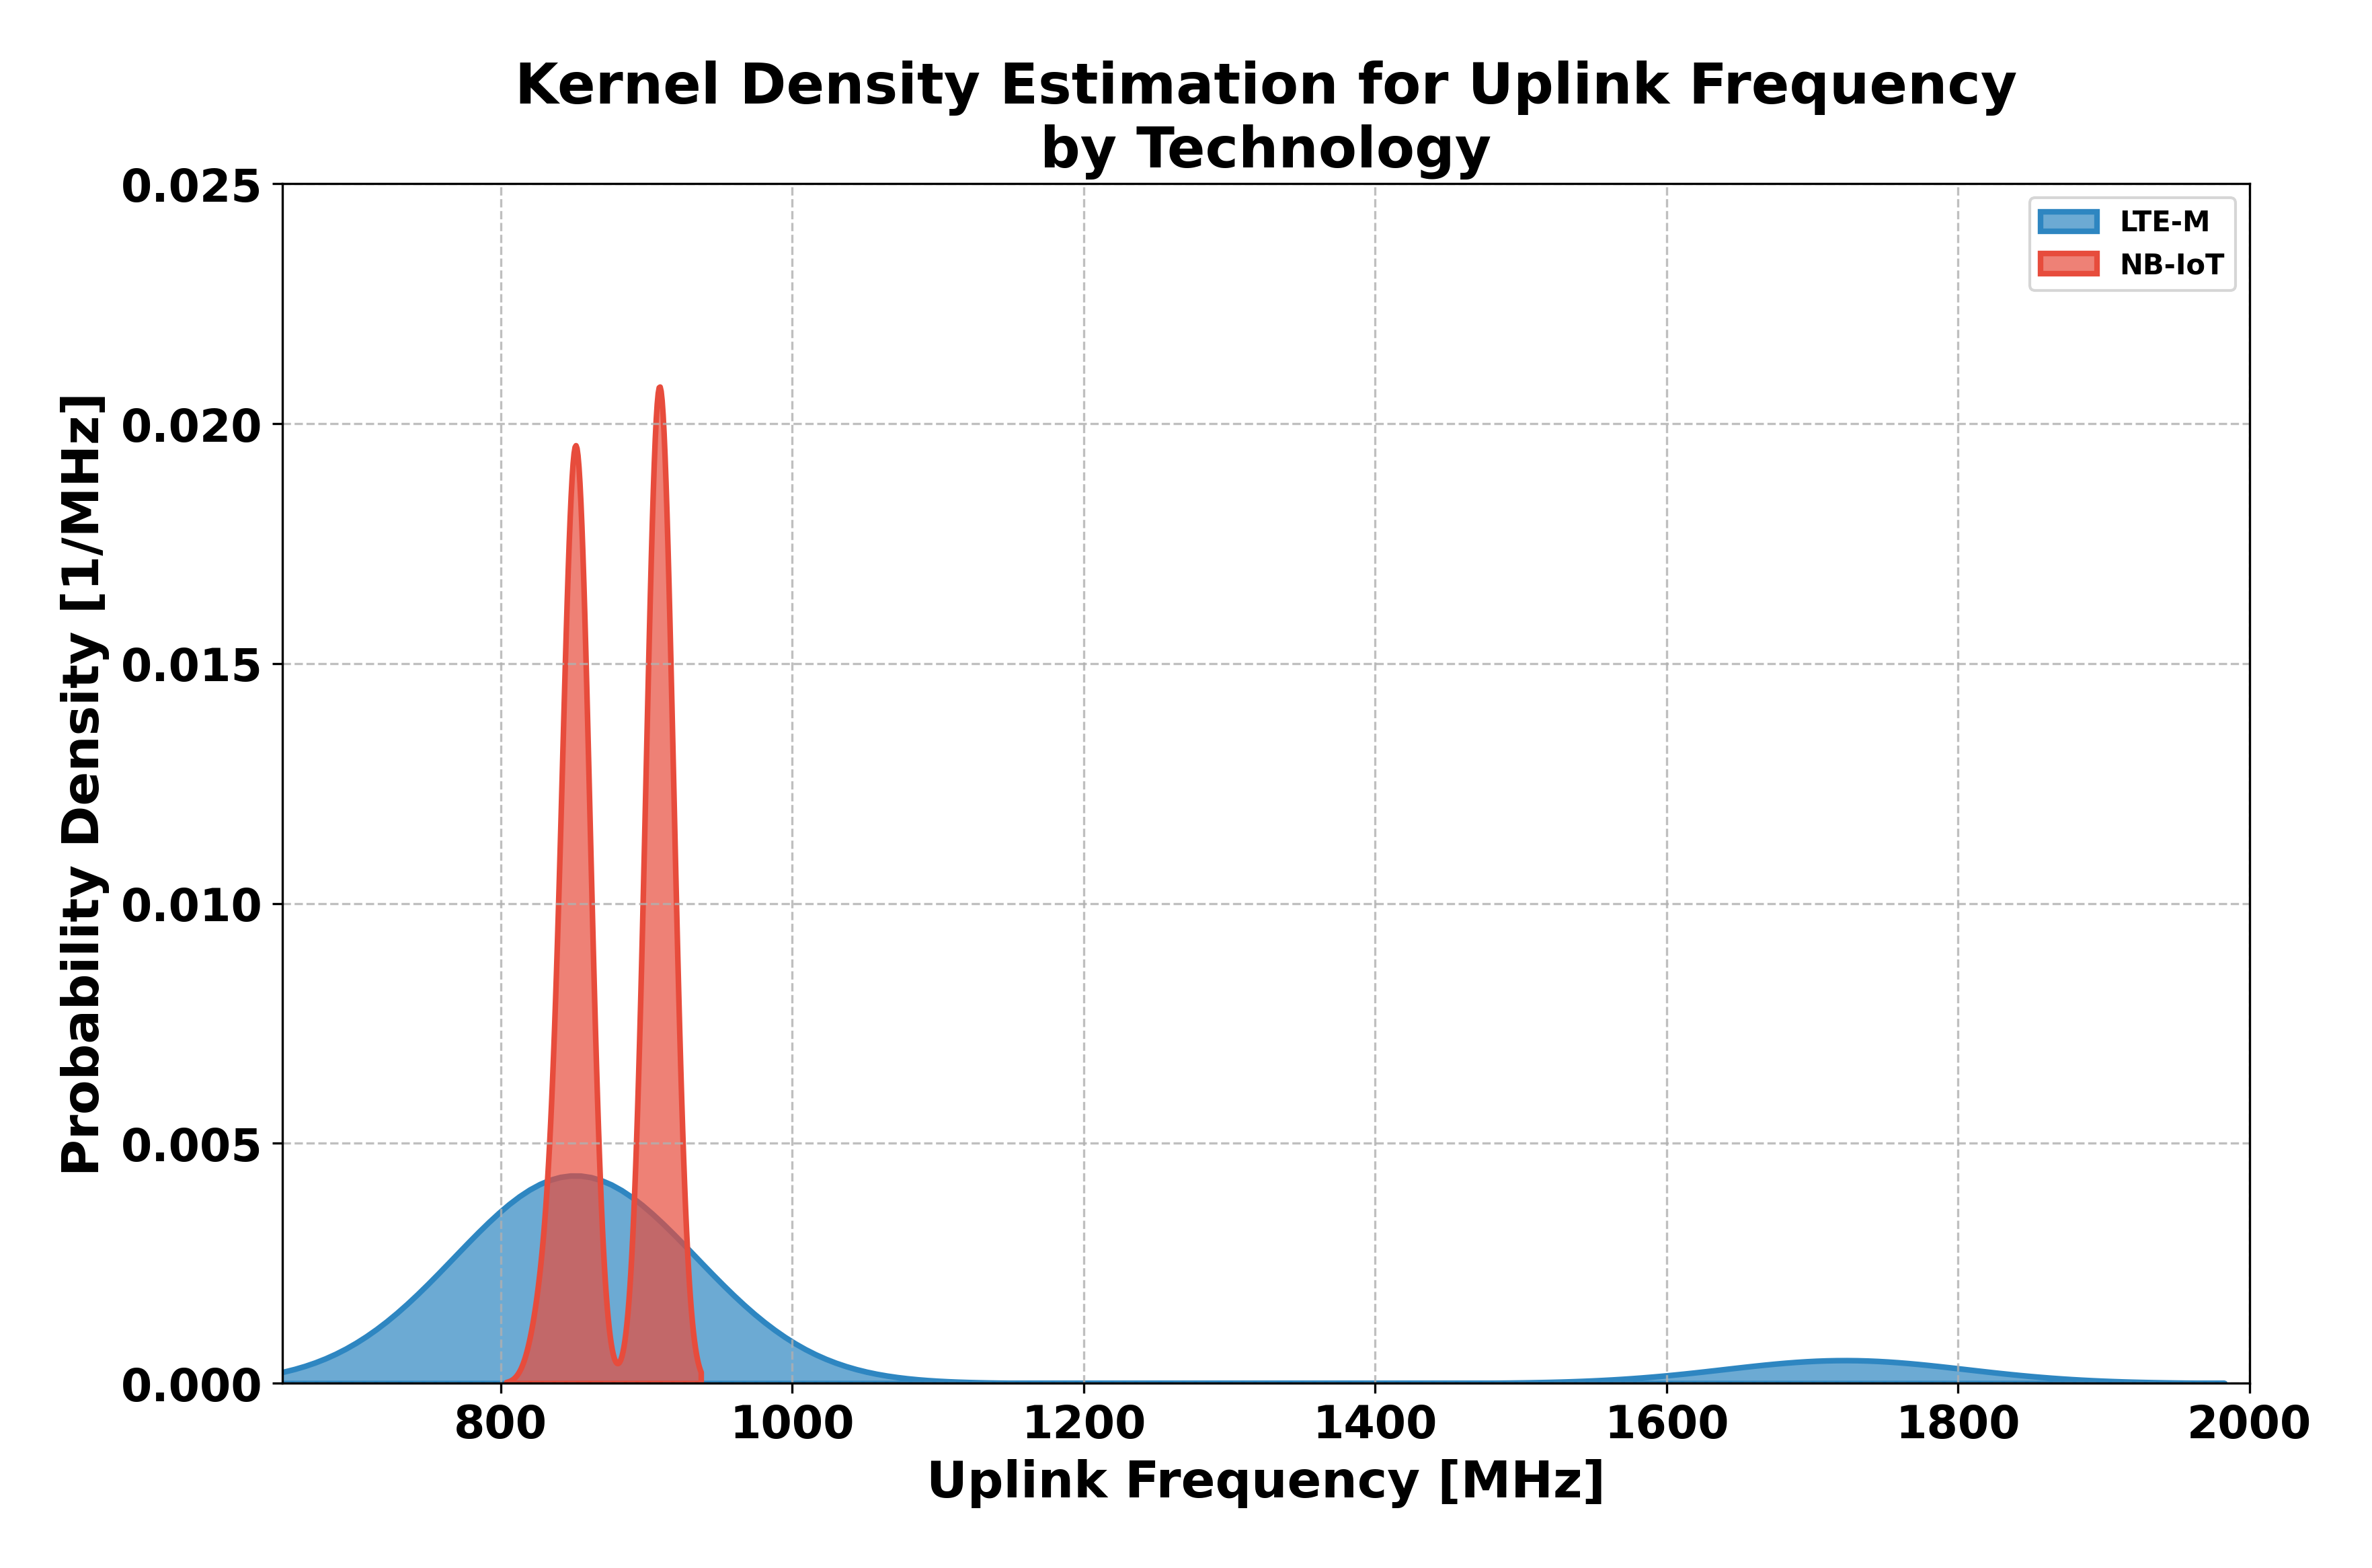
\includegraphics[width=1.0\textwidth]{uplink_frequency_frequency_kde.png}
    \caption{\textbf{Uplink Frequency Distribution} \\ The figure shows the uplink frequencies used for \gls{nbiot} and \gls{ltem} connections. Frequencies are derived from EARFCN values and reflect the radio access technology used.}
    \label{fig:uplink_frequency}
\end{figure}

\FloatBarrier
\subsubsection*{Downlink Frequency Analysis} \label{sec:downlink_frequency_analysis}
The downlink frequency analysis, shown in Figure \ref{fig:downlink_frequency}, reveals that \gls{ltem} operates on Band 20 (791-821 MHz) and Band 3 (1805-1880 MHz) for downlink transmission. \gls{nbiot} utilizes Band 8 (925-960 MHz) and Band 20 (791-821 MHz) for downlink. Similar to uplink patterns, \gls{nbiot} exhibits lower variance in downlink frequency usage compared to \gls{ltem}, with both technologies sharing the lower frequency Band 20 while using different additional bands.

% Figure: Downlink Frequency
\begin{figure}[htbp]
    \centering
    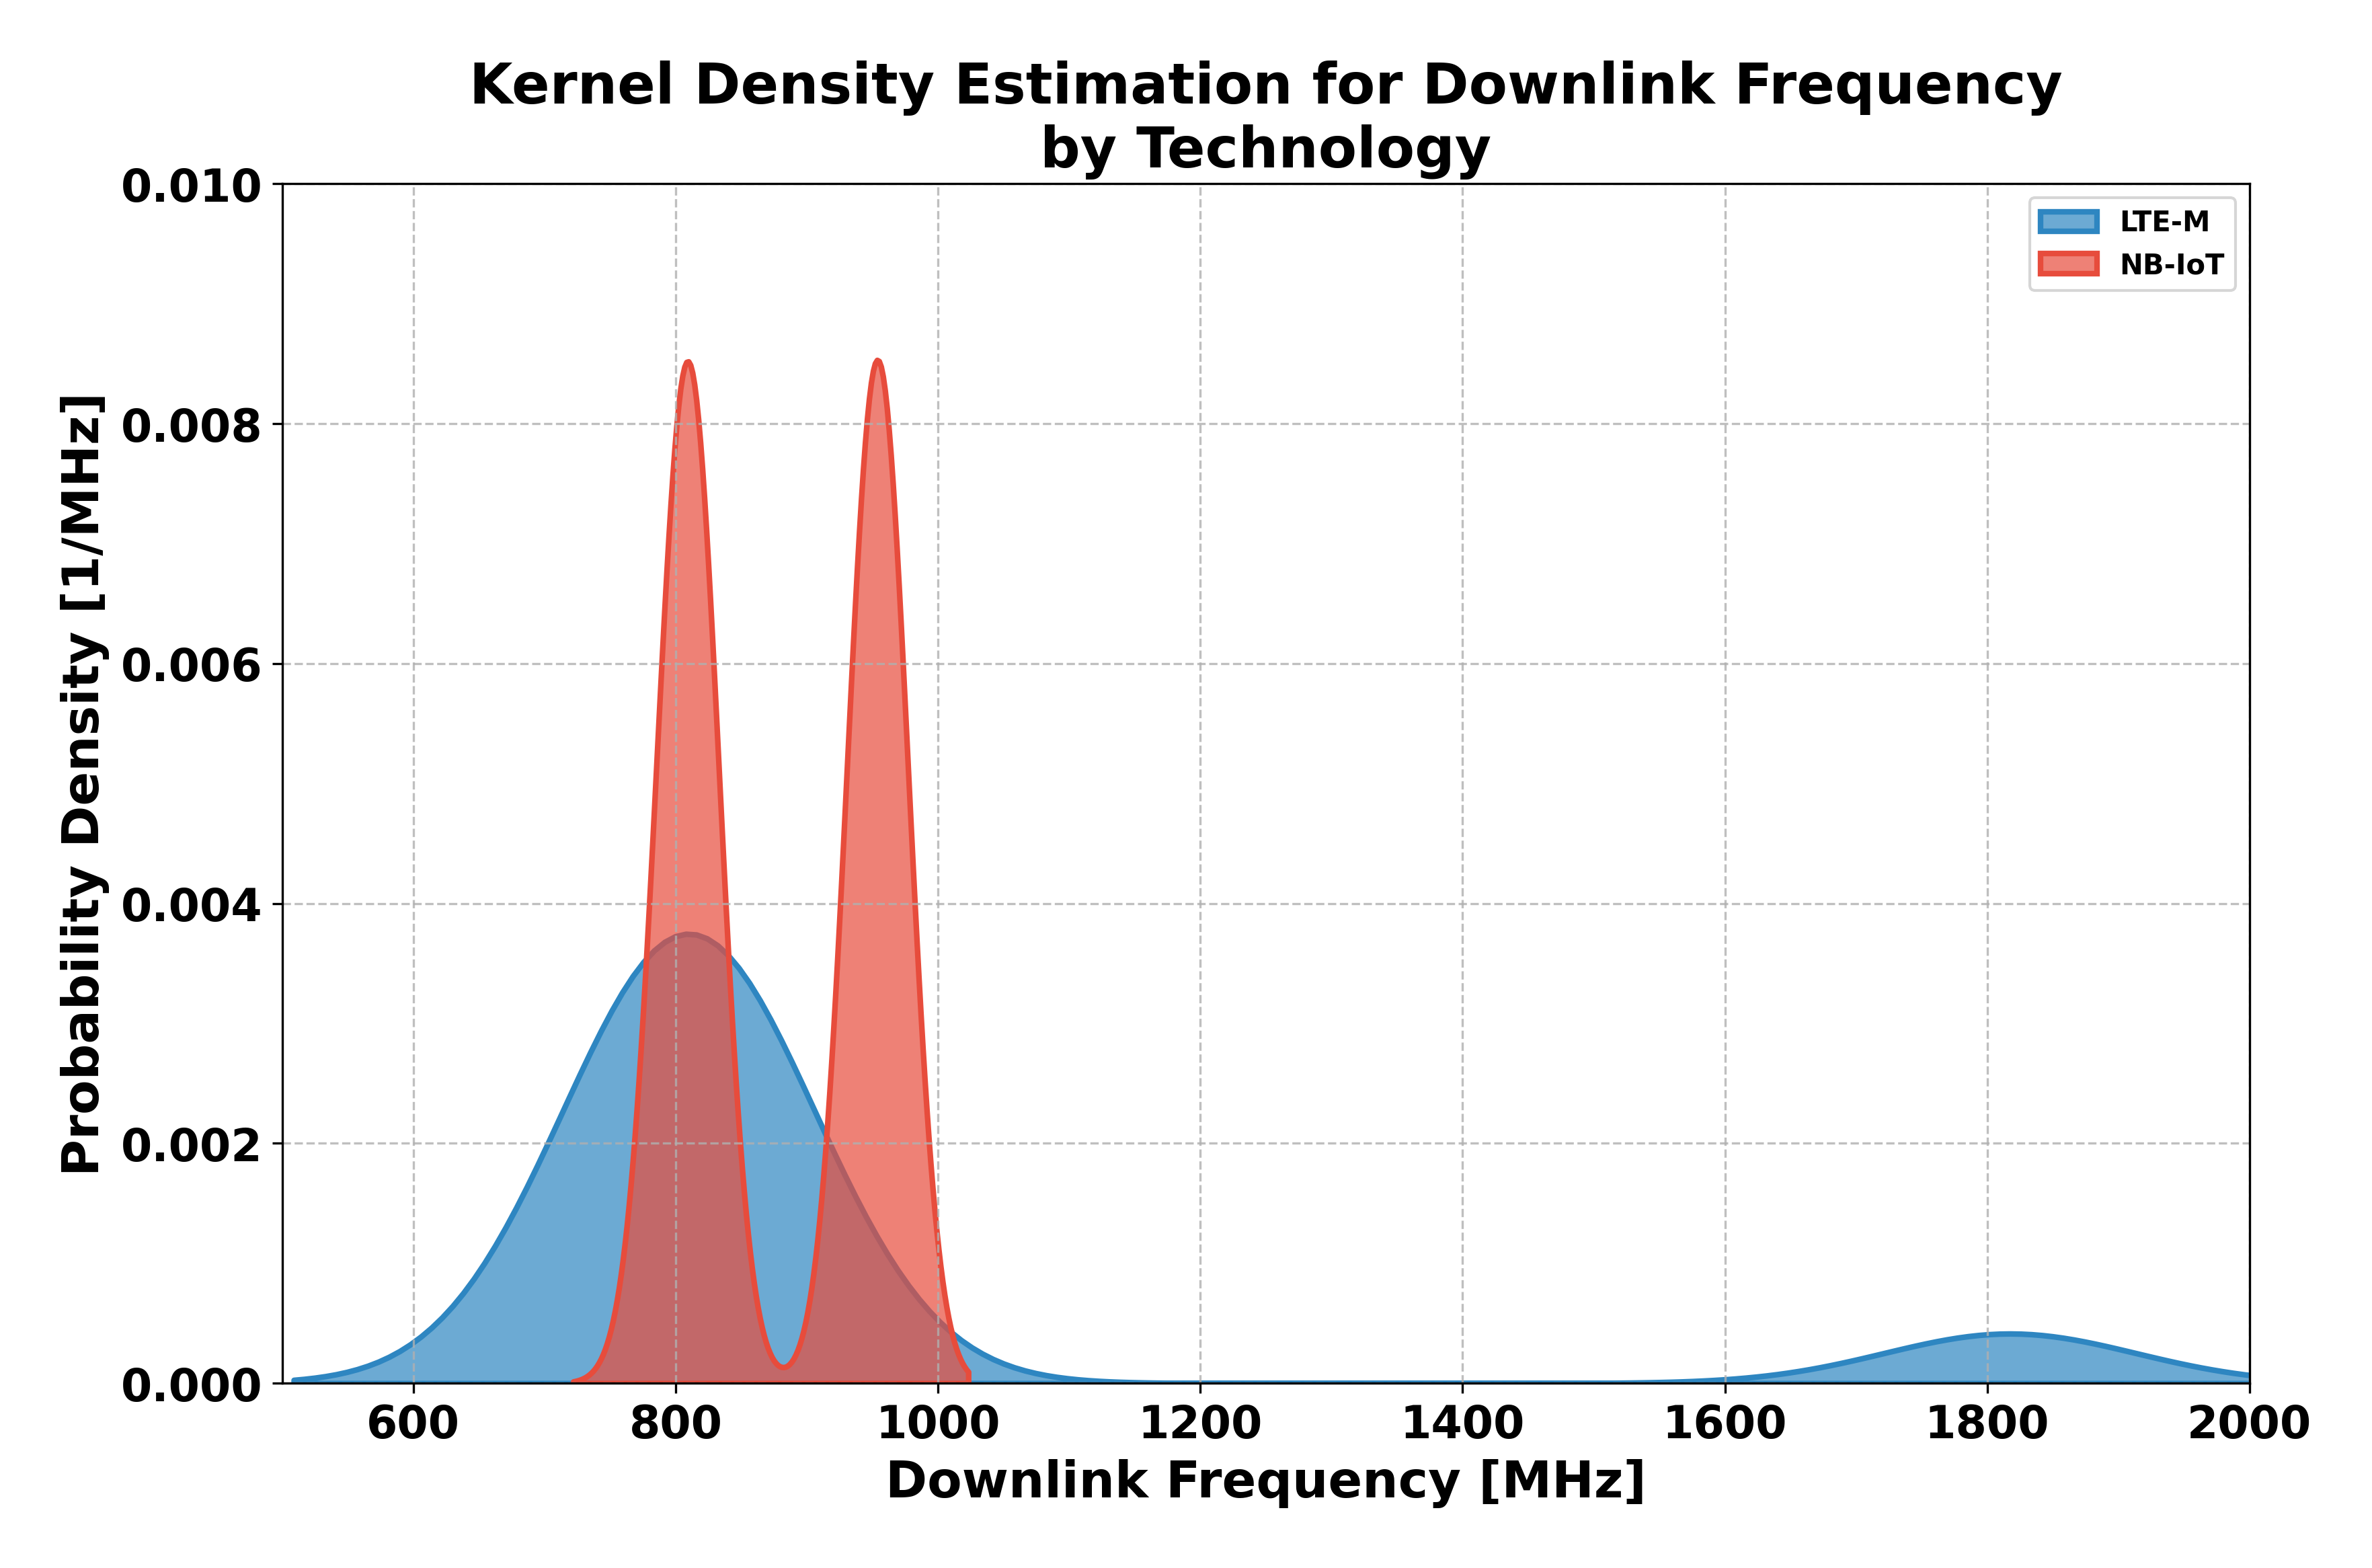
\includegraphics[width=1.0\textwidth]{downlink_frequency_frequency_kde.png}
    \caption{\textbf{Downlink Frequency Distribution} \\ The figure shows the downlink frequencies used for \gls{nbiot} and \gls{ltem} connections. Frequencies are derived from EARFCN values and reflect the radio access technology used.}
    \label{fig:downlink_frequency}
\end{figure}
\FloatBarrier
\subsubsection*{Technology Radar Comparison} \label{sec:technology_radar_comparison}

Figure \ref{fig:technology_radar} provides a multi-dimensional radar chart comparison of \gls{nbiot} and \gls{ltem} performance across normalized metrics. The visualization enables simultaneous assessment of multiple performance indicators, with values normalized to ensure cross-metric comparability and outlier suppression. The radar chart reveals that while some metrics such as transmit repetitions and downlink pathloss show relatively similar performance between technologies, others including throughput, connection time, \gls{rsrq}, \gls{snr}, and \gls{rsrp} demonstrate substantial differences.

% Figure: Technology Radar Comparison
\begin{figure}[htbp]
    \centering
    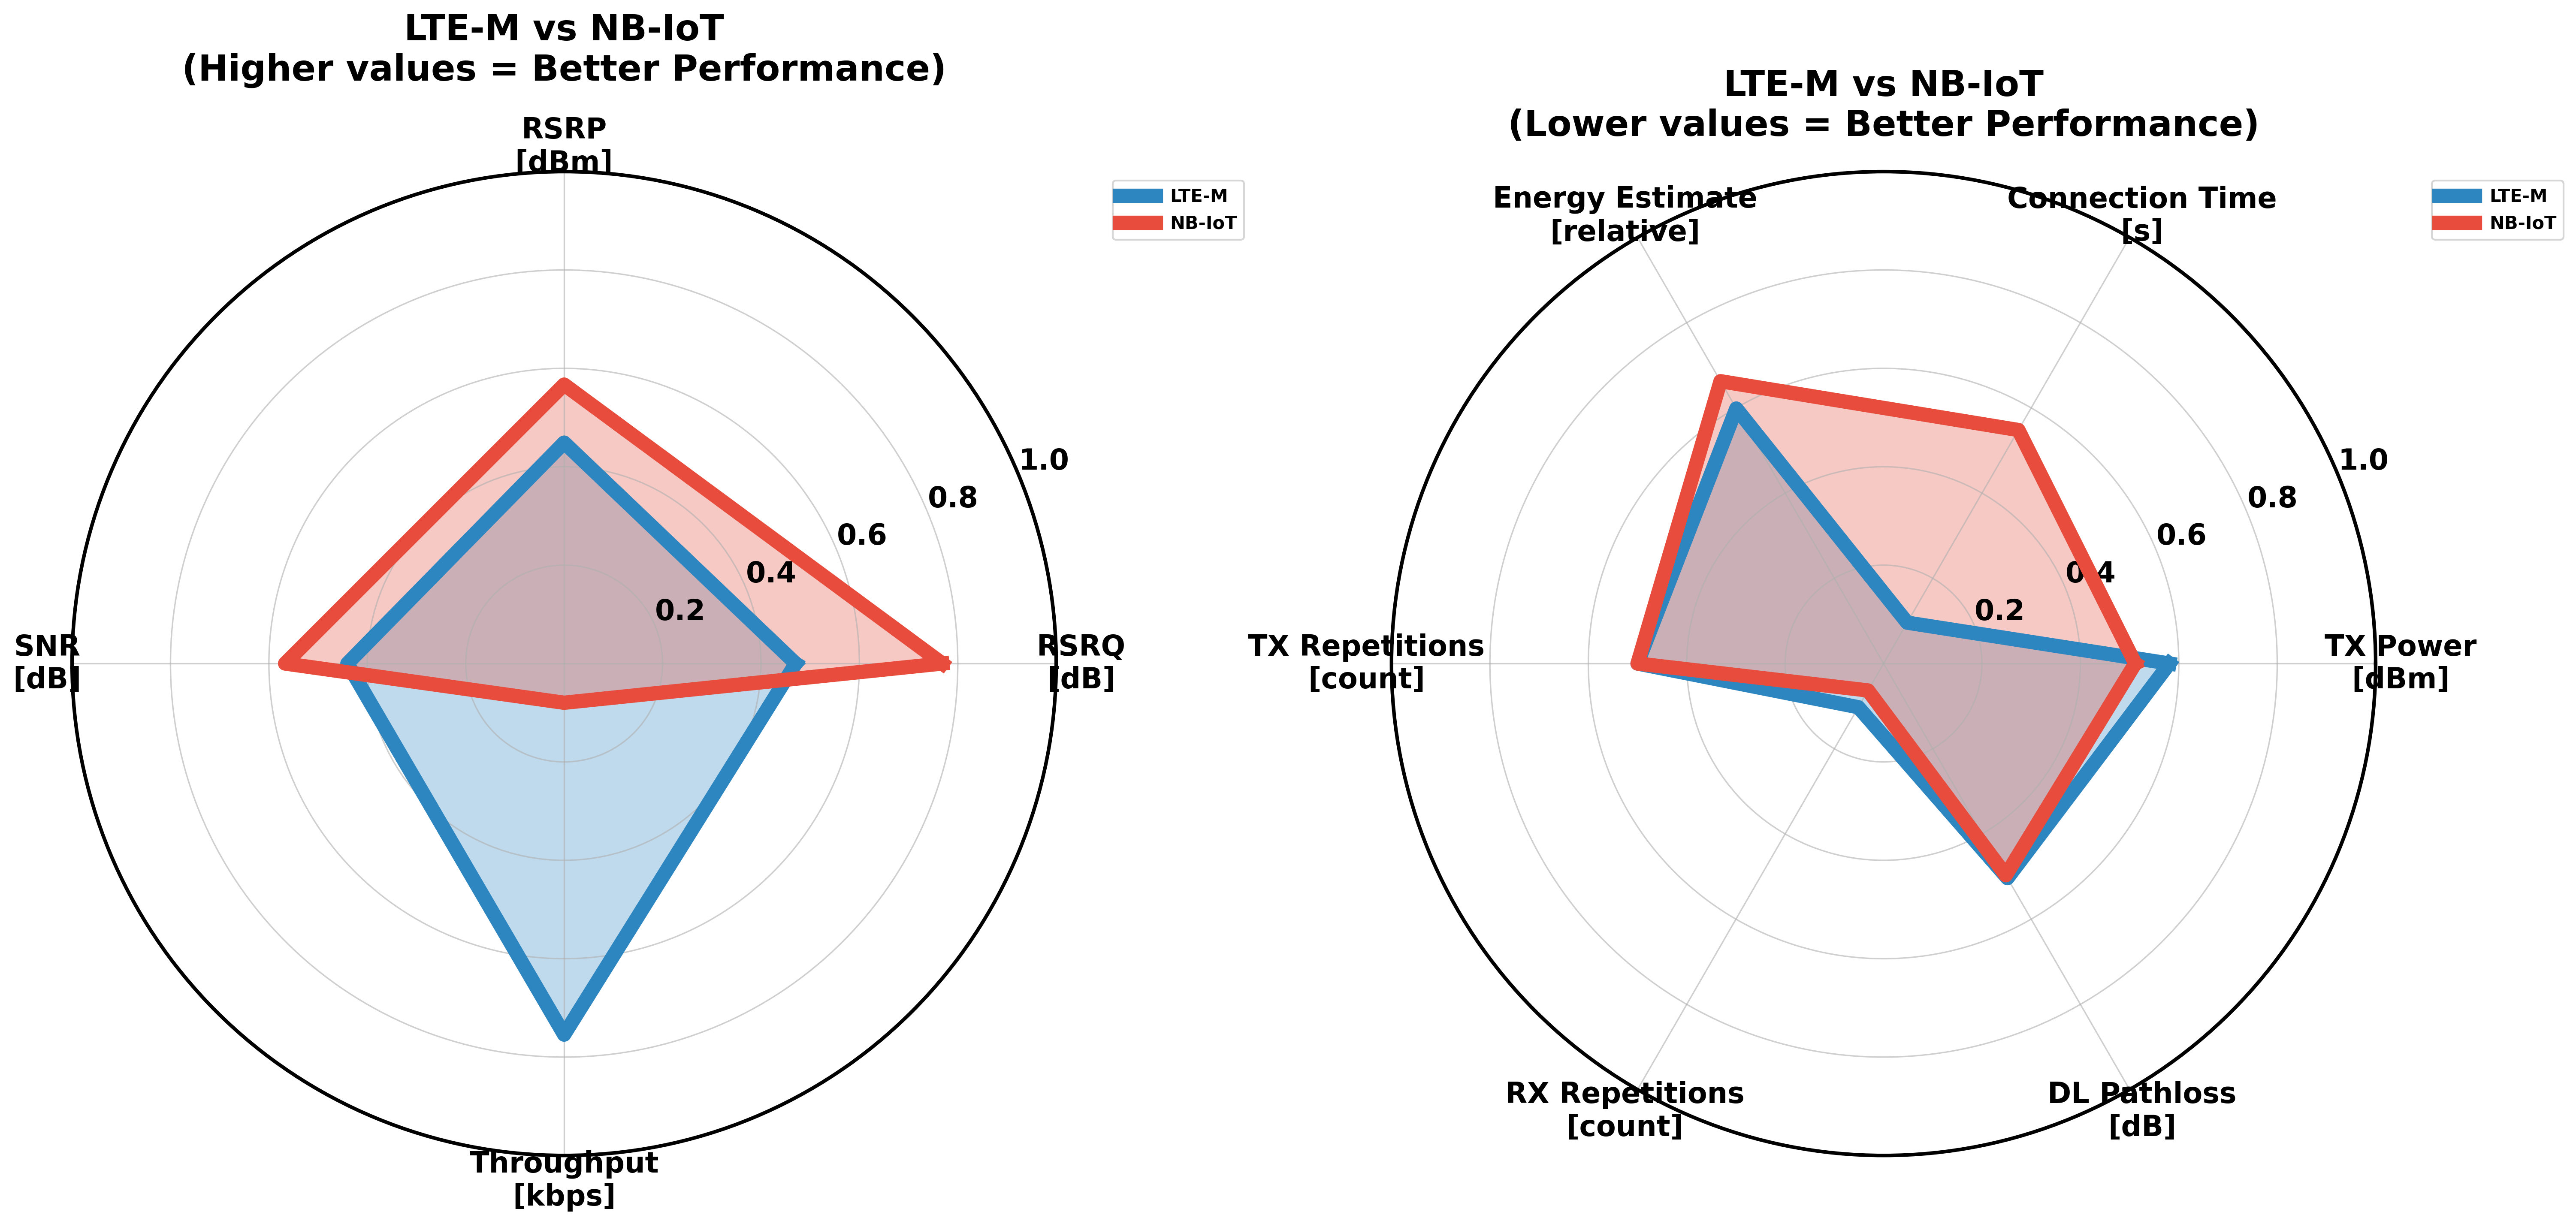
\includegraphics[width=1.0\textwidth]{technology_radar_comparison.png}
    \caption{\textbf{Technology Comparison Radar Chart} \\ The figure provides a multi-dimensional comparison of \gls{nbiot} and \gls{ltem} across various performance metrics. The left radar chart shows metrics where higher values indicate better performance, while the right radar chart shows metrics where lower values indicate better performance.}
    \label{fig:technology_radar}
\end{figure}

Figure \ref{fig:communication_technology_comparison_summary} presents a categorical performance summary highlighting the relative strengths of each technology across key performance indicators. The visualization identifies areas where \gls{nbiot} demonstrates superior performance (including transmit power efficiency, \gls{rsrp}, \gls{rsrq}, and \gls{snr}) versus areas where \gls{ltem} dominates (including connection time, throughput, and transmission repetitions).

% Figure: Communication Technology Comparison Summary
\begin{figure}[htbp]
    \centering
    \includegraphics[width=1.0\textwidth]{communication_technology_comparison.png}
    \caption{\textbf{Communication Technology Comparison Summary} \\ The figure summarizes the  performance differences between \gls{nbiot} and \gls{ltem} across key metrics. It highlights the strengths and weaknesses of each technology in terms of signal quality, connection time, and energy efficiency.}
    \label{fig:communication_technology_comparison_summary}
\end{figure}

The communication technology comparison reveals performance characteristics for each technology. \gls{nbiot} demonstrates superior signal quality metrics (\gls{rsrp}, \gls{rsrq}, \gls{snr}) and energy efficiency, while \gls{ltem} provides faster connection establishment and significantly higher data throughput capabilities. These findings build the foundation for protocol-specific performance analysis in the following subsection.

\FloatBarrier
\subsection{Protocol and Technology Combination Analysis} \label{sec:results_by_protocol_technology}

This subsection shows the performance characteristics of \gls{mqtt} and \gls{lwm2m} protocols operating across both \gls{nbiot} and \gls{ltem} technologies, resulting in four protocol-technology combinations. The analysis focuses on connection establishment, security handshake procedures, end-to-end latency, and network behavior metrics.

\subsubsection*{Connection Time Distribution}

Figure \ref{fig:connection_time_all} presents the full connection time analysis across all four protocol-technology combinations. The upper plot shows the kernel density estimation revealing the distribution characteristics, while the lower plot provides confidence interval comparison of mean values. The results show that \gls{mqtt} over \gls{ltem} achieves the fastest connection establishment with a mean time of 2.771 seconds, while \gls{mqtt} over \gls{nbiot} requires the longest connection time with a mean of 6.518 seconds. The Kruskal-Wallis test shows a p-value of p < 0.001, providing highly significant evidence of connection time differences across the combinations. The \gls{kde} visualization reveals that \gls{mqtt} over \gls{nbiot} and \gls{lwm2m} over \gls{ltem} exhibit substantially higher variance in connection times compared to the other combinations, which is confirmed by the confidence interval analysis showing broader uncertainty ranges for these combinations.

% Figure: Connection Time Combined
\begin{figure}[htbp]
    \centering
    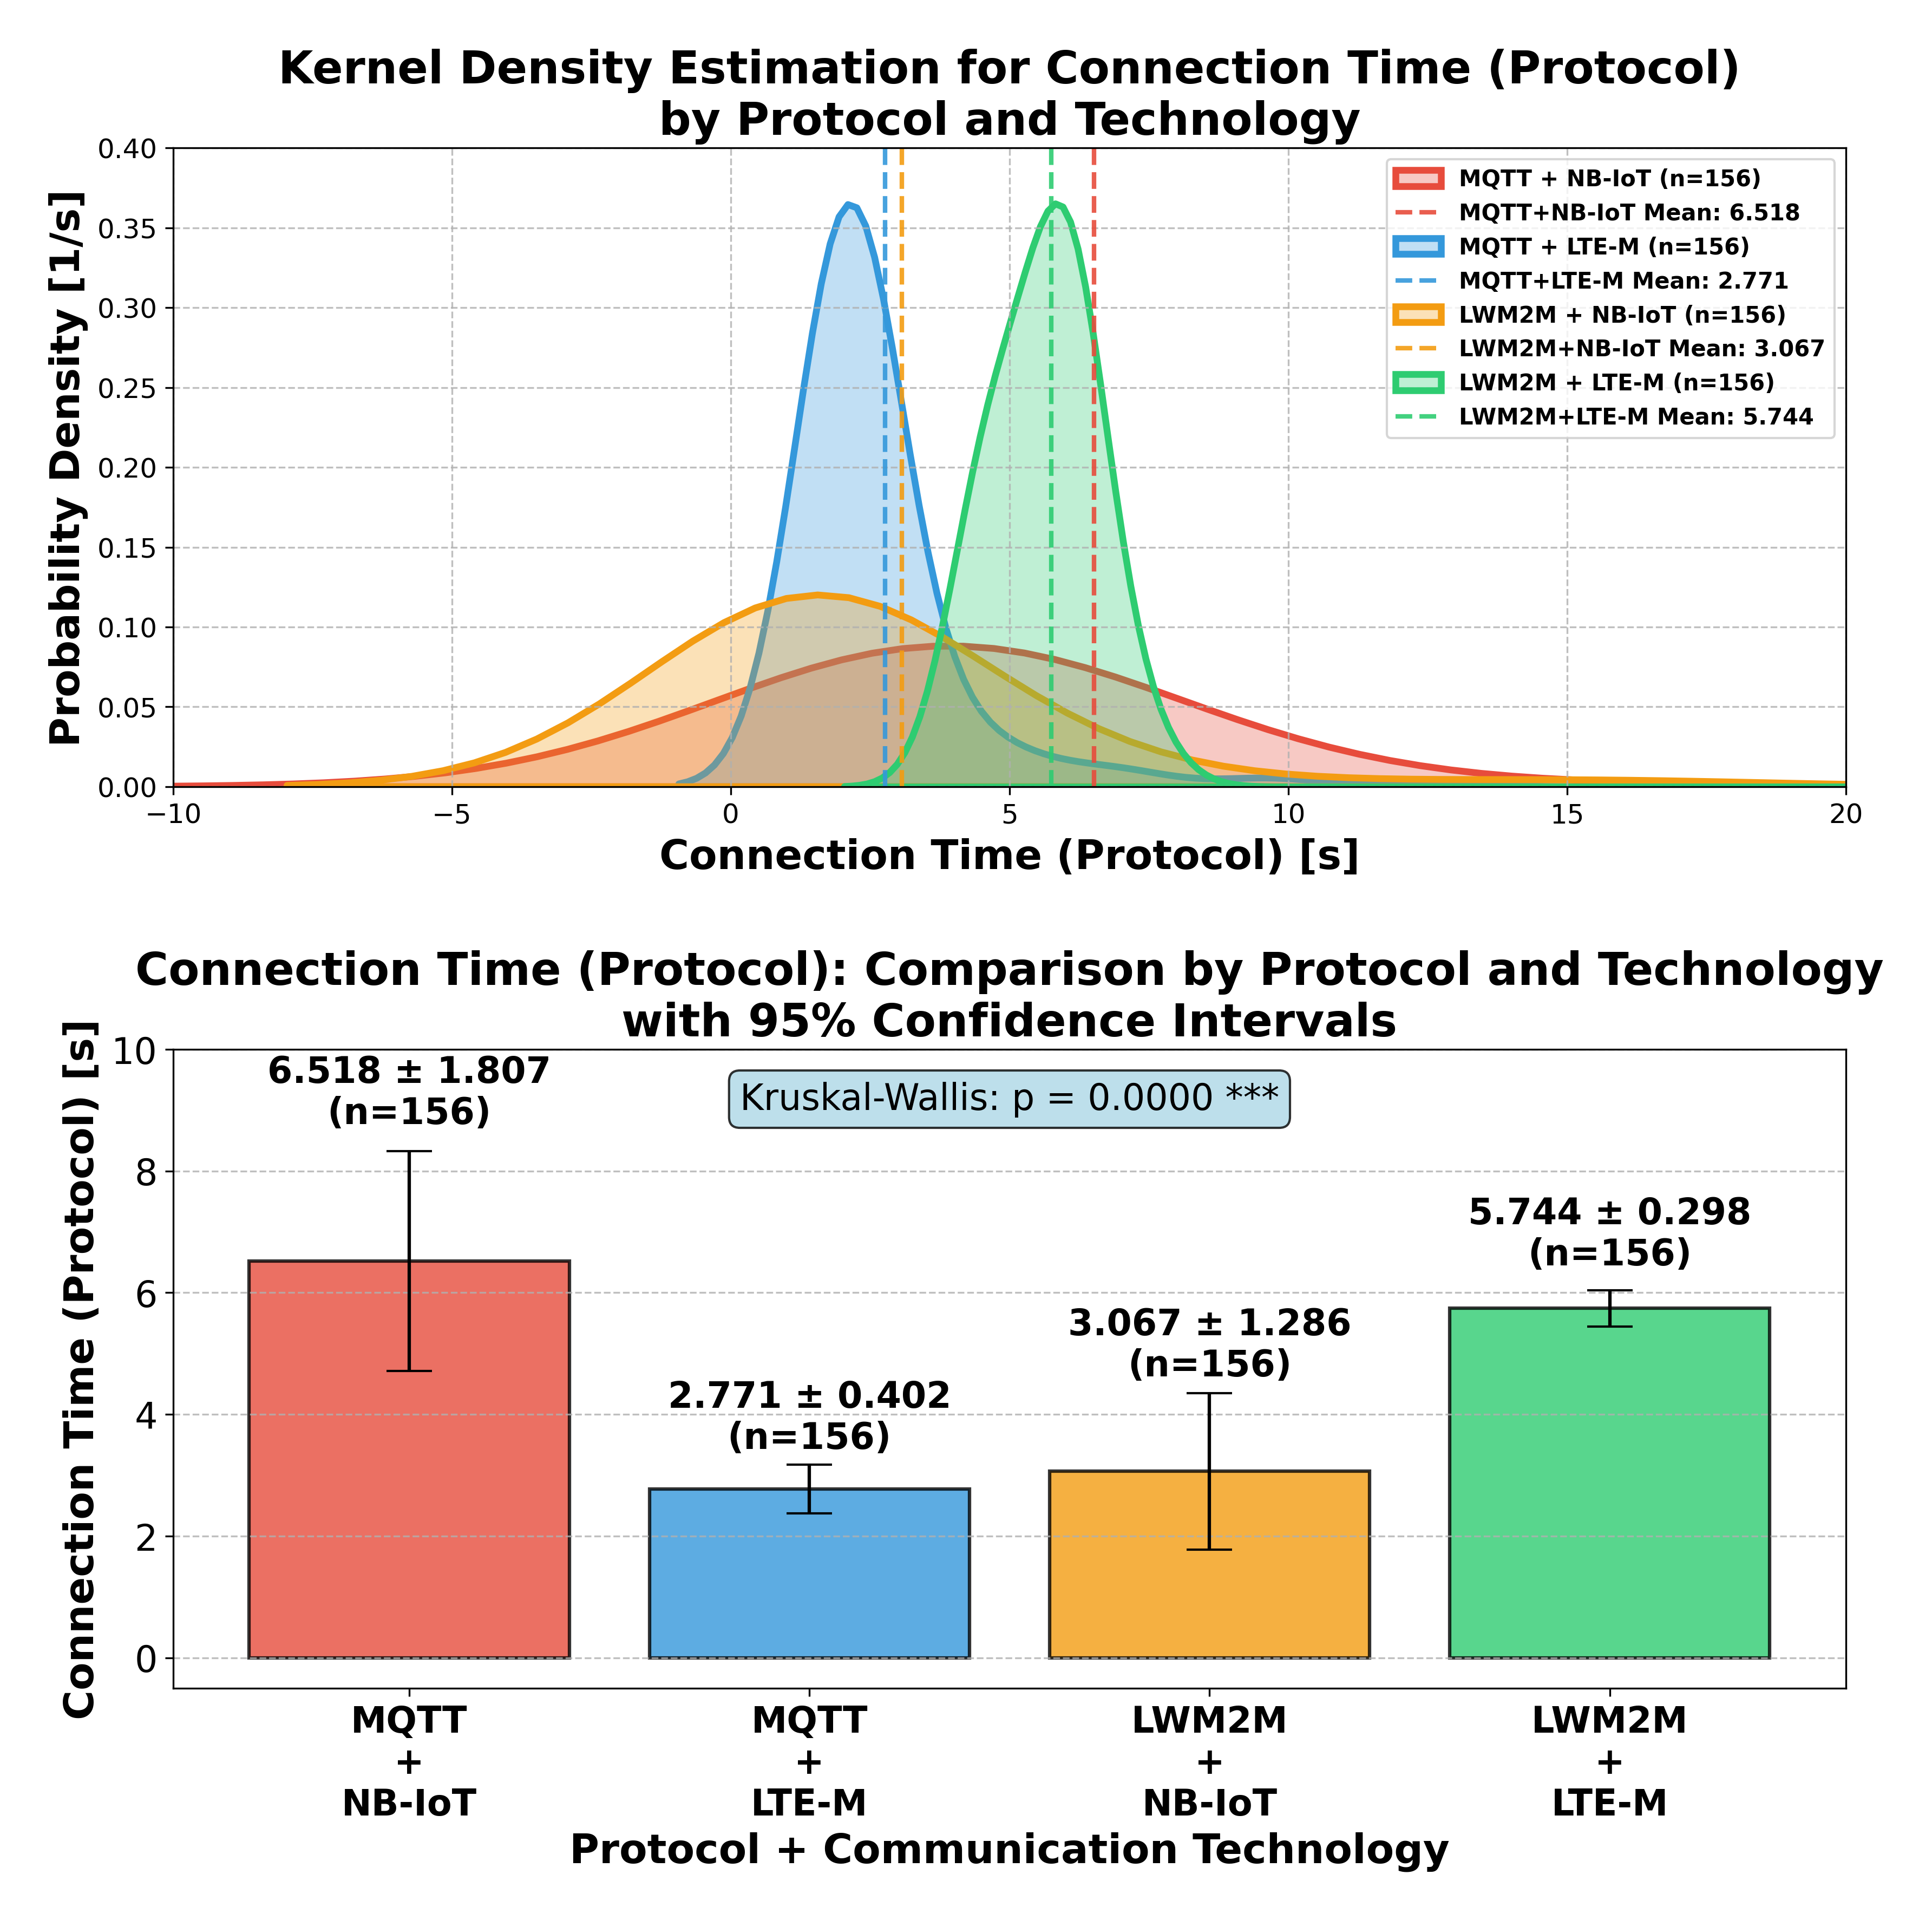
\includegraphics[width=1.0\textwidth]{connection_time_all_protocol_tech_kde_ci.png}
    \caption{\textbf{Connection Time Distribution and Comparison} \\ The figure shows protocol connection time distributions (top) and confidence interval comparison (bottom) across protocol and technology combinations: \gls{mqtt}+\gls{nbiot}, \gls{mqtt}+\gls{ltem}, \gls{lwm2m}+\gls{nbiot}, and \gls{lwm2m}+\gls{ltem}.}
    \label{fig:connection_time_all}
\end{figure}
\FloatBarrier
\subsubsection*{Security Handshake Time Distribution} \label{sec:handshake_time_analysis}

The security handshake time analysis, illustrated in Figure \ref{fig:handshake_time_all}, reveals significant performance variations across protocol-technology combinations through both distribution analysis and statistical comparison. The KDE plot demonstrates that \gls{lwm2m} over \gls{nbiot} achieves the fastest security establishment with a mean handshake time of 1.021 seconds, while \gls{mqtt} over \gls{nbiot} requires the longest handshake time at 7.008 seconds. The distribution analysis shows \gls{mqtt} over \gls{nbiot} demonstrating the highest variance in handshake times, whereas \gls{lwm2m} over \gls{nbiot} shows the most consistent performance. The confidence interval comparison confirms these findings, with statistical analysis using the Kruskal-Wallis test providing highly significant differences (p < 0.001) in security handshake times across all combinations.

% Figure: Handshake Time Combined
\begin{figure}[htbp]
    \centering
    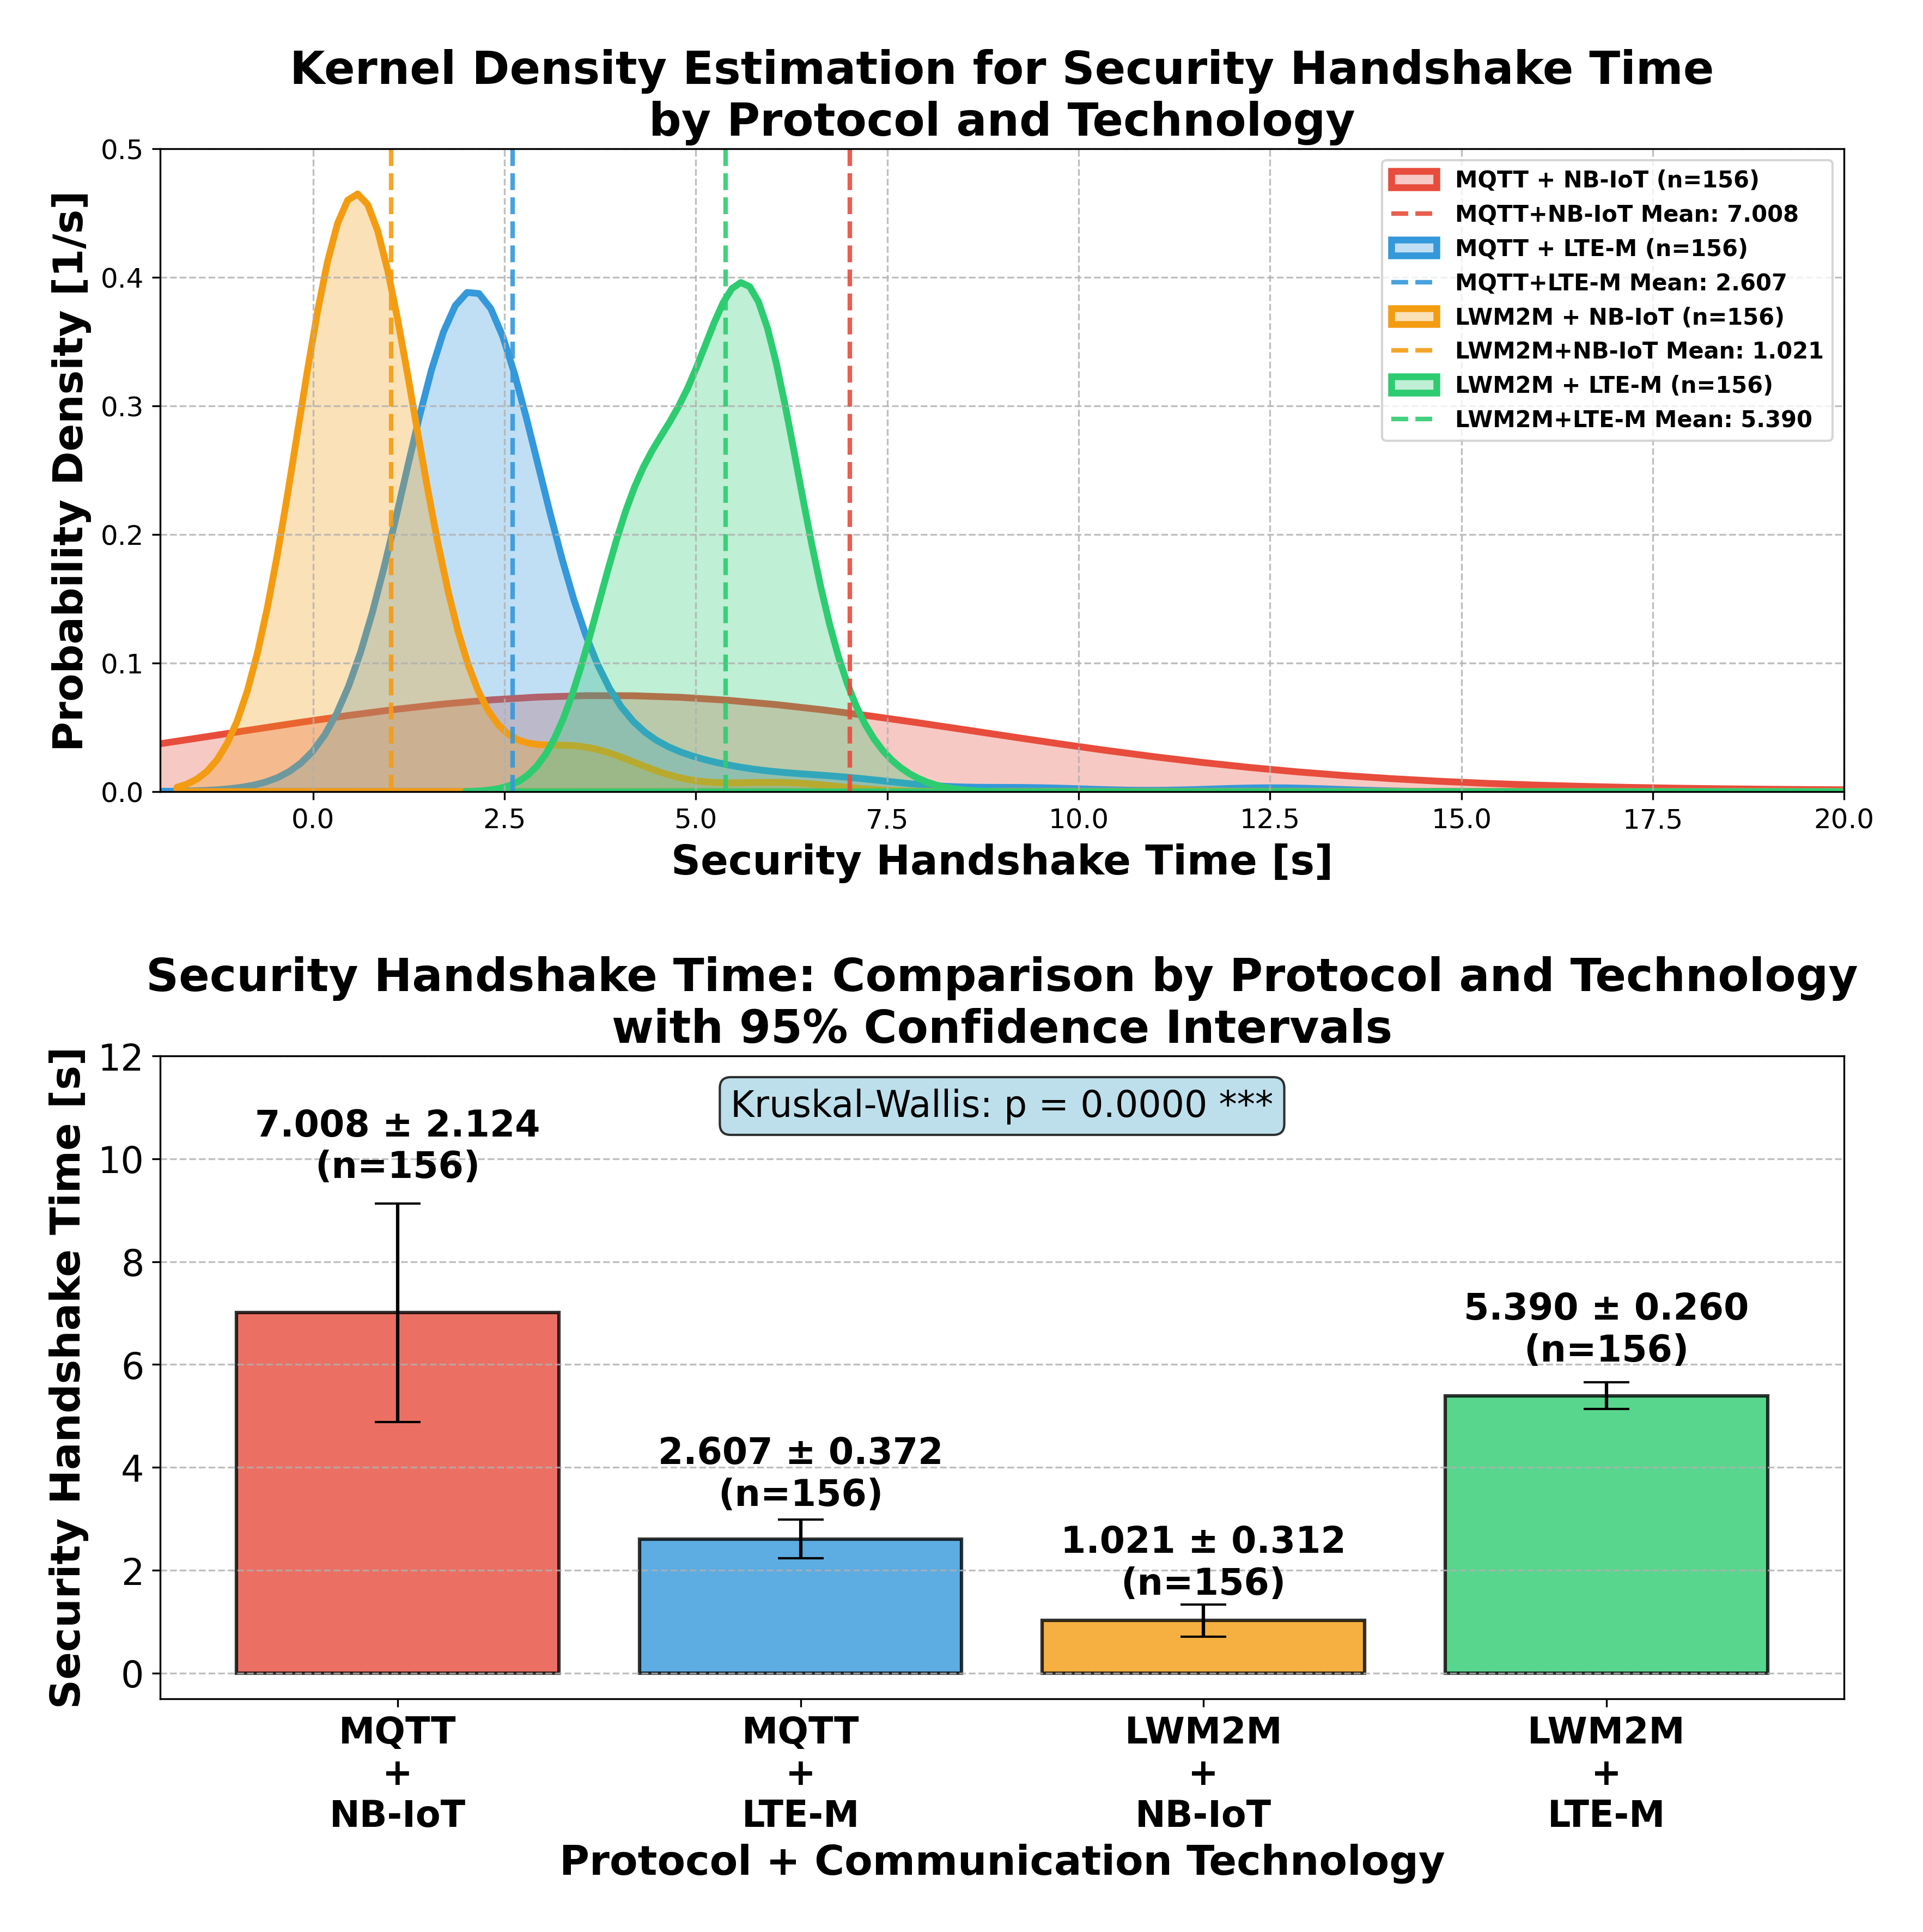
\includegraphics[width=1.0\textwidth]{handshake_time_all_protocol_tech_kde_ci.png}
    \caption{\textbf{Security Handshake Time Distribution and Comparison} \\ The figure shows the distribution (top) and confidence interval comparison (bottom) of time required for security handshake establishment across \gls{mqtt} and \gls{lwm2m} protocols on both \gls{nbiot} and \gls{ltem} technologies.}
    \label{fig:handshake_time_all}
\end{figure}
\FloatBarrier
\subsubsection*{Latency Distribution} \label{sec:latency_analysis}

Figure \ref{fig:latency_all} presents the latency analysis across all protocol-technology combinations, combining distribution visualization with statistical comparison. The kernel density estimation shows that \gls{mqtt} over \gls{ltem} achieves the lowest latency with a mean of 0.134 seconds, while \gls{lwm2m} over \gls{nbiot} shows substantially higher latency with a mean of 1.402 seconds. The distribution analysis reveals that \gls{lwm2m} over \gls{nbiot} demonstrates considerably higher variance compared to other combinations, while \gls{mqtt} over \gls{ltem} shows the most consistent latency performance. The confidence interval comparison confirms these observations, with the Kruskal-Wallis test providing highly significant differences (p < 0.001) in latency performance across combinations.

% Figure: Latency Combined
\begin{figure}[htbp]
    \centering
    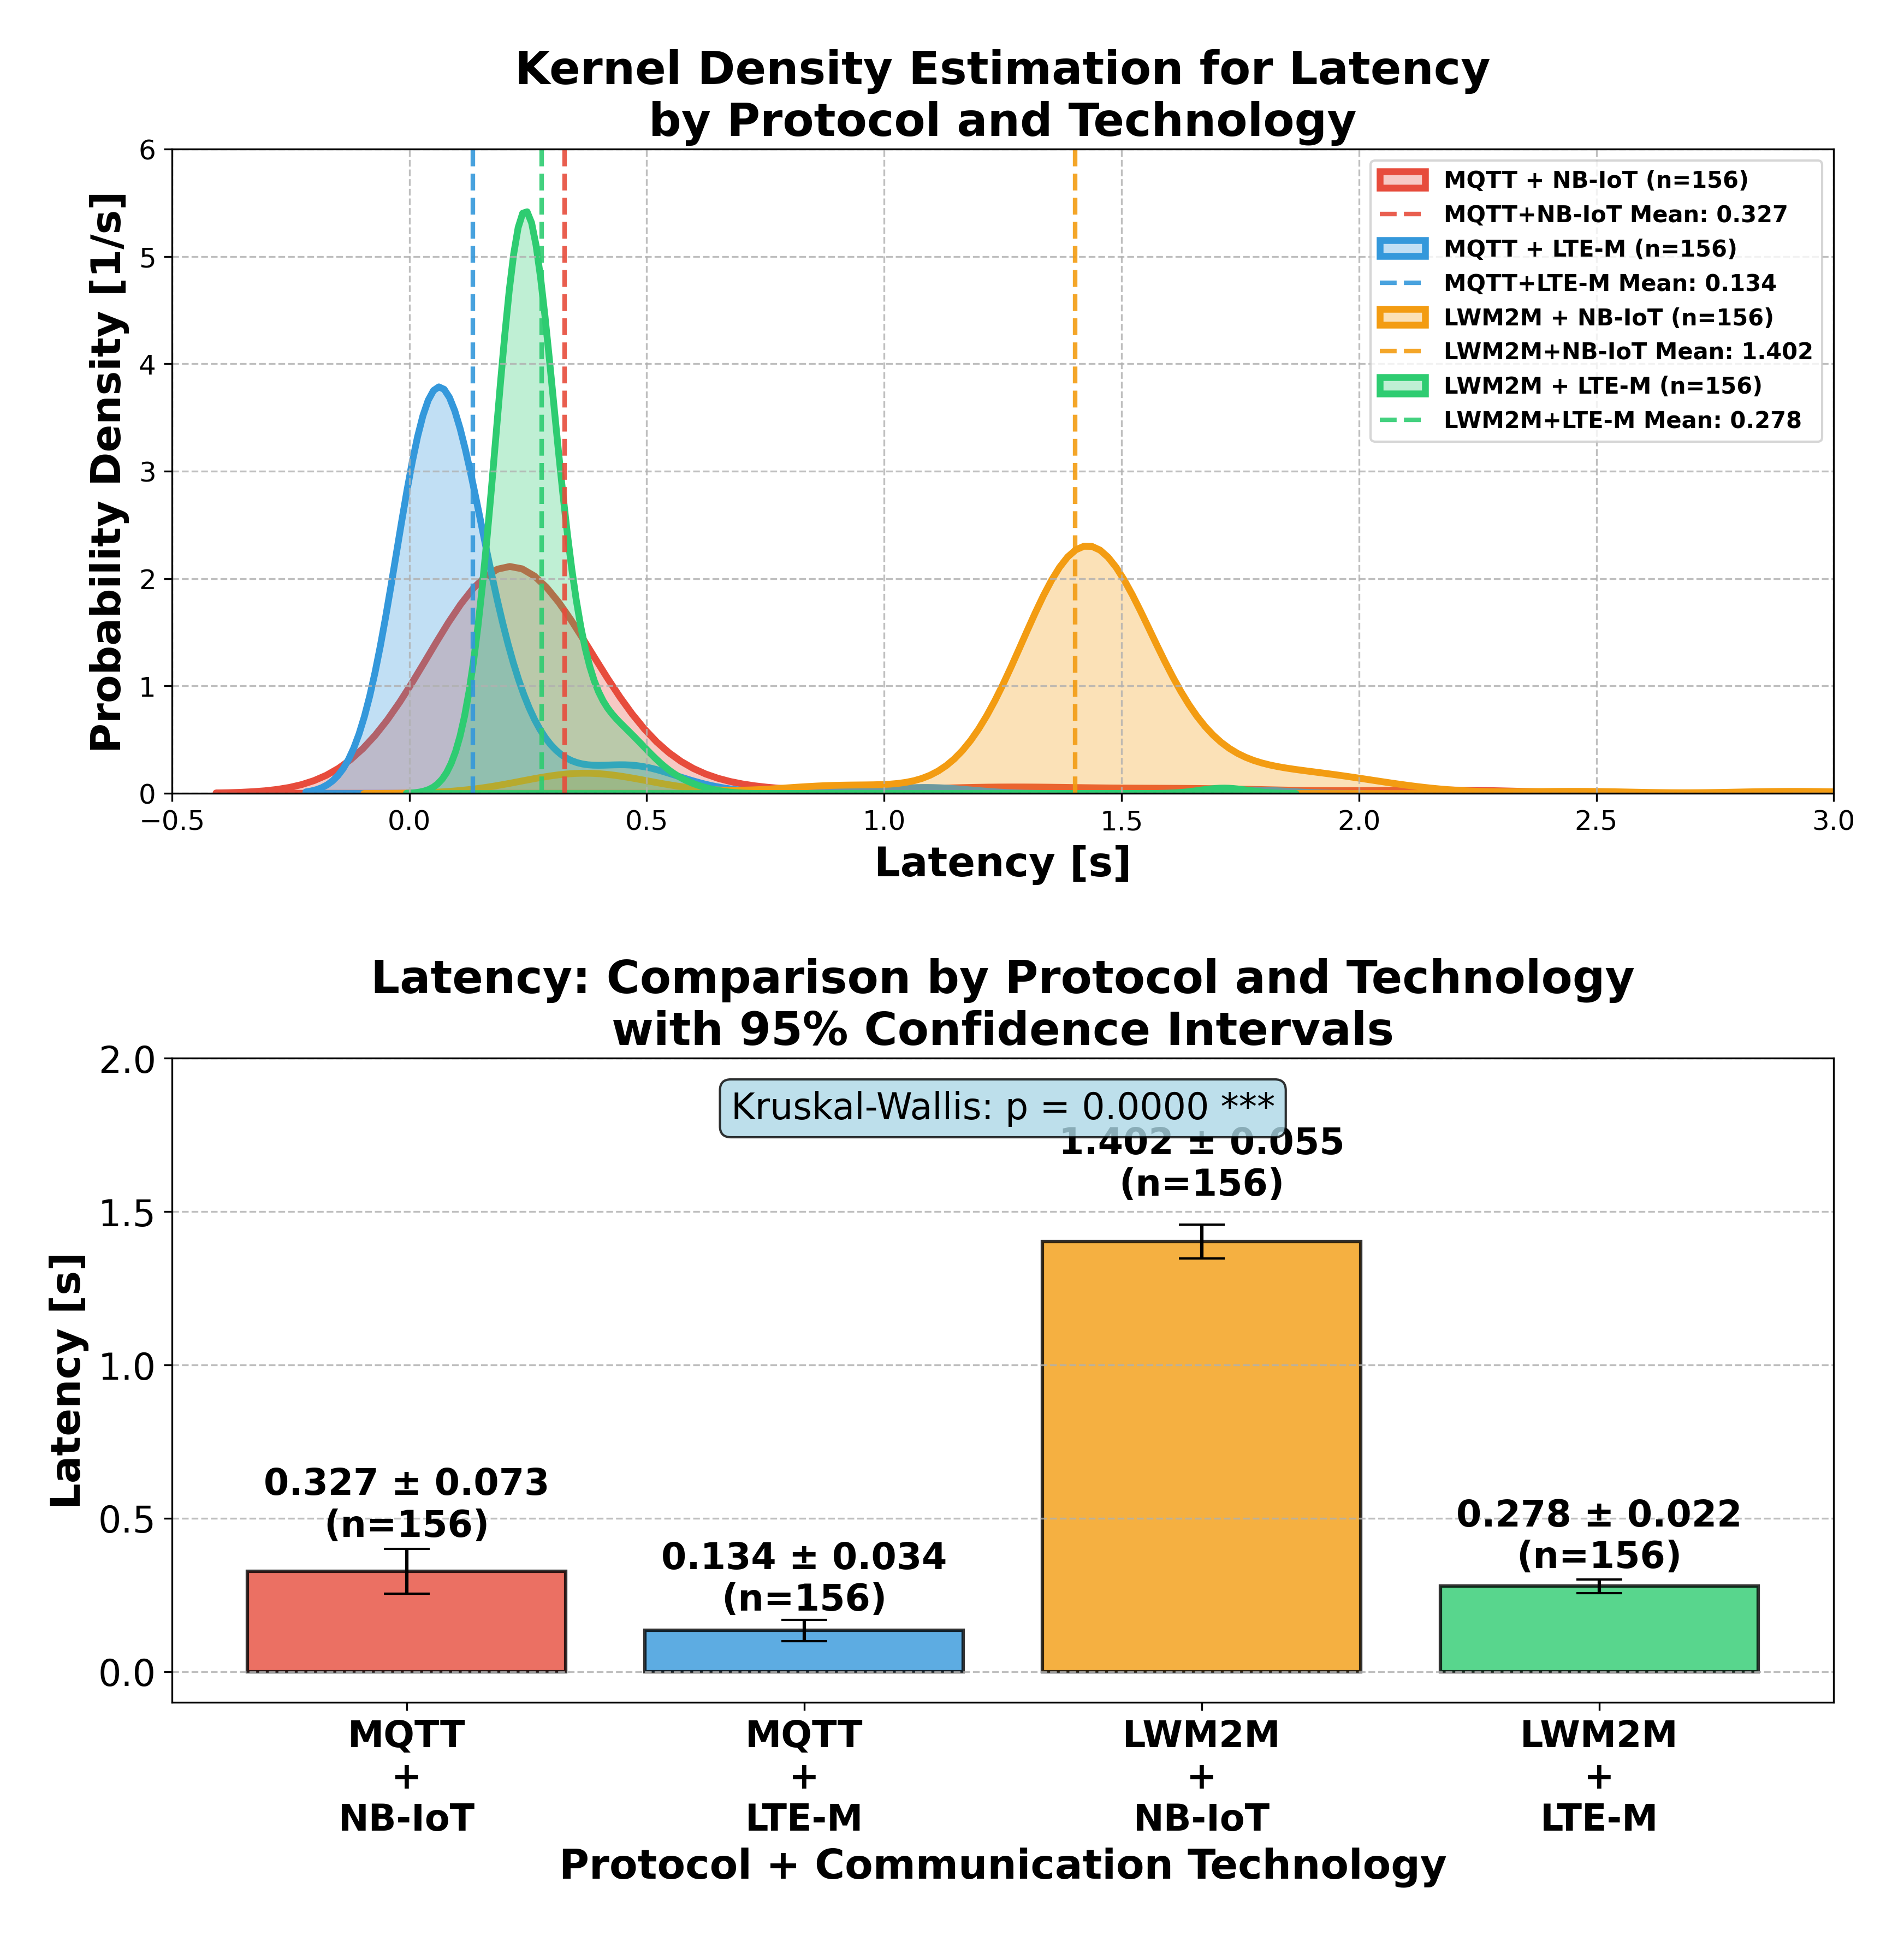
\includegraphics[width=1.0\textwidth]{latency_all_protocol_tech_kde_ci.png}
    \caption{\textbf{End-to-end Latency Distribution and Comparison} \\ The figure shows latency distributions (top) and confidence interval comparison (bottom) across all four protocol-technology combinations, indicating overall system responsiveness.}
    \label{fig:latency_all}
\end{figure}
\FloatBarrier
\subsubsection*{Network Registration Changes Analysis} \label{sec:network_registration_changes_analysis}

The network registration changes analysis, shown in Figure \ref{fig:network_registration_changes_all}, combines distribution analysis with statistical comparison to reveal comprehensive performance characteristics. The KDE visualization shows that \gls{mqtt} over \gls{nbiot} produces the fewest network registration changes with a mean of 7.045 occurrences, while \gls{lwm2m} over \gls{ltem} generates the highest number with a mean of 15.583 changes. The distribution analysis reveals that \gls{lwm2m} over \gls{ltem} has the highest variance in registration changes, while \gls{mqtt} over both \gls{ltem} and \gls{nbiot} demonstrate similar and relatively low variance characteristics. Statistical analysis using the Kruskal-Wallis test, displayed in the confidence interval comparison, confirms highly significant differences (p < 0.001) across combinations.

% Figure: Network Registration Changes Combined
\begin{figure}[htbp]
    \centering
    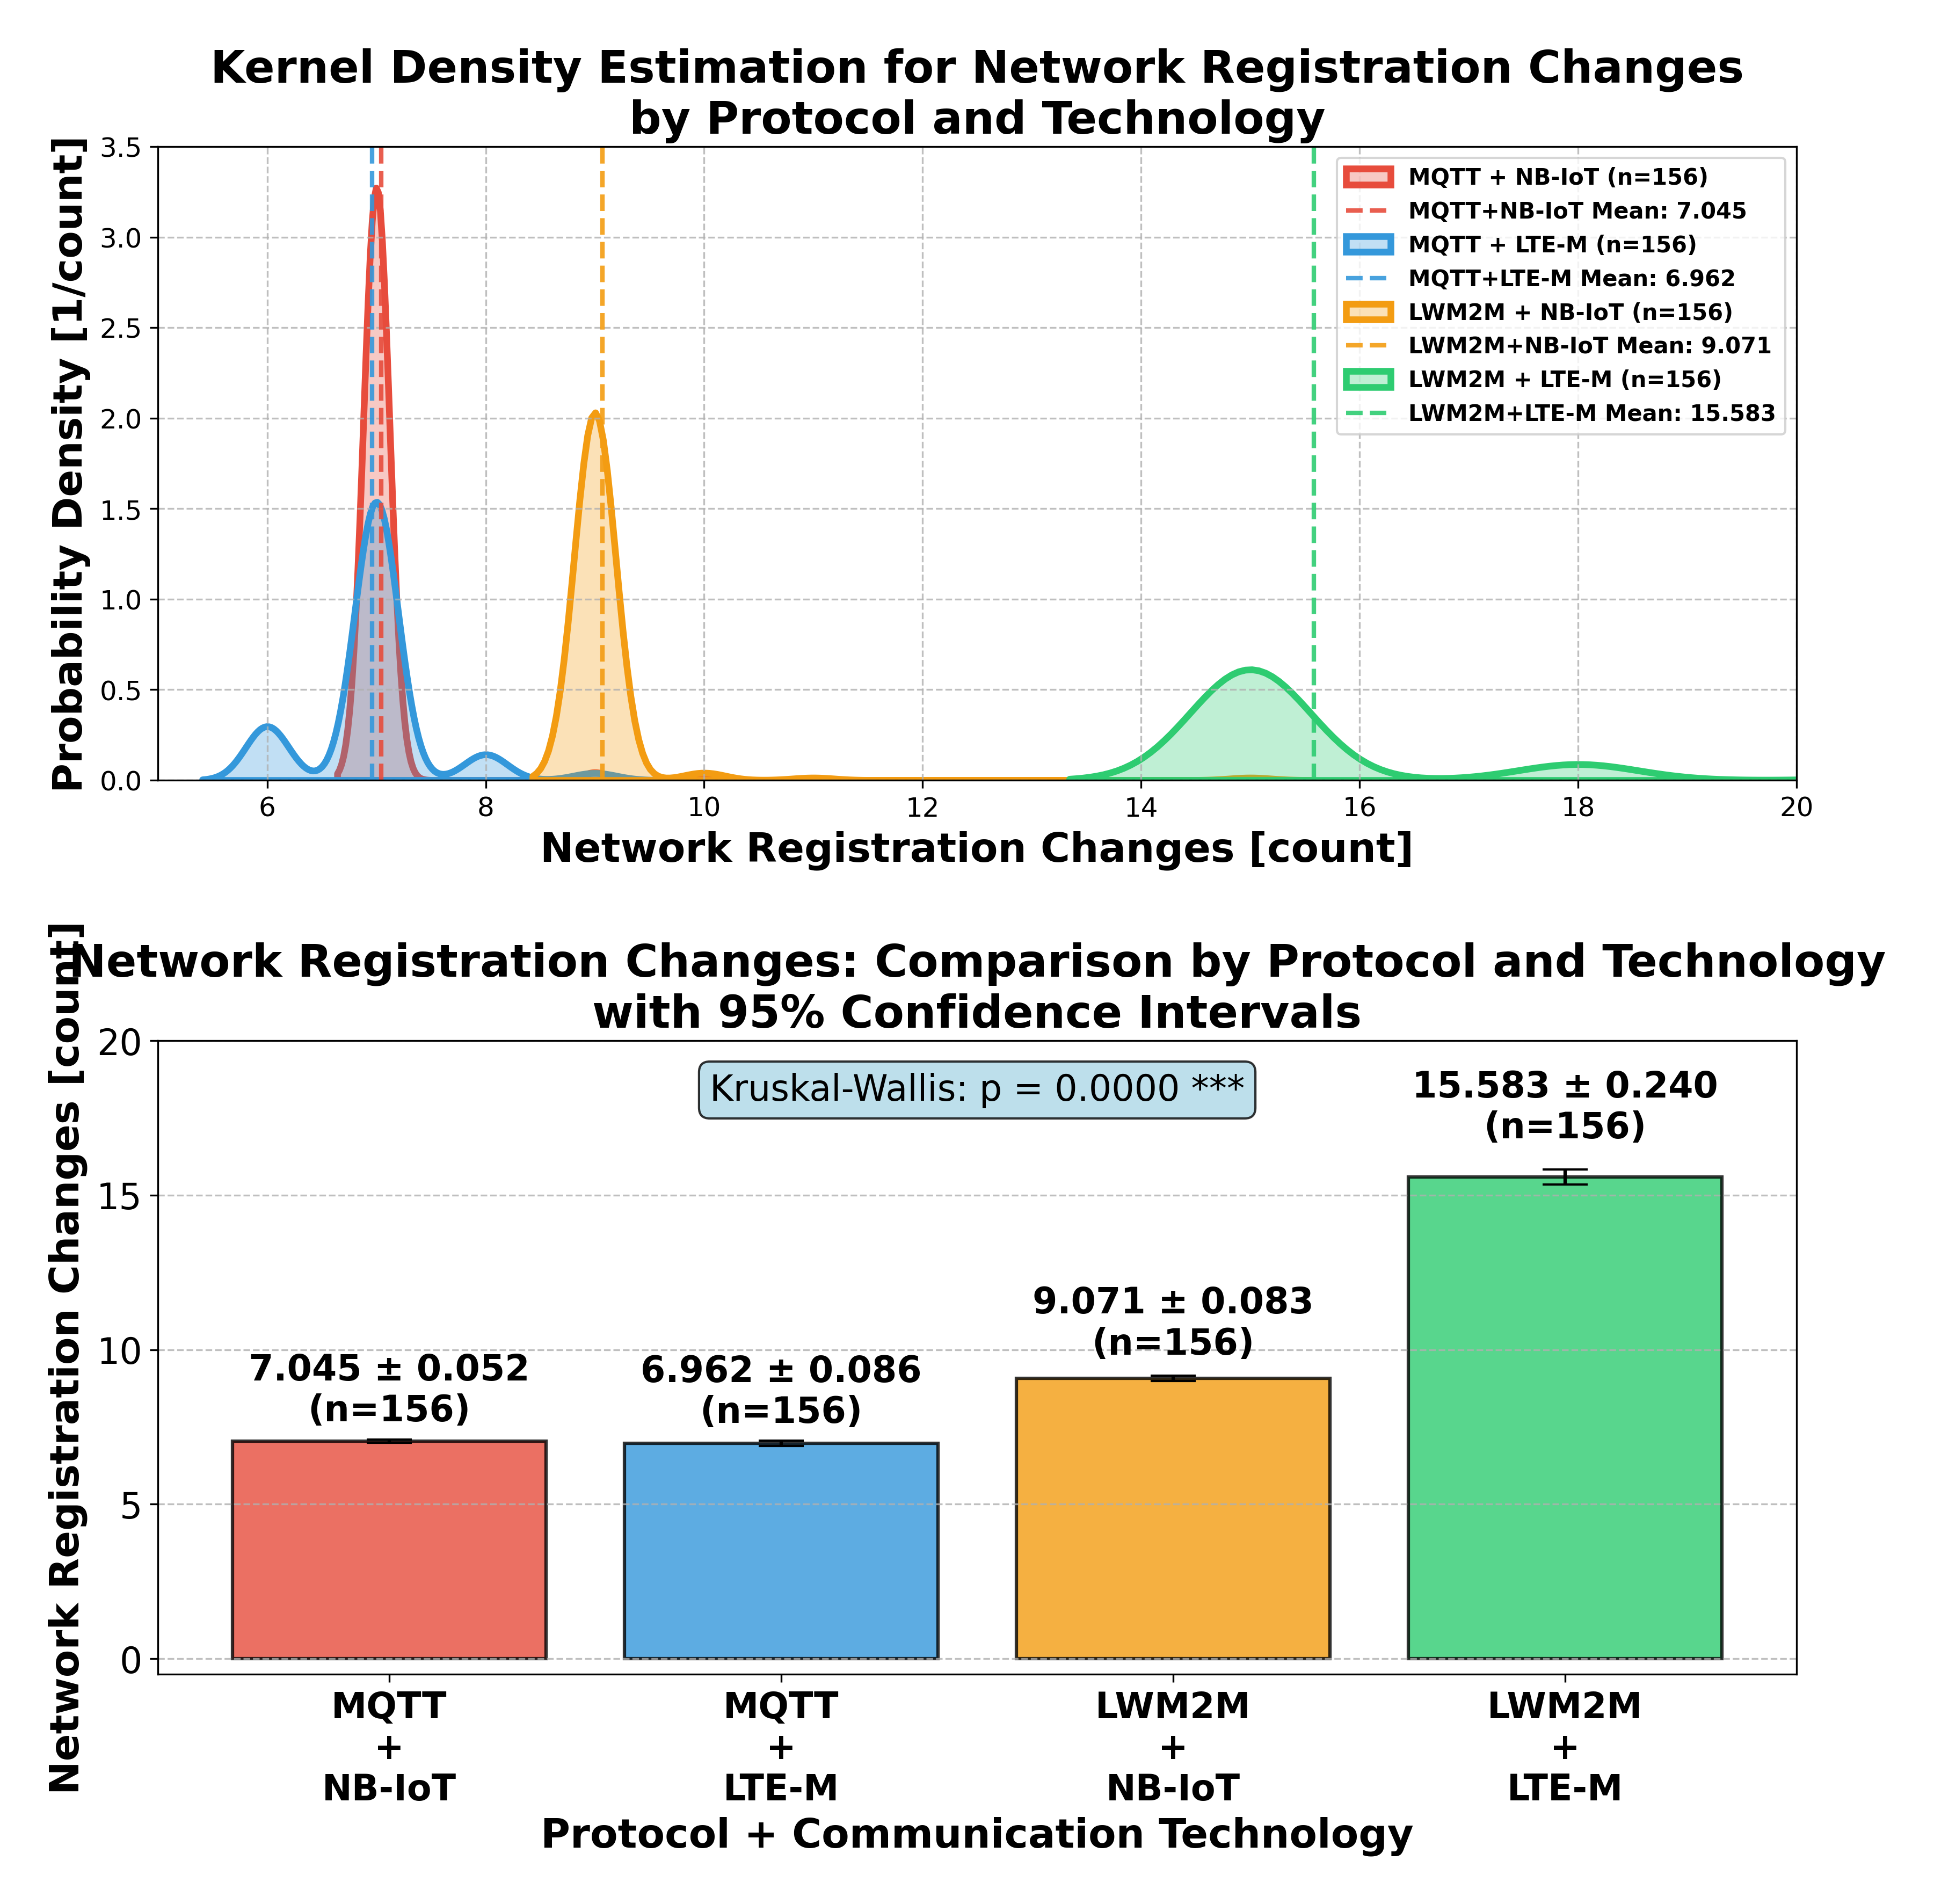
\includegraphics[width=1.0\textwidth]{network_registration_changes_all_protocol_tech_kde_ci.png}
    \caption{\textbf{Network Registration Changes Distribution and Comparison} \\ The figure shows the distribution (top) and confidence interval comparison (bottom) of network registration state changes during communication sessions across different protocol-technology combinations.}
    \label{fig:network_registration_changes_all}
\end{figure}
\FloatBarrier
\subsubsection*{Retransmissions Distribution} \label{sec:retransmissions_analysis}

Figure \ref{fig:retransmissions_all} illustrates the comprehensive retransmission analysis across protocol-technology combinations through integrated distribution and statistical visualization. The KDE analysis demonstrates that \gls{mqtt} over \gls{ltem} achieves the lowest retransmission rate with a mean of 2.109 occurrences, while \gls{lwm2m} over \gls{nbiot} requires the highest number of retransmissions with a mean of 12.833 occurrences. The distribution visualization shows that \gls{lwm2m} over \gls{nbiot} leads to the highest variance in retransmission requirements, whereas \gls{mqtt} over \gls{ltem} shows the most consistent performance with minimal variance. The confidence interval comparison confirms these findings, with the statistical analysis using the Kruskal-Wallis test showing highly significant differences (p < 0.001) in retransmission behavior.

% Figure: Retransmissions Combined
\begin{figure}[htbp]
    \centering
    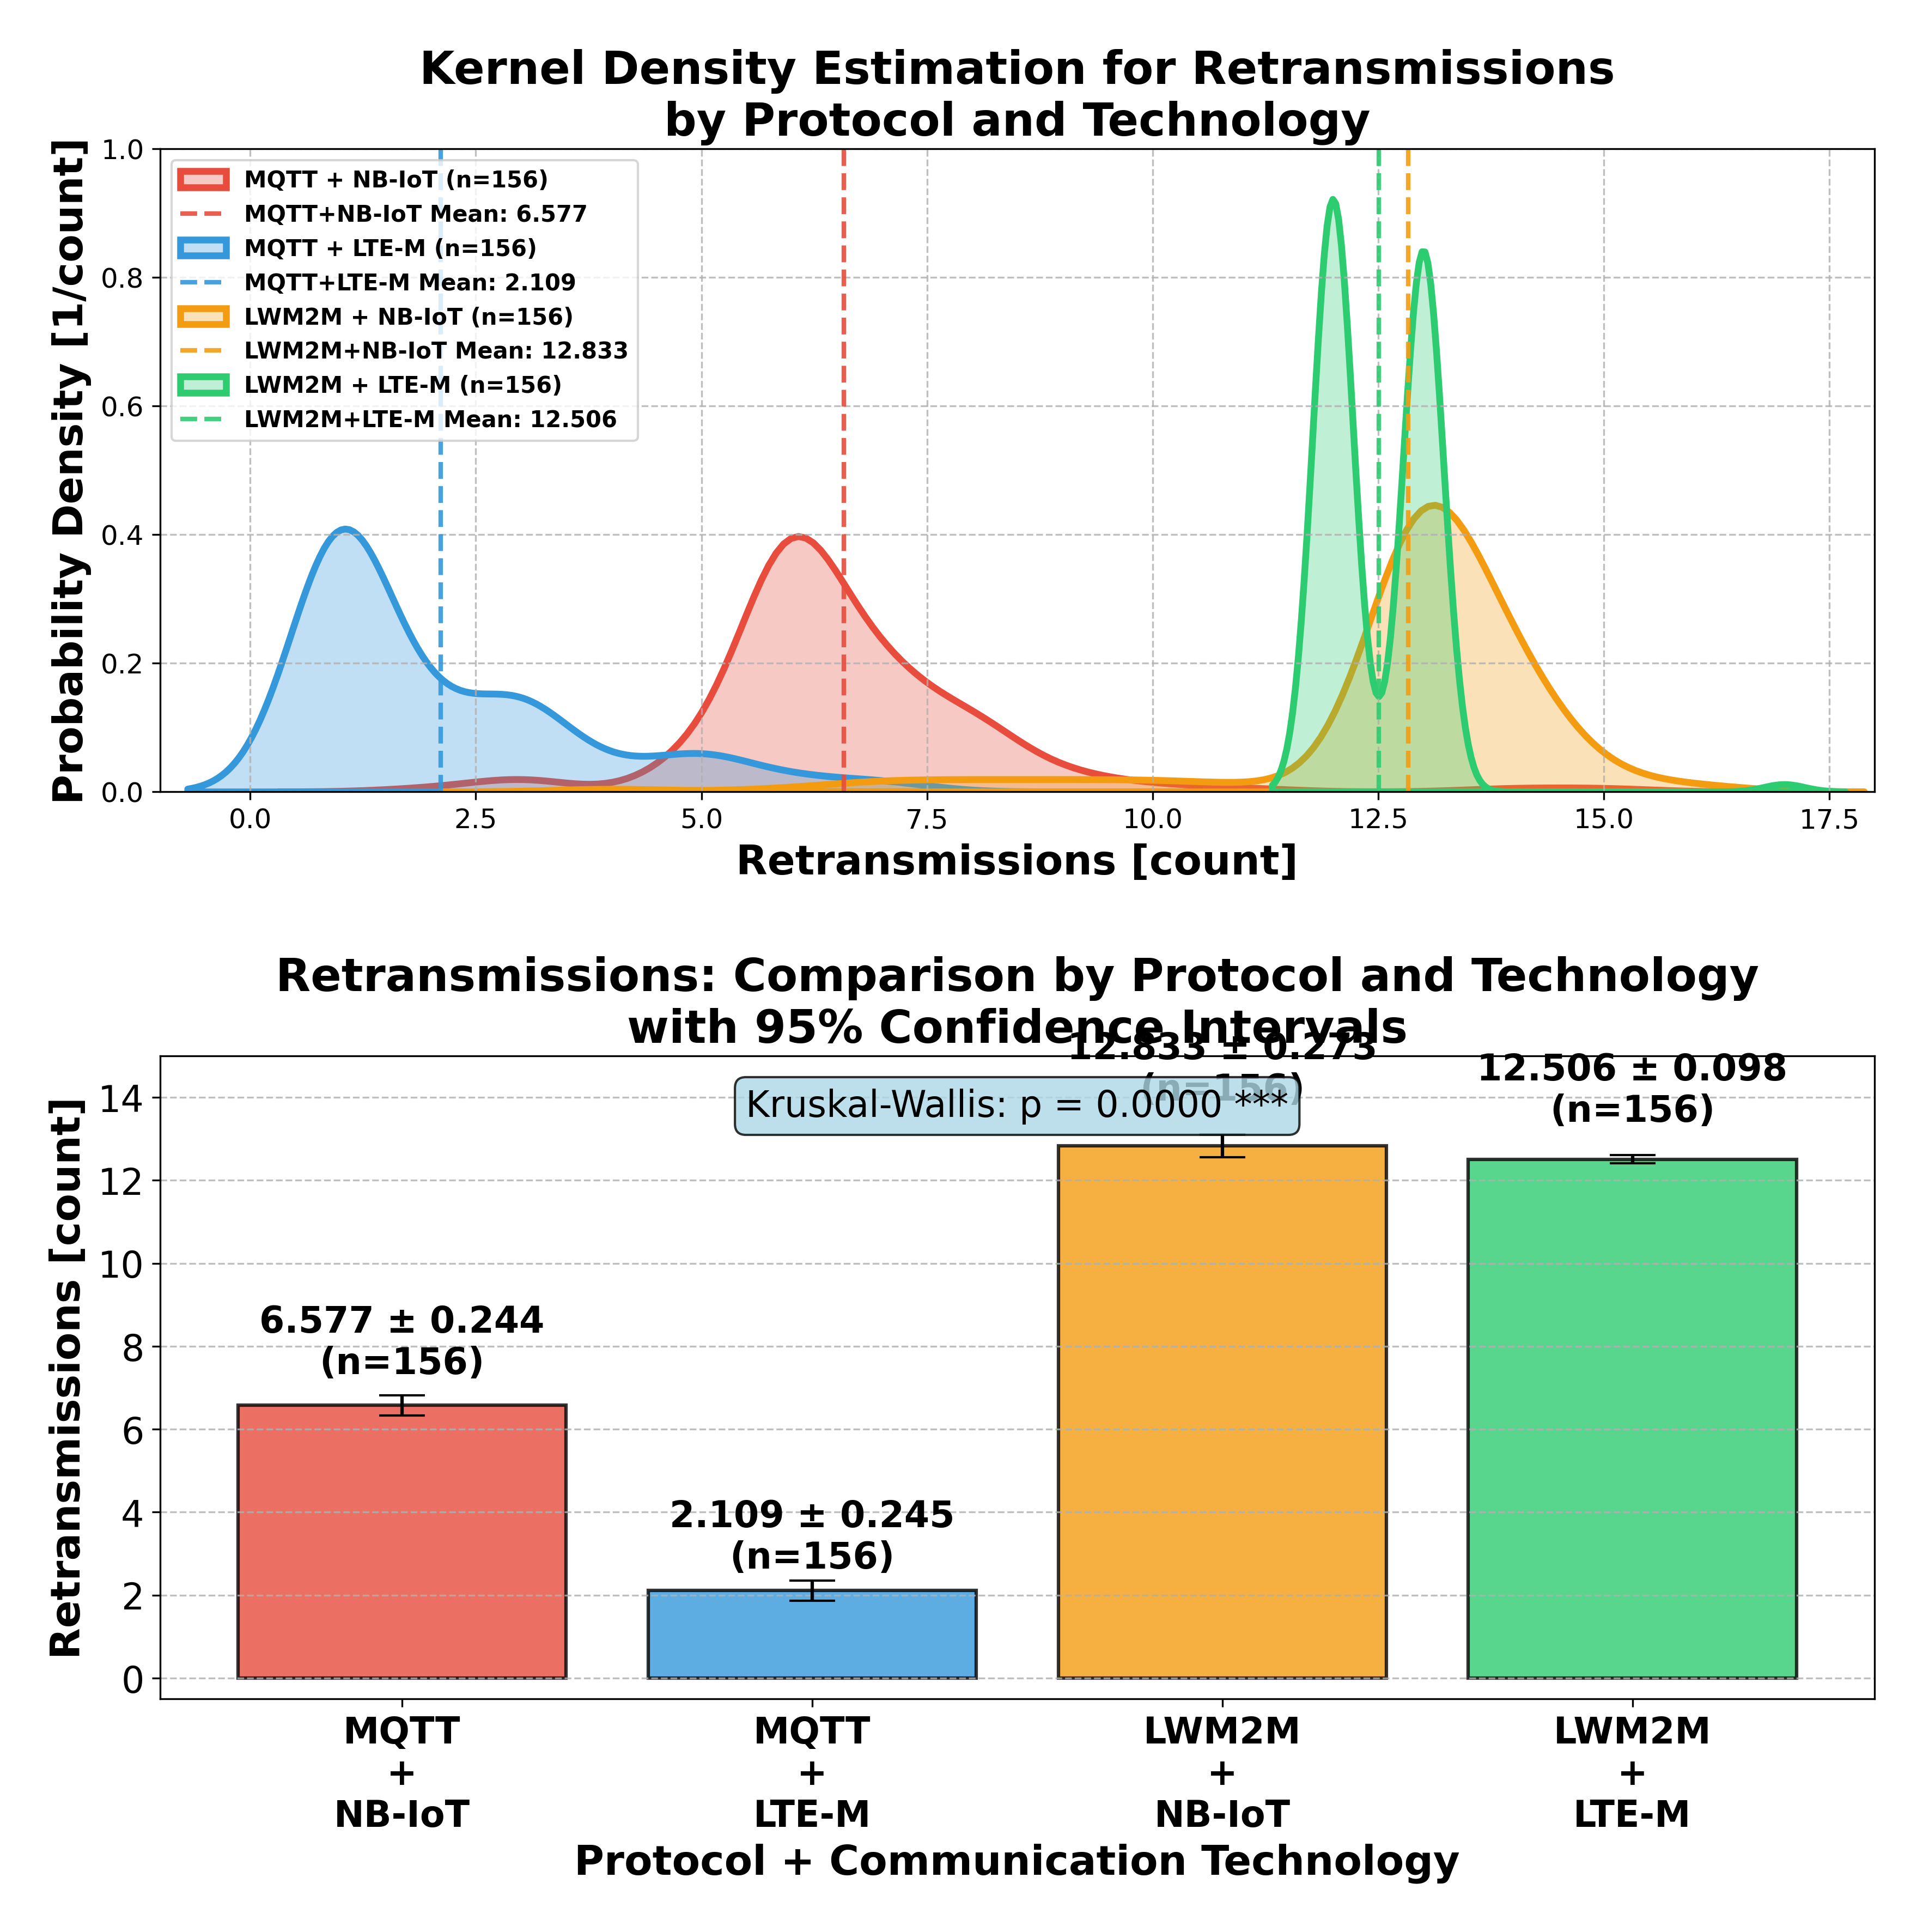
\includegraphics[width=1.0\textwidth]{retransmissions_all_protocol_tech_kde_ci.png}
    \caption{\textbf{Retransmissions Distribution and Comparison} \\ The figure shows the distribution (top) and confidence interval comparison (bottom) of packet retransmissions required during communication sessions, indicating link reliability and protocol efficiency across different combinations.}
    \label{fig:retransmissions_all}
\end{figure}
\FloatBarrier
\subsubsection*{RRC State Changes Analysis} \label{sec:rrc_state_changes_analysis}

The RRC state changes analysis, presented in Figure \ref{fig:rrc_state_changes_all}, provides visualization combining distribution characteristics with statistical comparison. The kernel density estimation shows that \gls{mqtt} over \gls{nbiot} produces the fewest RRC state transitions with a mean of 2.077 occurrences, while \gls{lwm2m} over \gls{ltem} generates the most transitions with a mean of 6.154 occurrences. The distribution analysis reveals that \gls{mqtt} over \gls{nbiot} demonstrates the lowest variance in RRC state changes, indicating stable radio resource utilization, while \gls{lwm2m} over \gls{ltem} exhibits the highest variance in state transition behavior. Statistical testing using the Kruskal-Wallis test, shown in the confidence interval comparison, confirms highly significant differences (p < 0.001) across all combinations.

% Figure: RRC State Changes Combined
\begin{figure}[htbp]
    \centering
    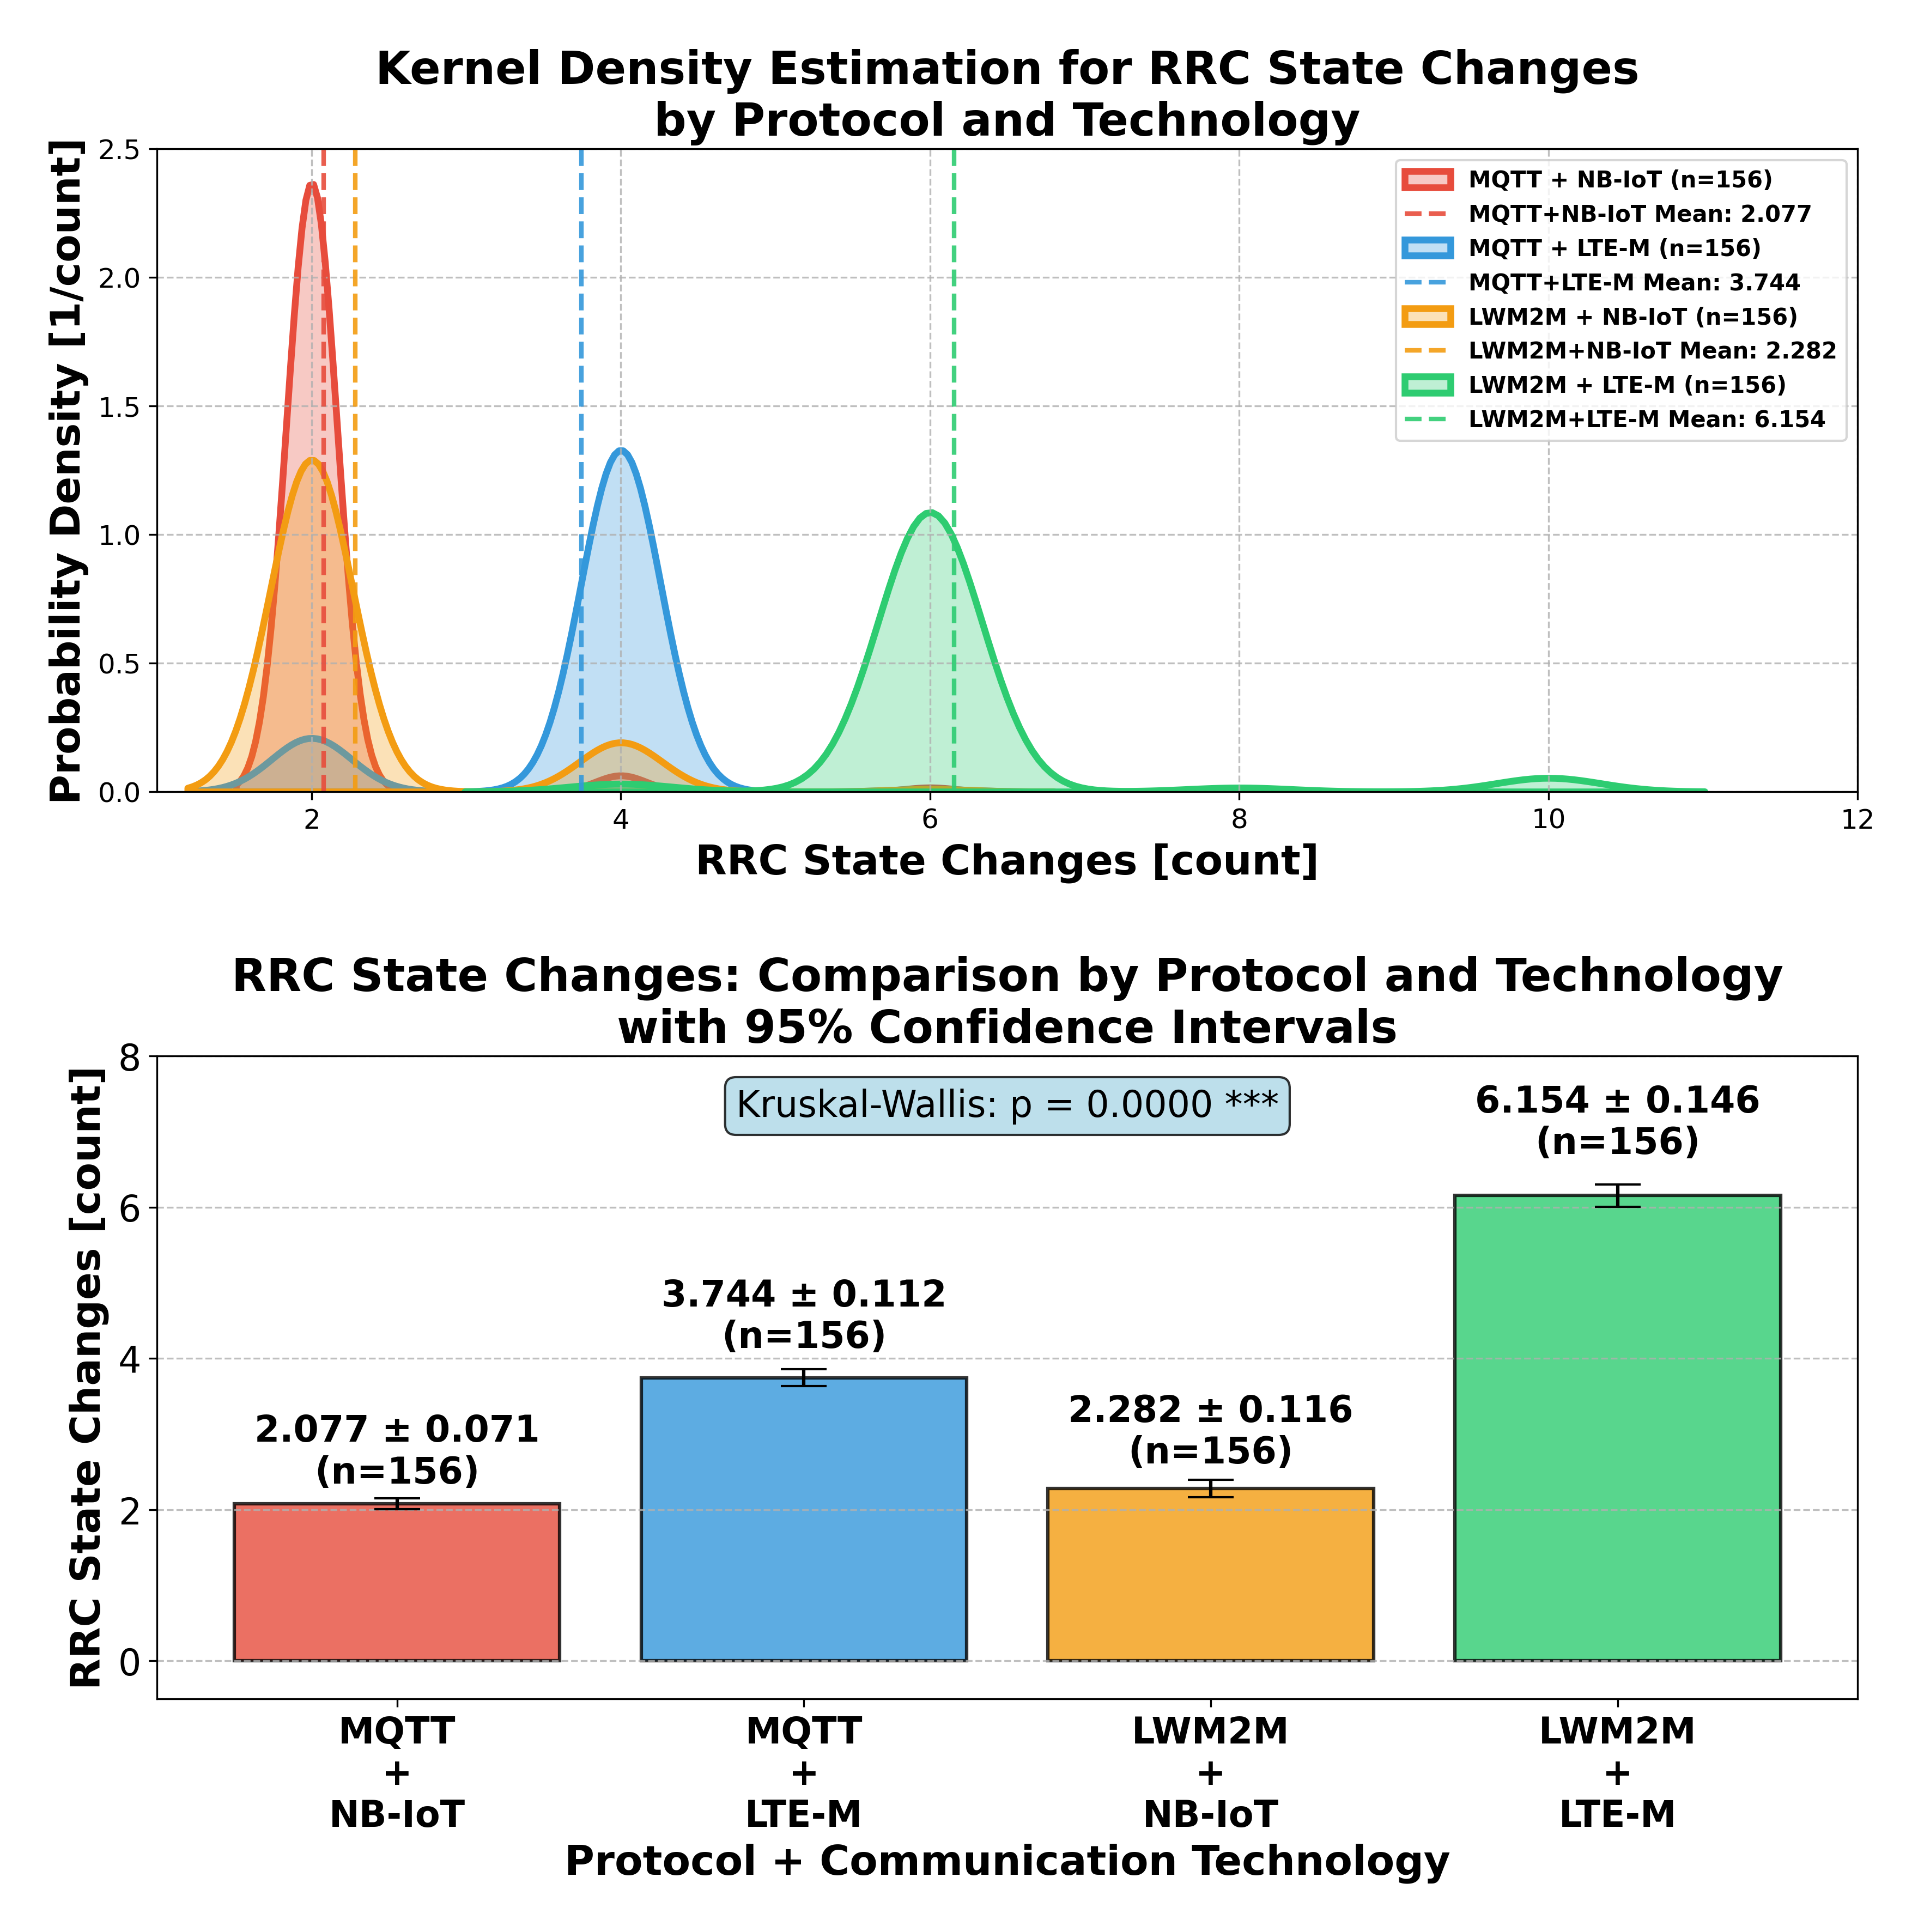
\includegraphics[width=1.0\textwidth]{rrc_state_changes_all_protocol_tech_kde_ci.png}
    \caption{\textbf{RRC State Changes Distribution and Comparison} \\ The figure shows the distribution (top) and confidence interval comparison (bottom) of Radio Resource Control state transitions during communication sessions across different protocol-technology combinations.}
    \label{fig:rrc_state_changes_all}
\end{figure}
\FloatBarrier
\subsubsection*{Protocol and Technology Combination Summary} \label{sec:protocol_technology_combination_summary}

Figure \ref{fig:protocol_technology_combination_summary} provides a full performance summary across all protocol-technology combinations, highlighting the relative strengths and weaknesses of each combination across multiple performance dimensions. The visualization allows identification of optimal combinations for specific application requirements and performance priorities.

% Figure: Protocol and Technology Combination Summary
\begin{figure}[htbp]
    \centering
    \includegraphics[width=1.0\textwidth]{4way_protocol_technology_comparison.png}
    \caption{\textbf{Protocol and Technology Combination Performance Summary} \\ The figure summarizes the performance differences across all protocol and technology combinations. It highlights the strengths and weaknesses of each combination in terms of connection time, latency, retransmissions, and RRC state changes.}
    \label{fig:protocol_technology_combination_summary}
\end{figure}

The protocol and technology combination analysis reveals distinct performance profiles for each configuration. The combined visualization approach, integrating both distribution analysis and statistical comparison, demonstrates that \gls{mqtt} over \gls{ltem} consistently achieves superior performance in latency and connection stability metrics, while \gls{lwm2m} over \gls{nbiot} shows advantages in security handshake efficiency but challenges in overall system responsiveness. These empirical findings provide essential data for informed protocol and technology selection in \gls{iot} deployment scenarios.

\chapter{Discussion} \label{chap:discussion}

This chapter provides an interpretation of the empirical findings presented in Chapter \ref{chap:measurements}, evaluating the performance characteristics of \gls{nbiot} and \gls{ltem} technologies in conjunction with \gls{mqtt} and \gls{lwm2m} protocols for outdoor data collection deployments. The discussion intends to provide the results within the theoretical framework established in Chapter \ref{chap:theoretical_background} and identifies both expected outcomes and surprising findings that came up during the measurements.

\section{Interpretation of results} \label{sec:interpretation_of_results}

The measurement campaign generated a full dataset with 12 radio frequency parameters and 6 protocol-specific metrics across four distinct protocol-technology combinations. The results reveal performance profiles that align with theoretical expectations while also uncovering unexpected behaviors in real-world outdoor deployment scenarios.

\subsection{Signal Quality and Coverage Performance}

The signal quality metrics demonstrate clear differentiation between \gls{nbiot} and \gls{ltem} technologies. As shown in Figure \ref{fig:rsrp}, \gls{nbiot} consistently achieves superior \gls{rsrp} values with a mean approximately 6 dBm higher than \gls{ltem}. This finding aligns with the theoretical coverage enhancement capabilities described in Section \ref{sec:nbiot}, where \gls{nbiot}'s narrowband concentration and repetition coding mechanisms provide up to 20 dB coverage improvement over standard \gls{lte}.

The frequency analysis reveals that both technologies share Band 20 (800 MHz range) while utilizing different additional frequency bands. \gls{nbiot} operates on Band 8 (880-915 MHz uplink, 925-960 MHz downlink) while \gls{ltem} utilizes Band 3 (1710-1785 MHz uplink, 1805-1880 MHz downlink). This frequency allocation pattern contributes to the observed signal quality differences, as the lower frequency bands generally provide better propagation characteristics for outdoor deployments. The shared use of Band 20 by both technologies demonstrates similar performance characteristics in this frequency range, while the additional bands reveal technology-specific optimization strategies.

Similarly, the RSRQ and SNR analyses presented in Figures \ref{fig:rsrq} and \ref{fig:snr} confirm \gls{nbiot}'s signal quality advantages, with mean improvements of 3.5 dB and 3 dB respectively. These results validate the theoretical framework outlined in Section \ref{sec:comparison_nbiot_ltem}, where \gls{nbiot}'s 180 kHz narrowband operation concentrates energy more effectively than \gls{ltem}'s 1.4 MHz bandwidth allocation.

However, an unexpected finding emerged in the variance characteristics of these metrics. While both technologies demonstrate similar RSRP variance, \gls{ltem} shows notably higher RSRQ variance, suggesting more variable signal quality conditions. This contrasts with theoretical expectations that \gls{ltem}'s wider bandwidth would provide more stable signal conditions. The higher variance in \gls{ltem}'s signal quality metrics may be partially attributed to its operation across both lower frequency Band 20 and higher frequency Band 3, which experience different propagation characteristics and interference patterns in outdoor environments.

\subsection{Power Consumption and Energy Efficiency}

The transmit power analysis in Figure \ref{fig:tx_power} reveals that \gls{ltem} requires approximately 3 dBm higher transmit power than \gls{nbiot}, confirming theoretical predictions about \gls{nbiot}'s energy efficiency advantages. This finding is particularly significant for outdoor deployments where sensor nodes must operate on battery power for extended periods in remote locations, as the 3 dBm difference translates to approximately double the power consumption for \gls{ltem} transmissions.

The energy estimate distributions shown in Figure \ref{fig:energy_estimate} present a discrete pattern with three distinct peaks for both technologies. This finding reflects the categorical nature of the energy estimate parameter, which is encoded as discrete integer values by the modem rather than continuous measurements. The observed distribution pattern indicates that both technologies mostly operate within three specific energy consumption classes, likely corresponding to different coverage enhancement levels or network optimization states implemented by the cellular operator.

\subsection{Connection Establishment and Throughput Performance}

The connection time analysis in Figure \ref{fig:connection_time_link} reveals one of the most significant practical differences between the technologies. \gls{nbiot} requires approximately 6.3 seconds more for network attachment compared to \gls{ltem}, which clearly exceeds the theoretical latency specifications outlined in Section \ref{sec:nbiot}. This finding has critical implications for outdoor applications where rapid data transmission may be required during brief weather windows or in response to environmental alerts.

Furthermore, the uplink throughput analysis in Figure \ref{fig:throughput_link} confirms theoretical expectations, with \gls{ltem} achieving approximately 215 kbps higher uplink throughput than \gls{nbiot}. The data shows \gls{nbiot} consistently operating within 0-100 kbps, while \gls{ltem} demonstrates a peak around 300 kbps with a broad uplink distribution spanning 100-380 kbps, aligning closely with theoretical uplink specifications of up to 375 kbps described in Section \ref{sec:ltem}.

\subsection{Limitations of the Study}

While this study provides empirical data on \gls{lpwan} technology and protocol performance for outdoor data collection applications, several limitations must be acknowledged to better understand the findings.

\subsubsection*{Geographic and Environmental Constraints}

The measurement campaign was conducted within a specific geographic region around Cologne, Germany, which may limit the overall generalization of findings to other outdoor deployment environments. Figure \ref{fig:measurement_points_map} shows the spatial distribution of measurement points, which primarily covers urban and suburban environments. The results may not reflect performance characteristics in:

\textbf{Rural and Remote Areas:} Where outdoor experiments and environmental monitoring are commonly executed and cellular coverage characteristics, cell tower density, and interference patterns differ significantly from the measured urban/suburban environment.

\textbf{Different Climatic Conditions:} The measurements were conducted under specific weather and seasonal conditions that may influence radio propagation characteristics relevant to long-term outdoor deployments.

\textbf{International Variations:} Different countries employ varying frequency band allocations, network optimization strategies, and infrastructure deployment patterns that could significantly impact performance metrics for global outdoor monitoring deployments.

\subsubsection*{Measurement Methodology Limitations}

A number of elements of the measurement approach result in limitations on the interpretation of results for applications in outdoor data collection:

\textbf{Single Measurement Per Location:} The study collected only one measurement per geographic location, which may not adequately capture the temporal variability in network performance that outdoor sensors would experience over extended deployment periods. Multiple measurements at each location would have provided better statistical averaging and reduced the impact of temporary network conditions or outlier performance events that could significantly affect long-term outdoor monitoring reliability.

\textbf{Limited Sample Size:} While statistically significant, the overall sample sizes for some parameter combinations may be insufficient to capture important performance events that could significantly impact long-term outdoor deployments. Larger sample sizes with repeated measurements would improve the statistical reliability of the findings and better represent the performance variability experienced in real outdoor monitoring scenarios.

\textbf{Hardware Platform Specificity:} The exclusive use of nRF9160 development kits introduces potential hardware-specific performance characteristics that may not generalize to commercial outdoor monitoring sensor platforms or alternative \gls{iot} device implementations used in environmental research.

\textbf{Protocol Implementation Variations:} The study utilized specific firmware implementations of \gls{mqtt} and \gls{lwm2m} protocols that may not fit to the performance characteristics of optimized commercial implementations used in outdoor monitoring systems.

\textbf{Traffic Pattern Limitations:} The measurement scenarios used fixed payload sizes and transmission patterns that may not accurately represent the diverse data transmission characteristics of real outdoor applications. These characteristics may include variable sensor data sizes, image transmission, or burst data collection patterns.

\chapter{Conclusion} \label{chap:conclusion}

This thesis has conducted a comprehensive performance evaluation of \gls{nbiot} and \gls{ltem} technologies in conjunction with \gls{mqtt} and \gls{lwm2m} protocols for outdoor data collection deployments. Through systematic measurement campaigns and empirical analysis across multiple geographic locations, the study provides evidence-based insights into the practical performance characteristics of these technologies under real-world outdoor conditions.

\section{Summary of Findings}

The empirical investigation reveals distinct performance profiles for each technology-protocol combination, with significant implications for outdoor deployment strategies.

\subsection{Communication Technology Performance}

The comparison between \gls{nbiot} and \gls{ltem} demonstrates clear performance differentiation across multiple dimensions:

\textbf{NB-IoT Advantages:} \gls{nbiot} consistently outperforms \gls{ltem} in signal quality metrics, achieving mean improvements of 6 dBm in \gls{rsrp}, 3.5 dB in \gls{rsrq}, and 3 dB in \gls{snr}. The technology requires approximately 3 dBm lower transmit power, translating to significant energy efficiency advantages for battery-powered outdoor sensors. These findings validate theoretical coverage enhancement claims and confirm \gls{nbiot}'s suitability for challenging outdoor environments where long-term autonomous operation is prioritized.

\textbf{LTE-M Advantages:} \gls{ltem} demonstrates superior performance in connection establishment and uplink data throughput capabilities. The technology achieves network attachment approximately 6.3 seconds faster than \gls{nbiot} and provides 215 kbps higher average uplink throughput, with peak uplink performance reaching 300-380 kbps compared to \gls{nbiot}'s 0-100 kbps range. These characteristics position \gls{ltem} favorably for outdoor applications requiring responsive data transmission or moderate bandwidth requirements.

\textbf{Operational Trade-offs:} The analysis reveals fundamental trade-offs between energy efficiency and performance responsiveness. While \gls{nbiot} offers superior signal quality and energy characteristics, it requires additional transmission repetitions and exhibits higher connection latency. In contrast, \gls{ltem} provides faster, more consistent connectivity at the cost of increased power consumption.

\subsection{Protocol Performance Across Technologies}

The four-way comparison presented in Figure \ref{fig:protocol_technology_combination_summary} reveals that protocol performance is highly dependent on the underlying cellular technology, creating distinct optimization domains for different outdoor deployment scenarios.

\textbf{MQTT Performance Profile:}

\gls{mqtt} demonstrates its most favorable performance when paired with \gls{ltem}, achieving the lowest latency and connection establishment times across all combinations. However, \gls{mqtt} performance degrades significantly on \gls{nbiot}, requiring the longest connection and security handshake times. This degradation suggests that \gls{mqtt}'s \gls{tcp} overhead becomes prohibitive on bandwidth-constrained networks, contradicting theoretical assumptions about protocol scalability.

\textbf{LWM2M Performance Profile:}

\gls{lwm2m} shows unexpectedly poor performance on \gls{nbiot} despite theoretical advantages of UDP-based transport. The combination produces the highest end-to-end latency and retransmission rates, indicating that \gls{coap}'s reliability mechanisms may interact poorly with \gls{nbiot}'s repetition coding mechanisms. This finding challenges theoretical assumptions about \gls{udp} efficiency on constrained networks and suggests that \gls{coap}'s confirmable message semantics may become counterproductive under certain conditions.

\textbf{Session Duration and Protocol Overhead Impact:}

A significant element leading to the surprising performance of the \gls{udp} protocol is the short session duration. The experimental design used very small data payloads and short communication sessions, which reduced the likelihood of connection losses during transmission. Given that \gls{tcp} is sensitive to connection interruptions, where each loss would trigger the overhead of a new handshake, shorter sessions can help minimize the occurrence of this weakness. In such scenarios, the probability of connection loss is reduced, meaning that \gls{tcp}'s handshake overhead is less frequently experienced. Consequently, the potential efficiency advantage of \gls{udp}'s connectionless design becomes less significant in the payload sizes and transmission patterns evaluated in this study.

\subsection{Technology and Protocol Recommendations}

Based on the empirical findings, this study provides evidence-based recommendations for technology selection and deployment strategies in outdoor data collection scenarios.

\textbf{For Long-term Environmental Monitoring:} The deployment of \gls{nbiot} technology for stationary outdoor sensors necessitates an optimal battery life and reliable connectivity, especially in challenging environments. This technology is well-suited for long-term environmental studies, remote agricultural monitoring, and applications with minimal latency requirements.

\textbf{For Responsive Environmental Applications:} Utilize \gls{ltem} for outdoor applications requiring regular connectivity, moderate data rates, or time-sensitive responses. Recommended for real-time environmental alert systems, automated response systems, and research installations requiring frequent data transmission.

\textbf{For Hybrid Deployment Strategies:} Organizations conducting diverse outdoor monitoring activities should consider multi-technology approaches, pushing each technology's strengths for appropriate use cases within the same deployment area.

\textbf{Protocol Selection Recommendations:}

\textbf{MQTT + LTE-M:} Recommended as the primary combination for outdoor applications requiring low-latency sensor data transmission, integration with established \gls{iot} ecosystems, and moderate data rates. The combination provides the most predictable and efficient performance profile for responsive environmental monitoring systems.

\textbf{LWM2M + LTE-M:} Suitable for outdoor monitoring systems requiring remote device management capabilities, firmware updates, and complex configuration management.

\textbf{MQTT + NB-IoT:} Use only for applications with minimal latency requirements and infrequent communication patterns, such as daily environmental logging.

\textbf{LWM2M + NB-IoT:} Generally not recommended due to poor latency performance and high retransmission rates, except for specialized device management scenarios where security handshake efficiency is prioritized.

\subsection{Research Contributions}

This thesis makes several significant contributions to the understanding of \gls{lpwan} technology performance for outdoor data collection applications:

\textbf{Empirical Evaluation:} The study provides empirical evaluation that simultaneously examines both communication technology performance (\gls{nbiot} vs. \gls{ltem}) and protocol behavior (\gls{mqtt} vs. \gls{lwm2m}) under identical outdoor conditions, addressing a critical gap in existing literature.

\textbf{Protocol-Technology Interaction Analysis:} The identification and quantification of protocol-technology interaction dependencies provides new insights that challenge conventional assumptions about protocol efficiency on constrained networks, particularly the unexpected poor performance of \gls{udp}-based protocols on bandwidth-constrained networks.

\textbf{Real-World Performance Validation:} The empirical validation of theoretical specifications has revealed significant differences between standardized performance specifications and practical deployment reality, providing valuable data for future standardization efforts and deployment planning.

\textbf{Statistical Performance Characterization:} The statistical analysis using Mann-Whitney U and Kruskal-Wallis tests provides robust validation of the observed performance differences, ensuring confidence in the practical significance of the findings.

\textbf{Methodological Framework:} The development of a reproducible measurement framework and automated data collection system provides a foundation for future research in outdoor \gls{lpwan} performance evaluation.

\chapter{Outlook} \label{chap:outlook}

This chapter presents an overview of future advancements and potential enhancements in the area of outdoor data collection using \gls{lpwan} technologies.

While this study provides a detailed performance characterization of \gls{nbiot} and \gls{ltem} in combination with \gls{mqtt} and \gls{lwm2m} for outdoor data collection, several extensions could enhance the applicability and generality of the findings. Future research should include repeated measurements at each location to capture temporal variability and enhance statistical reliability. The geographic scope should be expanded to include rural and remote areas, and multi-operator evaluations should be performed to provide broader coverage of real-world deployment conditions. The use of diverse hardware platforms and the implementation of optimized commercial protocols could potentially reveal hardware- and software-specific effects that were not captured in this study. Furthermore, integrating variable payload sizes and more authentic traffic patterns would facilitate performance evaluation under a broader spectrum of operational scenarios relevant to outdoor monitoring applications.

A notable observation in this study was that the short session duration and very small payload sizes reduced the likelihood of connection losses during transmission. Given the sensitivity of \gls{tcp} to connection interruptions, where each loss triggers the overhead of a new handshake, shorter sessions have been shown to minimize the occurrence of this weakness. Therefore, \gls{tcp}'s handshake overhead was barely experienced, and the potential efficiency advantage of \gls{udp}'s connectionless design became less significant under the tested conditions. To further investigate this effect, future experiments should include longer connection sessions and varied payload sizes to evaluate whether differences in \gls{udp} and \gls{tcp} performance become more apparent when connection losses are more likely to occur. Such investigations would help clarify protocol behavior in deployment scenarios involving continued data flows or more challenging network conditions.

\clearpage
\section*{Tools Used}
\addcontentsline{toc}{section}{Tools Used}
In the course of creating this work, the following tools and resources were used to assist:

\begin{itemize}
    \item ChatGPT (OpenAI)
    \item Claude Sonnet (Anthropic)
    \item DeepL Translator
    \item MacTex
    \item VS Code (Visual Studio Code)
    \item GitHub Copilot
\end{itemize}

\chapter{Acknowledgements} \label{chap:acknowledgements}
I would like to thank everyone who supported and encouraged me during the preparation of this master’s thesis.

First, I am grateful to Professor Dr. Uwe Dettmar for supervising my work and for his valuable guidance in developing ideas over the past years. I would also like to thank my colleagues and fellow students at the Institute of Digital Communication for their constructive discussions and practical advice.

Special thanks go to Dipl.-Ing. Martin Seckler for his patient and reliable help with numerous measurements and technical challenges, and to Professor Dr. Harald Elders-Boll for serving as co-examiner.

Finally, I am deeply thankful to my parents, my brother, and my friends for their support throughout my studies.

\chapter*{Erklärung}
%
Ich versichere, die von mir vorgelegte Arbeit selbstständig verfasst zu haben. Alle Stellen, die wörtlich oder sinngemäß aus veröffentlichten oder nicht veröffentlichten Arbeiten anderer oder der Verfasserin/des Verfassers selbst entnommen sind, habe ich als entnommen kenntlich gemacht. Sämtliche Quellen und Hilfsmittel, die ich für die Arbeit benutzt habe, sind angegeben. Die Arbeit hat mit gleichem Inhalt bzw.\ in wesentlichen Teilen noch keiner anderen Prüfungsbehörde vorgelegen.
\par
\\[3cm]
%
\begin{tabular}{@{}l@{}}%
    \rule{0.35\textwidth}{0.4pt} \\
    Ort, Datum%
\end{tabular}%
\hfill%
\begin{tabular}{@{}l@{}}%
    \rule{0.45\textwidth}{0.4pt} \\
    Unterschrift%
\end{tabular}%

\listoffigures
\listoftables
\printglossary[type=acronym]
\printbibliography

\end{document}
